\documentclass[12pt]{article}

\usepackage{graphicx} % Support for including graphics
\usepackage{mathptmx} % Set font to Times New Roman
\usepackage{geometry} % Margins
\usepackage{multirow} % Tables
\usepackage{float}
\usepackage{amsmath}
\usepackage{listings}
\usepackage{xcolor}
\usepackage[affil-it]{authblk}
\usepackage{hyperref}

\definecolor{backcolour}{rgb}{0.95,0.95,0.92}

\lstdefinestyle{yaml}{
  basicstyle=\color{blue}\footnotesize,
  backgroundcolor=\color{backcolour},   
  rulecolor=\color{black},
  string=[s]{'}{'},
  stringstyle=\color{blue},
  comment=[l]{:},
  commentstyle=\color{black},
  numbers=left,                    
  morecomment=[l]{-}
}

\lstset{style=yaml}

\geometry{
  a4paper,
  left=35mm,
  right=30mm,
  top=30mm,
  bottom=30mm
}

\title{Efficient vision-based hand gesture recognition on low-power devices}
\author{Rodrigue Denis GASPARD}
\affil{Master of Computer Science \\ UniKL \\ MIIT Campus}
\date{\today}

\clearpage

\begin{document}

\maketitle

\clearpage

\tableofcontents

\clearpage

\begin{table}
  \centering
  \begin{tabular}{ |p{3cm}|p{8cm}|  }
    \hline
    \multicolumn{2}{|c|}{Abbreviations used in this thesis} \\
    \hline
    Acronym & Meaning \\
    \hline
    ASL & A visual language used by the deaf community in the U.S. and Canada.\\
    HGR & Technology that interprets human hand movements as commands. \\  
    CNN & A type of deep learning model primarily used for analyzing visual data. \\
    CPU & The main processor that executes instructions in a computer. \\
    GPU & A specialized processor designed to accelerate graphics rendering. \\
    EMG & A technique for recording electrical activity produced by skeletal muscles. \\
    SBC & A complete computer built on a single circuit board. \\
    IoT & A network of interconnected devices that communicate over the internet. \\
    ToF & Technology that measures distance by calculating the time light takes to travel to an object. \\
    ISA & Defines the set of instructions a processor can execute. \\
    IR  & Electromagnetic radiation with wavelengths longer than visible light. \\
    FPS & The number of frames displayed or processed in one second. \\
    CFS & A method for selecting relevant features in a dataset based on correlation. \\
    Ghz & A measurement of frequency equal to one billion hertz. \\
    SGD & An optimization algorithm used to update weights in machine learning models. \\
    TDP & The maximum amount of heat generated by a computer chip under load. \\
    mAP & A metric used to evaluate the accuracy of object detection models. \\
    \hline
  \end{tabular}
\end{table}

\clearpage

\begin{abstract}
The democratization of edge devices is transforming the landscape of human-computer interaction, necessitating innovative interface modalities. Among these, vision-based recognition stands out as a highly suitable approach to facilitate this shift. With the advent of affordable and user-friendly single-board computers that possess adequate processing power, real-time hand gesture recognition is becoming increasingly feasible. This thesis explores the application of advanced deep learning techniques, specifically the You Only Look Once (YOLO) model, which has demonstrated remarkable performance, achieving over 99\% in mean Average Precision at 50\% Intersection over Union (mAP50).

While pose estimation offers a nuanced understanding of human gestures providing valuable depth compared to simple object detection, it is inherently more computationally intensive. Despite its increased complexity, pose estimation can achieve comparable inference times as object detection, a critical factor in real-time application scenarios. 

Our tests reveal that a mid-range Dell laptop yields an inference time of approximately 50 milliseconds for both object detection and pose estimation, making it suitable for practical applications in real-time gesture recognition. In contrast, experiments conducted on a Raspberry Pi indicate an inference time exceeding 300 milliseconds, presenting significant challenges for deployment in real-time systems.

This thesis ultimately underscores the potential of leveraging vision-based recognition in edge devices while identifying key performance metrics and hardware constraints that must be addressed to fully realize the promise of real-time human-computer interaction in diverse applications. Through this exploration, we aim to contribute to the ongoing dialogue regarding the enhancement of user interfaces in a ever-changing technological landscape.
\end{abstract}

\clearpage

\section{Introduction}

\subsection{Background}

To interface with machines, humans have used a plethora of peripherals of techniques in the past. The keyboard, which is straightforward and was already familiar to users as it used for typewriters and pointer devices such as the computer mouse. Then came remote controllers, either by radio or infrared signals, or by Bluetooth/Wi-Fi technology, which allows more freedom of movement to the user, instead of being constrained to the close locality of the machine being used.

However, those methods often required some kind of training from the user in order to be able to use the machine. The idea of controlling devices remotely using body language or voice commands, which offers both flexibility and user-friendliness compared to the previously mentioned techniques, became a viable option around the end of the century.

Voice-assisted technology allows users to interact with devices and software through spoken commands. It usually involves speech recognition, which converts spoken words into text or commands, by detecting and tokenizing phonemes, words, and sentences. Text-to-speech, also known as TTS, converts text input into spoken language with the help of synthesizers to produce speech, sometimes conveying emotions with impressive results, as demonstrated by OpenAI's ChatGPT-4o. A notable example for voice recognition was Dragon NaturallySpeaking, a proprietary software recognition package released by Dragon Systems in 1996, which was one of the first voice assistants available to the public, and allowed for continuous recognition.

Hand and body gesture recognition refers to the analysis of movements made by the hands, arms, and body to understand the intended actions or expressions. It can involve only specific parts of the body, for example the face, to detect sentiments, for facial recognition by focusing on key features and cross-reference them in a database in order to get the individual's identity. It can also be used to capture input and mimic them in a skeleton-based approach to a 3d model for animation/special effects purposes.
Gesture recognition can also involve the whole body, usually for motion capture, gait analysis, or for various security reasons (concealed weapon and theft detection).

The focus of this paper is hand gesture recognition, as it provides several advantages compared to full-body or facial motion capture. First, hand gestures can convey a lot of information easily, as demonstrated by the several visual languages, also called sign languages. The most full-fledged sign language is often considered to be American Sign Language (ASL). ASL is a complete, complex language with its own grammar, syntax, and vocabulary, distinct from English. It is widely used within the deaf community in the United States and parts of Canada.
ASL also integrates fingerspelling, where each letter of the Latin alphabet is represented by a distinct hand gesture or sign. It is typically used to spell out proper nouns, technical terms, or words that do not have an established sign in a particular sign language. Fingerspelling allows users to communicate words or concepts that may be difficult to represent with standard signs, such as names, addresses, or specialized vocabulary. Thus, one can convey rich and complex ideas using only their hands, without requiring additional context or verbal and non-verbal cues.

Hand gesture recognition is also more flexible and natural than full-body or facial recognition, it does not require as much space as full-body recognition and can be used more easily and naturally than facial recognition (it does not require looking straight at the camera with a specific intent). It also allows for people with mobility issues to use this system with ease, without straining their body or exerting too much energy.
Furthermore, hand gestures can take many forms (fist clenched, palm opened, any number of fingers extended or retracted), thus are very clearly identifiable between one another. This can help to lower the computational complexity required to detect the gestures and increase the mean accuracy of the detections, making the technology more reliable when applied as a human-machine interface. Finally, multi-user interfacing, that is detect several hand signals at the same time from multiple agents is easier to implement, as the requirements for efficient detection are low compared to full-body or facial detection. 

\subsubsection{Static and dynamic hand gestures}

Hand gestures can be classified in two categories : static and dynamic.
In static hand gesture recognition, the system identifies gestures that involve a single posture or shape of the hand that remains relatively fixed in space. It focuses on recognizing hand configurations or positions without considering movement over time. For example, recognizing a hand gesture showing a specific number of fingers (a thumbs-up, the "peace" sign, or the number four). These gestures can be simply detected using techniques such as shape analysis or contour detection from single frames, as there is no notion of time tied to the meaning of the hand gesture.

Thus, it's often considered simpler to implement than dynamic recognition, as it only requires capturing a single frame or static pose. It's also well-suited for tasks where the hand gesture is briefly held (recognizing numbers or simple commands, such as manipulating basic software). However, for more complex applications (sign language interpreter, complex software interactions such as drawing or gaming), this approach might not be enough to convey the actions of the user in detail.

Dynamic hand gesture recognition involves detecting and interpreting gestures that include hand movement over time. This type of recognition analyzes not only the shape and position of the hand but also the trajectory, speed, and changes in hand posture across a sequence of frames. Waving "goodbye", pointing in a specific direction, pinching, or drawing shapes using your hands are all examples of dynamic hand gestures. Dynamic gestures require tracking the hand over multiple frames to capture motion, often using optical flow or skeletal tracking, the former being the apparent motion of objects in a visual scene caused by the relative movement between the camera (or observer) and the objects, and the latter being a computer vision technique used to detect and track the position of a human body or hand by identifying key points (or joints) that make up the "skeleton" of a person or limb.

While dynamic hand gesture recognition can capture more complex and rich gestures, and can also be more suitable for real-time applications, such as controlling devices through continuous hand gestures (navigating a menu by swiping or controlling a robot or a drone), it is more computationally intensive than static hand gesture recognition because it requires processing and analyzing multiple frames, which can be challenging for real-time applications, and it can be sensitive to speed variations in the gesture execution, requiring robust algorithms and fine-tuning to account for temporal differences.

We will focus on static hand gesture recognition for this thesis. As we're focusing on low-power devices with limited computational power, static hand gesture recognition is more suited for these conditions, and it can still provide enough information for basic applications, such as manipulating a video player.

\subsubsection{Detection techniques}

In order to capture the movements of the human body and translate it into input for a computer, special hardware is often required. We can classify those sensors into two broad categories : sensor-based and vision-based \cite{qi2024computer}.
The sensor-based approach uses a variety of different techniques, namely :
\begin{itemize}
  \item Glove-based approach, which uses gloves with a wide range of sensors, that the user must wear in order to input finger or hand movement for detection. These sensors include, but are not limited to flex sensors, which records the bending and movement of individual fingers, accelerometers and gyroscopes which track the movement and rotation of the hand and pressure/force sensors, which can be used to detect clenching or pinching. While they are considered the most reliable way to detect hand gestures due to the rich and precise data they provide, they're not always suited for most applications as you need to wear the gloves at all times in order to detect hand gestures. They're also not the most cost-effective way of making detections, as the gloves requires special, often expensive sensors and specific tailoring for the user.
  \item Electromyography, or EMG, can also be used for detection, by measuring the electrical activity produced by skeletal muscles when they contract. By placing electrodes on the surface of the skin at specific points, it is possible to capture the electrical signals generated by muscle activity in the hand and forearm. These signals vary depending on the type of movement or gesture being performed. Much like the data gloves, it can achieve extreme levels of accuracy, but suffers from the same problems, the equipment required is not readily available and can be expensive, and the user has to have the electrodes at all times during the detection process. Furthermore, EMG signals can wildly vary between individuals depending upon several factors (age, physical fitness, medical conditions, medications, etc.) resulting in noise and false readings. Finally, correct electrode placement can be tedious without prior medical anatomical and medical knowledge.
  \item Detecting using radio or Wi-Fi waves, which leverages the way wireless signals interact with human movement. Both technologies exploit changes in the reflection, absorption, scattering or frequency (Doppler shift \cite{kim2016hand}) of wireless signals caused by hand movements to recognize gestures. While these techniques might not always require wearable sensors, can be readily available and cost-efficient in the case of Wi-Fi detection, and have decent range and accuracy, they are still subjected to perturbations like signal congestion, variations of signal strength, and in the case of radar detection, can be power-hungry and a concern for low-power devices.
\end{itemize}

The vision-based approach refers to using computer vision techniques to detect, track, and recognize hand movements or postures from visual data, typically captured by cameras or optical sensors. This approach relies on image or video processing algorithms to interpret gestures in real-time or from recorded footage. The entire process revolves around using almost exclusively visual data rather than external sensors like gloves or electrodes, which makes it non-intrusive and more convenient for real-world applications. However, challenges such as lighting conditions, background complexity, and occlusions can impact the accuracy of this method. It is generally considered less accurate overall than the sensor-based approach.

For this paper, I chose to explore the vision-based approach over the sensor-based one for detection for several reasons :

\begin{itemize}
  \item The vision-based approach is easier to implement than other methods, as it only relies on visual data, typically in the visible or infrared spectrum. There are several techniques available for detection and there are a lot of datasets in relation to hand gesture recognition available, making the machine learning and deep learning detection approach simple to implement. 
  \item Vision-based systems capture gestures from a distance without the need for wearable devices like gloves or sensors. This makes the interaction more natural and intuitive for users. Also, in relation to low-power and embedded devices which often need to be as compact and portable as possible, this approach is more suited as it only requires a camera.
  \item Multiple users can perform gestures at the same time, and vision-based systems can handle these inputs concurrently without interference, which is more difficult with sensor-based approaches.
  \item Vision-based systems can scale to large spaces and public installations, such as in smart homes, interactive displays, or public settings, where sensor-based systems might be impractical due to range and hardware limitations.
  \item Vision-based techniques approximate how humans perceive gestures, making it easier to design systems that feel intuitive and human-centered. The raw data input is also more intuitive than the sensor-based techniques, where prior knowledge in physics (radar or Wi-Fi detection makes use of wave theory, and EMG requires basic understanding on how muscles works)
\end{itemize}

The focus of this paper being low-power devices, where power efficiency being crucial, it is important to talk about the hardware constraints. Most low-power devices do not come with the processing power necessary for complex tasks, such as training deep learning models. Most SBCs only comes with a central processing unit and no graphical processing unit, due to the power restrictions.
The central processing unit, also called CPU, is the primary component of a computer responsible for carrying out general-purpose tasks, including arithmetic, logic, control, and input/output operations. It is designed to handle a wide range of tasks sequentially, making it a versatile processor for a variety of computing needs. Modern CPUs have multiple cores, allowing them to handle some parallelism, but they are still optimized for serial tasks.

The graphical processing unit, or GPU, on the other hand is specialized hardware originally designed to accelerate the rendering of images and videos, especially for gaming and other graphical tasks. Unlike CPUs, GPUs have a large number of smaller, more efficient cores designed to handle many parallel tasks simultaneously. This architecture makes them highly effective for tasks that require processing large amounts of data in parallel, such as matrix and vector operations. Unlike CPUs, GPUs typically have hundreds to thounsand smaller cores, each with different functions. The NVIDIA RTX 4090 has more than 16,384 CUDA cores, design to accelerate parallel processing tasks. It's generally considered essential for training deep learning models, large datasets, and high-dimensional computations and can dramatically speed up the training time for deep learning models, usually by one of two orders of magnitude.

CPUs comes in different core architectures, which is the underlying design and structure of a CPU's processing core, which is responsible for executing instructions and performing computations in a computer. Different core architecture have different instruction set architectures (ISAs) and optimizations and special support for AI-specific instructions. The ISA defines the set of instructions the CPU can execute, such as arithmetic operations (add, subtract, etc.), memory operations (load, store), and control operations (branching). Common ISAs include x86, used by Intel and AMD processors, and ARM, used in mobile devices and some SBCs such as the Raspberry Pi.
Intel processors usually have better single-core performance than AMD processors, but they also have special features such as DL Boost. Deep Learning Boost (DL Boost) introduced in recent Intel processors is designed to accelerate AI workloads, especially inference, by optimizing low-precision calculations (INT8). This feature is useful in speeding up inferencing for ML models like neural networks.
On the other hand, AMD usually offer more cores and threads at a lower price point than Intel, and are often the choice for embedded or mobile devices. More cores can be helpful when training ML models, especially for large datasets and parallelized workloads. AMD does not have a direct analog to Intel's DL Boost, however.

\subsection{Problem statement}

With the democratization of handheld devices, smart home appliances,  virtual and augmented reality environments, and the emphasis on accessibility in software development, new ways to interact with technology are required in order to bridge the gap between man and machine, and to capitalize on the portable access of these devices. 

Several methods and technologies aims to tackle this issue, such as voice-assist, motion capture, gesture recognition, eye-tracking technology, and so on. 

However, compared to traditional computer peripherals, those often requires specific hardware requirements, extensive data as well as complex and resource-intensive algorithms. For facial or hand-gesture recognition, a graphical processing unit is often necessary for real-time applications. Unfortunately, this increase manufacturing costs significantly, and requires more power, the latter being a heavy constraint for embedded devices, single-board computers and other low-power devices.
Thus, optimizing existing algorithms for CPU-only environments might allow those devices to perform more tasks and make them more accessible. Most research done on those algorithms use powerful GPUs in order to drastically increase performance and reduce training time, sometimes by several orders of magnitude. As a result, this creates a research gap when it comes of benchmarking deep-learning models on CPU-only environments.

In addition, detecting and processing hand gestures in real-time, as in interpreting the contents over a live video feed and outputting a prediction in a reasonable short interval in order to interact in a fluid manner with a computer, presents several challenges to overcome.
In real-time systems, gestures must be processed almost instantaneously to ensure a seamless user experience. Any delay between the gesture being made and the system’s response can cause frustration and disrupt the interaction flow. Devices with limited computational power, such as mobile phones or embedded systems, can struggle to handle the real-time processing demands. Running complex algorithms or machine learning models on such hardware without introducing lag is a key challenge.
Extracting the necessary data through feature extraction from video frames quickly and accurately is critical for real-time recognition. Advanced algorithms like deep learning may offer high accuracy but are computationally demanding, making it challenging to run them in real-time without optimization. Such models must be lightweight enough to run in real-time without overloading the processor (and also permits the user to run additional programs on top without issues, in order to actually use the detection model), but robust enough to accurately classify gestures in varying condition.
Real-time detection is critical for most applications where hand gesture recognition is needed. This is why optimizing the various steps of the model and highlighting the impacts of optimization techniques will be important.

Thus, this paper will explore the performances increases between various optimization techniques for vision-based hand gesture detection convolutional neural network models on CPU-only environments, in order to highlight where the focus should be when implementing such systems. Benchmarks tests will be performed for several techniques (mainly object detection and pose estimation in the context of hand gesture recognition), in order to gauge their effiency and accuracy in real-time, realistic situations. This work will help determine if those technologies can be applied for enhanced human-computer interaction, or if certain hurdles are still required to cross to make those techniques reliable enough for this application.

\subsection{Motivation}

Single board computers (or SBCs) are complete computers built on a single circuit board, integrating components like processor, memory, and storage. They are compact, cost-effective, and easy to integrate into various applications. Some notorious examples are the Raspberry Pi series, or the Arduino series, which are most commonly used for embedded devices, such as home security, weather stations or small drones.
These devices gained popularity during the last decade due to the aforementioned benefits, fostering a rich and active community of developers, and created many popular community projects such as the CinePi, which is a open source high-end cinema camera using a Raspberry Pi ~\cite{CINEPI} or the Pi-Hole, which is a network-wide ad and tracker blocker ~\cite{PIHOLE}.

Pairing vision-based hand gesture recognition to single-board computers and other embedded devices offers a lot of advantages compared to other human-machine interfaces such as a keyboard or wireless mouse.
First, single-board computers are compact, and often needs to remain so making vision-based gesture-controlled systems portable and easy to integrate, as it only requires a camera which may already be part of the setup (in the case of smartphones for example). There is no need to add extra hardware in most cases, whereas keyboards, mouses and other peripherals are very often not included in a basic SBC setup, and are often more cumbersome than the computer itself.
A typical camera will usually cost around the same as a keyboard and mouse combination. Taking the Raspberry Pi for example, with the Raspberry Pi Camera Module 3 : The standard version (12MP) is around \$25–\$35, the wide (12MP, with a wider field of view) is around \$35–\$45, and finally, with autofocus or noIR (infrared for night vision), it is slightly higher in price, around \$30–\$45, depending on the configuration. These prices may vary depending on the retailer, shipping costs, and region. Online platforms like Amazon, Shopee, or official Raspberry Pi resellers usually stock these products.
The price range for a wireless keyboard or mouse combo is around \$20-\$40 for a very basic setup, which is arguably more cumbersome to use, and each device needs to be recharged individually. The keyboard (and even the mouse in most cases) is very often bigger than the SBC itself, so the portability of the setup is dramatically reduced.
Furthermore, Open-source platforms like Raspberry Pi allow for extensive customization, making them ideal for DIY projects, experimentation, and specialized applications. If designed properly, it would be easy to customize HGR software to map new commands to new or existing hand gestures, making it very flexible and adaptable to the user. Leveraging low-cost hardware, these systems can be employed in both hobbyist and professional environments, creating solutions that are affordable, portable, and often energy-efficient.

Hand gesture recognition holds significant promise in improving accessibility for individuals with disabilities, particularly those who have difficulties with traditional input devices like keyboards or touchscreens.
This technology might be more suited for elderly people and people suffering from age-related mobility or coordination challenges. As motor skills decline with age, larger and simpler gestures can be easier than using small keycaps or touchscreens.
Pain and limited dexterity from arthritis make precise movement difficult and painful, but gestures can be a simpler alternative. For people with movement disorders that involve tremors or unintentional movements, gesture recognition can be adapted and can differentiate between intentional movements and tremors, allowing individuals to control devices without false inputs.
Individuals with cognitive disabilities, including those who may struggle with traditional interfaces, can benefit from gesture-based interaction, which can be more intuitive and accessible. Some individuals on the autism spectrum, especially when nonverbal, may find gestures easier to use for communication and interaction compared to text or speech-based systems, and it can also be useful for individuals struggling with dyslexia or other learning disabilities. HGR can provide alternative input methods that reduce reliance on written or typed text, making digital interaction more accessible.
HGR can also be made to recognize sign language and translate it into spoken or written communication, bridging the gap between deaf individuals and those who don’t know sign language.

Vision-based hand gesture recognition also offers some interesting ventures and possible applications that can extend the usefulness of single-board computers and other embedded devices. Hand gestures can be used to control various IoT devices such as lighting or air conditioning. For example, waving your hand can turn lights on/off ,adjust brightness or activate remotely several smart home appliances such as ovens or laundry machines, providing a seamless way to interact with home automation systems. Possible uses can extend outside homes, and into security systems. SBCs can be used to enable gesture-based access control, such as unlocking doors or triggering alarms based on specific hand movements. Users could control TVs, projectors, or audio systems through gestures, for example by swiping left or right to change tracks or adjusting the volume by moving the hand up or down. Finally, In industrial settings, hand gesture recognition can allow workers to interact with cobots, instructing them to perform specific tasks through simple gestures, enhancing efficiency and safety. Cobots, or collaborative robots, are robots designed to work alongside humans in shared workspaces, assisting with tasks while ensuring safety through sensors and other safety features. They are typically used to enhance efficiency in industries like manufacturing without replacing human workers.

\subsection{Research gaps}

The main issue with the research papers available of the subject of hand gesture recognition, especially for vision-based applications, is the lack of data concerning the time performance of the models (the amount of time the model takes to make a prediction on an image, also referred as the inference time performance). For most academic papers, the focus is on the average accuracy. While it is an important metric that can be used to gauge the performance of a model, it is not relevant for real-time applications, or most practical, real-world, applications, if it is not paired and compared with the average inference time on specific hardware.

Also related to the lack of benchmarking time performance, the lack of hardware specifications makes it very hard to determine the possible differences in time performance between different chip architectures, such as Intel or AMD. Most of the papers that do mention the hardware used for training or inference run the experiments on heavy research workstations, with state-of-the art CPUs and GPUs, which is not helpful when one wants to gauge the feasability of running their models on consumer hardware in real-time.

\subsection{Research objective}
The research objectives for this project are the following :

\begin{itemize}
    \item To conduct a detailed comparative analysis of two prominent deep learning methodologies, namely object detection and pose estimation, with a focus on their efficacy in hand gesture detection applications, examining the specific strengths and weaknesses of each approach.
    \item To systematically benchmark and evaluate the performance of various models derived from the object detection and pose estimation methodologies across multiple export formats, including but not limited to TensorFlow Lite, ONNX, and OpenVINO, in order to assess their operational efficiency and adaptability for deployment in diverse environments.
    \item To perform rigorous performance assessments on different hardware platforms, namely an Intel laptop and a Raspberry Pi, to explore and quantify the computational requirements and latency of each model, thereby providing insights into their operational viability under real-world conditions.
    \item To critically evaluate the feasibility of implementing these models for real-time hand gesture detection performance, particularly focusing on low-power devices, thereby contributing essential findings to the fields of edge computing and human-computer interaction.
    \item To ultimately identify and recommend optimal techniques and configurations that effectively balance accuracy and computational efficiency, thereby elucidating their potential practical applications across various technological domains and enhancing the state of knowledge in the area of gesture recognition.
\end{itemize}

\section{Literature review}

\subsection{Research paper selection}

The academic papers for this thesis were sourced from Google Colab and selected for their relevance to the topic of vision-based hand gesture recognition, with a focus on papers exploring deep learning-based detection techniques, mainly object detection techniques.

The following key-words were selected for the research, some words were only search in context, and in relation with other terms :
\begin{itemize}
  \item "real-time"
  \item "low-power"
  \item "CPU"
  \item "image recognition"
  \item "hand gesture recognition" and its abbreviations
  \item "vision-based"
\end{itemize}

The following key-words were excluded from the research :
\begin{itemize}
  \item "electromyography" and its synonyms and abbreviations. While a popular hand gesture detection method, it is not vision-based and not related to this topic.
  \item "glove" or "glove-based"
\end{itemize}

\subsection{Data acquisition}

First, choosing a data source, which will be used to capture the hand gestures, is primordial. For vision-based hand detection, the use of cameras is very common. Typically, RGB cameras, depth cameras, infrared (IR) sensors, or specialized devices like the Microsoft Kinect or Leap Motion are used. These can capture hand movements in 2D (RGB) or 3D (depth or IR).
For vision-based detector using a standard camera, the detection can be simplified if we can assume the hand covers most of the screen and is easily distinguishable for its surroundings by its color, for example using the YCbCr skin detection algorithm ~\cite{AIBINU20121183}.
However, in real-life situations you cannot expect for this to always be the case (for example: the user might put his hand in front of his face, or be in front of someone's else). Some papers recommend the use of sensors with depth perception capabilities ~\cite{sahoo2022real} ~\cite{qi2024computer}.

There are various ways to accomplish depth perception:
\begin{itemize}
  \item Binocular cameras, which imaging devices that utilize two camera lenses to capture images or video from slightly different angles, mimicking human binocular vision. This setup allows for the creation of three-dimensional (3D) images or videos by simulating depth perception. The dual lenses can be arranged in various configurations, depending on the intended use, and the resulting imagery can provide a more immersive experience compared to traditional single-lens cameras. In the case of hand gesture recognition, this can help differentiate a hand from the rest of the body in the background, however since those are often RGB cameras, the skin detection can prove hazardous when the hand is at the same depth as the user's body. A noteworthy example would be the Leap Motion Controller 2, made by Ultraleap ~\cite{LEAPMOTION} which uses two monocular IR sensors to capture depth.
  \item RGB-D Cameras, which are imaging devices that capture both color (RGB) and depth (D) information in a single frame. They combine traditional color camera capabilities with depth-sensing technology, allowing for the creation of 3D representations of the environment. The depth data can be acquired using methods such as structured light or time of flight (ToF), enabling the camera to understand the spatial relationships and distances between objects. Structured light depth perception is a technique used to capture depth information by projecting a known pattern of light onto a scene and analyzing how this pattern deforms when it encounters surfaces. The changes in the projected pattern allow the system to calculate the distance to various points in the scene, creating a depth map. Time of Flight (ToF) depth perception is a technique used to measure distances by calculating the time it takes for a light signal—typically infrared light—to travel from a sensor to an object and back again. This method enables the creation of detailed depth maps, which are essential for understanding the three-dimensional structure of a scene. The Microsoft Kinect, developed by Microsoft, used the structured light approach for its first iterations when released along the Xbox 360, while newer versions of the device implemented ToF depth perception.
\end{itemize}

The frame rate of the camera, which will affect the complexity of the data stream and real-time performances, is also an area where special precaution must be taken. The frame rate must be high enough to capture the movement accurately, usually 30 frames per second (FPS) or higher, depending on the application, but low enough so that it does not make real-time detection impossible, by either making it extremely hard for the model to catch up (if the framerate is superior to the inference time) or lead to false positives (the model might detect gestures when the user is transitioning from one gesture or another).

\subsection{Preprocessing}

This step helps prepare the raw visual data for gesture classification, ensuring that the model can efficiently recognize gestures with greater accuracy. It removes noise, distortions, or irrelevant information to make the data cleaner and more reliable for further processing, it simplifies the input data to reduce computational load and make pattern recognition easier and standardizes the input to ensure consistent and reliable feature extraction, leading to better recognition performance. For real-time applications, pre-processing is paramount, as exposing a non-processed video stream for complex pattern recognition and making a prediction in less than a second (which would be necessary for a comfortable user experience) might be computationally unfeasible for the system.

\subsubsection{Segmentation}

Segmentation is a critical preprocessing step in hand-gesture recognition systems, as it isolates the region of interest (the hand) from the background. This is essential because it ensures that only the relevant features of the hand gesture are extracted and processed by the recognition algorithm. A robust segmentation process enhances the accuracy and efficiency of gesture recognition by simplifying the complexity of the scene and removing unwanted noise.
Segmentation helps by reducing computational complexity, first by focusing only on the segmented hand region, it reduces the data the system needs to process. It also improves feature extraction: Accurate segmentation ensures that only the hand features (like edges, contours, and textures) are extracted, leading to more reliable recognition results. Finally, a well-designed segmentation method can adapt to different hand sizes, positions, and skin tones, dramatically increasing accuracy and make it more viable for everyday uses.

Several segmentation techniques can be used in hand-gesture recognition systems :
\begin{itemize}
  \item Skin color-based segmentation is one of the earliest and simplest techniques for hand segmentation. It relies on identifying pixels in the image that match the color of human skin and separating them from the rest of the scene. The image is converted to a color space that is better suited for distinguishing skin tones. HSV (Hue, Saturation, Value) can be used and is typically more robust against lighting variations than RGB. YCrCb (Luminance, Chrominance) which is netter at separating chrominance (color) from luminance (brightness), is also commonly used. A predefined range of skin color values is used to threshold the image, creating a binary mask where skin-colored pixels are marked as the foreground (hand), and everything else is background. Minimal computational resources are required, making it suitable for real-time applications, and it works well in environments with stable lighting conditions and simple backgrounds. However, skin color changes with different lighting, which can lead to poor segmentation in varying environments, and people with different skin tones, or wearing gloves, might not be segmented correctly unless the algorithm is calibrated to account for the full range of human skin colors. Also, the edge extraction might be inaccurate, resulting in a decrease in accuracy without subsequent processing.
  \item Background subtraction involves segmenting the hand by comparing the current frame with a reference background. This method assumes that the background remains static while the hand moves in front of it. A background model (a reference frame without the hand) is either captured beforehand or built dynamically. For each new frame, the pixel-wise difference between the current frame and the background is computed. A threshold is applied to the difference image to identify foreground objects (in this case, the user's hands), generating a binary mask where foreground pixels are marked. Obviously, it works extremely well in environments and controlled situations where the background remains constant (for example in front of a TV or in a particular room, the background is not expected to change). Therefore, it is more suited for indoor uses, such as gaming or some smart home applications. It is also relatively fast and can be implemented with simple image differencing, making it useful for real-time applications. However, when faced with dynamic backgrounds, typical of outdoors situations, or uneven backgrounds resulting in shadows, reflections or glares, it is not applicable as it can severely impact the accuracy of the system. It is not as flexible as other techniques and requires specific, controlled environments.
  \item Depth-based segmentation utilizes depth information from cameras like the Microsoft Kinect or Intel RealSense, which capture not only the color (RGB) of each pixel but also the distance of each pixel from the camera. The depth camera provides a depth map where each value corresponds to the distance between the object and the camera, on top of pixel color information. A depth threshold is set to segment objects that are within a specific distance range. Usually we assume that the user will put his hand forward, pointed at the sensor, in order to input commands. The hand is then separated from the background by selecting the pixels that fall within the defined depth range. Since it relies on infrared light, it is resistant to conditions where luminosity may be variable and works well even in low-light or high-contrast environments since depth data is independent of color. When used correctly, this technique can precisely segment objects based on their distance from the camera, reducing errors from background clutter or shadows. In addition, with efficient hardware, depth-based segmentation can be performed in real-time. It's a popular technique that is used in a wide variety of devices.
    Of course, since it requires specialized depth sensors, it may increase the cost and complexity of the system, and is not as readily accessible as other techniques relying solely on visible light.
  \item Edge and contour-based segmentation uses edge detection algorithms to identify boundaries between the hand and the background. Once edges are detected, contour detection is applied to outline the hand. Edge detection algorithms (such as Sobel, Prewitt, or Canny edge detectors ~\cite{savant2014review}) are applied to the image to identify areas with high-intensity gradients, which often correspond to object boundaries. Contours are extracted by grouping edge pixels into continuous lines or curves, representing the hand’s boundary. The largest or most relevant contour is selected as the hand region, and the rest of the image is discarded. It excels in shape-based recognition and works well in applications where the shape of the hand is important, such as very distinct hand signs (flat palm, closed fist) or when certain fingers are raised, such as hand signals representing numbers. Edge detection can be affected by noise in the image, leading to incomplete or false edges, and only performs well when there is a strong contrast between the hand and the background, which may not always be the case in real-world environments.
  \item Machine learning techniques, particularly deep learning, have revolutionized segmentation in recent years by learning to automatically segment the hand from large datasets of labeled examples. A model, for example a convolutional neural network is trained on a dataset of labeled images where the hand region has already been segmented. The model learns to predict the segmentation mask directly from input images, classifying each pixel as belonging to the hand or background. The trained model is then used to segment the hand from new, unseen images, automatically. Deep learning models can achieve very high segmentation accuracy, especially when trained on diverse datasets, leveraging ata augmentation techniques. It can handle a wide range of skin tones, lighting conditions, hand poses, and complex backgrounds, and is capable of segmenting hands in different environments and contexts, more than any other technique, provided there is sufficient training data. As this technique relies almost exclusively on the quality of the dataset, often requiring a large and very diverse dataset of hand images for training, which can be time-consuming to acquire and to train the model with without proper equipment. Deep learning models are computationally expensive to train and run, especially for real-time applications. Optimization is therefore extremely essential for this technique. Finally, the model may overfit to the specific data it is trained on, leading to poor generalization on unseen scenarios without proper regularization or data augmentation.
\end{itemize}

In addition, there exists different techniques of gesture tracking, specific to dynamic hand gesture recognition. They often rely on several frames over a video feed, as those hand gestures are expressed temporally. Here is a quick overview of different techniques :
\begin{itemize}
  \item Optical flow tracks the motion of pixels between consecutive video frames to detect movement patterns. As it captures the whole scene, it can adapt to a wide variety of scenarios, but lacks accuracy in scenarios with dynamic backgrounds or fast hand movements. 
  \item The frame differential method compares consecutive frames and segments regions where pixel values differ significantly. This method is easy to implement and has low computational complexity. However, non-static background can lead to false positives.
  \item The Kalman filter technique predicts the next position of the hand based on past movement, correcting for noise and small disruptions. It's efficient for tracking smooth, continuous gestures, but not as efficient with erratic or fast movements and is sensitive to large jumps in motion.
  \item The MeanShift technique, which is a simple, fixed-size region tracker that shifts the search window based on the highest feature density. It is suitable for scenarios where object size is static. It is relatively fast and boasts decent real-time performance.
  \item The CAMShift (Continuously Adaptive MeanShift) algorithm is an adaptive version of MeanShift that adjusts the search window size based on object size, making it better for tracking objects that change in scale, in the case of hand gesture recognition, when the hand is closer or farther from the visual sensor. While it is more accurate overall, it is more computationally intensive and might not be suited for scenarios where the user might stay at the same place, reducing the size variations of the hands.
  \item The particle filtering, a probabilistic method that tracks objects by maintaining multiple hypotheses (particles) about the object's location. It's robust to noise, occlusions, and non-linear object motion, but computationally more intensive.
\end{itemize}

\subsubsection{Optimization techniques}

Reducing computational complexity in vision-based hand gesture recognition is critical, especially when dealing with real-time systems that must process data efficiently. Preprocessing techniques play a major role in simplifying the data and reducing the amount of computation required without compromising the recognition accuracy. Below is a list of possible techniques that can be used on their own or in conjunction with other techniques.
\begin{itemize}
  \item Reducing the size of the input image can significantly lower the computational load since the amount of pixel data decreases. For example, processing a 640x480 image is much faster than processing a 1920x1080 image. It is often the first step of image pre-processing done. It can be done very efficiently using simple interpolation methods like bilinear or nearest-neighbor. Of course, while resizing lowers complexity, it can also reduce the level of detail in the image, which may affect the accuracy of gesture recognition. For this technique, balance is key between accuracy and computational load, and the type of sensor, and expected distance between the user and the sensor must be considered.
  \item Region of Interest (ROI) cropping is also an important pre-processing step, that can also be done early. Instead of processing the entire frame, only the region of interest is processed, drastically reducing the number of pixels to analyze. After detecting the hand through techniques like background subtraction or motion detection, a bounding box is drawn around the hand, and the rest of the image is discarded. While this technique is more complex than image rescaling, this significantly reduces the amount of data to be processed, while also discarding irrelevant data, allowing for faster analysis and recognition. 
  \item Grayscale conversion, also called image graying, converts an image from RGB (three channels) to grayscale (one channel), reducing the amount of data to process by a factor of three. While losing color information, which means it cannot be used with certain segmentations techniques that rely on skin color, this step preserves critical details like edges, contours, and hand shape, which are sufficient for gesture recognition in most cases. It is typically applied after image acquisition and before other operations like edge detection or segmentation.
  \item Background subtraction eliminates unnecessary parts of the image that are irrelevant to hand gesture recognition, leaving only the hand for further processing. It can be done very early in the pre-processing stage, just after image acquisition. Frame differencing which compares the current frame with a background model or a reference frame, or Gaussian Mixture Models (GMM), which creates a statistical background model and subtracts this from the current frame to isolate the hand, can be used for this process. Additionally, if the sensor has depth perception (RGB-D, or binocular), this step can be done extremely fast and easily.
  \item Image thresholding converts the image into a binary format (black and white), where the hand is represented as a white region and the background is black. This drastically reduces the data complexity and makes further processing (like contour or edge detection) faster. Thresholding can be either global (a single threshold value is applied to all pixels, converting them to either black or white) or adaptive (The local thresholding value varies depending on local pixel density, making this technique more useful in varying lighting conditions). This technique can be considered a more extreme version of grayscale conversion. Binary images are far less complex to process since each pixel contains only one bit of information (black or white), as opposed to grayscale or RGB images. This step is best used after background subtraction or segmentation, and before shape/contour analysis.
  \item Dimensionality reduction aims to reduce the number of features or dimensions to lower the computational load for further processing, such as classification. It usually leverages two main techniques : PCA (Principal Component Analysis) and LDA (Linear Discriminant Analysis). CA is a technique used to reduce the number of features or dimensions in a dataset while preserving as much information as possible. It does this by transforming the data into a new coordinate system where the new axes (called principal components) are ordered by the amount of variance (information) they capture from the original data. The first principal component captures the most variance, and the subsequent ones capture less. Meanwhile, LDA is a technique used for both dimensionality reduction and classification. Unlike PCA, which focuses on maximizing variance, LDA tries to find the feature space that best separates different classes (categories) in the data. It projects the data into a lower-dimensional space where the separation between different classes is maximized. It is best used after feature extraction, especially when dealing with high-dimensional data like feature vectors from images.
  \item Morphological operations like erosion and dilation are used to clean up binary images by removing noise (small unwanted pixels) or filling gaps in segmented hand images. Erosion is a morphological operation that shrinks or "erodes" the boundaries of foreground objects (usually white regions in a binary image). It works by removing pixels from the edges of objects. Dilation is the opposite of erosion; it grows or "dilates" the boundaries of the foreground objects. It works by adding pixels to the edges of objects. These operations simplify the hand shape, making it easier to process, without needing to analyze complex pixel data. It's often used after segmentation or thresholding in order to clean up the image.
  \item Downsampling is critical for real-time applications. As not every frame is necessary, especially for static hand gesture recognition, reducing the number of frames lowers computational requirements while maintaining gesture information. This is done directly after capturing the video feed.
  \item While primarily a training technique, data augmentation can help reduce overfitting, which can indirectly reduce the need for large-scale computations during model inference. Rotation, flipping, and scaling of training data can simulate different viewpoints or hand sizes, reducing the need for a massive dataset and complex models. It allows simpler models to perform well on complex tasks, reducing the computational load during inference.
  \item Feature selection comes as an extra step after feature extraction. After feature extraction, not all extracted features are important. Feature selection techniques aim to select only the most relevant features, reducing the complexity of the recognition model and the classification process. Popular techniques used for feature selection includes correlation-based feature selection. also referred as CFS, and mutual information. Correlation-based feature selection (CFS) is a feature selection method that evaluates and selects features based on their correlation with the target class and their correlation with other features. CFS selects features that are highly correlated with the target (outcome) variable and minimally correlated with each other. This way, it chooses features that provide unique, relevant information about the target without redundancy. In a dataset with multiple redundant features (for this application, the wrist or arm is extremely redundant and useless for classification), like different measurements of the same property, CFS would help identify the most important and independent ones. Mutual information calculates the amount of information a feature shares with the target variable. Features with high mutual information with the target are selected, as they provide significant insights for predicting the outcome. In a classification problem, mutual information can help identify which features contribute the most to classifying samples correctly by quantifying their relevance. 
\end{itemize}

\subsection{Machine learning and deep learning}
Thanks to breakthroughs in hardware, specifically CPU and GPUs, artificial intelligence solutions are becoming increasingly more accessible to consumers who desire to run custom models on their local machines. In the context of vision-based hand gesture recognition, we can separate those solutions into two categories : machine learning and deep learning.

Machine learning is a subset of artificial intelligence that focuses on the development of algorithms that allow computers to learn from and make predictions or decisions based on data. It involves three main types: supervised learning (where
labeled data is used), unsupervised learning (where the model finds patterns in unlabeled data), and reinforcement learning (where an agent learns by interacting with an environment). Key techniques include decision trees, support vector machines, and neural networks. Machine learning relies on statistical methods to improve performance over time as more data becomes available.
In order to leverage machine learning techniques for vision-based hand gesture recognition, manual feature extraction is required. Hand-crafted features such as edges, contours, or specific shape descriptors are designed to capture meaningful information from hand gestures. For detections, it typically requires few data points for training since it relies heavily on manually extracted features. Thus, it can be effective with datasets that are smaller or more structured. However, the performance can plateau with limited data, and depending on the problem, expertise is often needed to design effective feature extraction methods. Hand gesture recognition can be quite complex, as we observed, with multiple users and varying conditions such as background and lighting. Since it requires less data, it's generally more prone to overfitting as well.
Models are generally simple (SVM, random forests are generally straightforward) and interpretable. They involve fewer parameters, making them easier to train but often less powerful for complex tasks. Training time is typically short compared to other technques due to less complexity, which can be a decisive factor when powerful hardware is not available or deployment time is important.
In terms of performance and accuracy, it may be adequate for simpler gesture recognition tasks, but can struggle with nuances and variations in hand gestures. Often, extensive tuning and validation to ensure robustness across different environments or variations in gestures is required to be of any use, as performance might degrade significantly if the model encounters data that differs from its training set.

Feng-Sheng Chen et al. ~\cite{CHEN2003745} implemented a hand gesture recognition using a hidden Markov model and a real-time tracking algorithm that extracts the hand region, while also implementing a Fourier descriptor for motion analysis, allowing for the detection of dynamic hand gestures. The experiments shows an average recognition rate of above 90\%, but while they claim the system is able to detect in real-time, they do not talk about the hardware used and the inference time performance per frame.

Deep learning is a subset of machine learning that uses artificial neural networks with many layers (hence "deep") to model complex patterns in large amounts of data. It excels in handling unstructured data such as images, audio, and text. Deep learning architectures, such as convolutional neural networks (CNNs) for image processing and recurrent neural networks (RNNs) for sequential data, allow the model to automatically learn hierarchical features from raw data. Deep learning typically requires more data and
computing power compared to traditional machine learning but has achieved state-of-the-art results in various applications like image recognition, natural language processing, and game playing.

Unlike machine learning methods, deep learning models automatically learns hierarchical features from raw image data. Convolutional neural networks extract complex features through layers of convolutions without manual intervention. The feature extraction process is integrated into the model, allowing it to adapt and improve as more data is provided. This allows to almost completely overlook the preprocessing step, as manual feature extraction is often not needed, allowing not only to improve development time but also reduce the expertise on the problem domain required to create such a model. But on the flip side, it requires large amounts of labeled data to perform effectively. The performance improves significantly with more data, thanks to the ability to learn intricate patterns. It is therefore more suitable for complex tasks where data size is sufficient, for example when access to large-scale datasets is available, which is the case for vision-based hand gesture recognition. Due to this, training can be computationally intensive and requires powerful hardware (GPUs).
Models are complex and multi-layered (state-of-the art object detections models such as YOLO have hundreds of layers), involving millions of parameters, which can capture intricate details in gesture recognition. They generally achieves higher accuracy in recognizing diverse and complex gestures than simple machine learning models due to its ability to model non-linear relationships and deep feature representations, and are more robust to variations in lighting, backgrounds, and hand positions. Fnally, transfer learning can be employed, allowing models pre-trained on large datasets to adapt to new gesture recognition tasks with limited new data. 

Gongfa Li et al. ~\cite{li2019hand} proposed using a convolutional neural network for hand gesture recognition, in order to avoid the lengthy and often complicated process of manual feature extraction. His model, paired with error back propagation and a SVM in the classifier process which further enhances the robustness of the model, boasts a average recognition rate of 98.52\%. But, while they mention the hardware used for the experiments. the average inference time performance is not mentioned, making it hard to evaluate for real-time performance.

\subsection{Transfer learning and fine-tuning}

Transfer learning is a machine learning technique where a model developed for a specific task is reused as the starting point for a model on a second task. It leverages the knowledge gained from a pre-trained model (usually trained on a large dataset) to improve performance on a related, often smaller, dataset. This approach is particularly useful in deep learning, where training from scratch can be computationally expensive and require large amounts of data.
Compared to creating and training your convolutional neural network from nothing, starting from a pre-trained model offers several advantages:
\begin{itemize}
  \item Using a pre-trained model means you don’t start from scratch; instead, the model has already learned general patterns and features from a vast dataset, significantly reducing the overall training time and allowing quicker experimentation and deployment. 
  \item Pre-trained models come equipped with learned representations that capture essential features of data, meaning they need fewer examples from the specific task at hand to achieve comparable performance, making them particularly useful when labeled data is scarce. For example, using a pre-trained YOLO model to learn to detect new classes is made easier as YOLO is already well-trained to detect a plethora of individual objects and thus is efficient at edge or color detection.
  \item Models trained on large and diverse datasets usually understand intricate patterns and nuances in data, which leads to better generalization and higher accuracy when fine-tuned on a smaller, task-specific dataset.
  \item  By using pre-trained models, users (and companies) can save on computational costs and resources. The reduced need for extensive training cycles both cuts down on energy consumption and minimizes the hardware requirements for running deep learning tasks.
  \item Pre-trained models are capable of transferring learned features from one domain (like image classification) to another (such as medical imaging), allowing them to leverage insights from a broader context, improving efficiency and effectiveness in specialized applications. 
\end{itemize}

Fine-tuning is a specific type of transfer learning where the pre-trained model is further trained (or "tuned") on a new dataset. This process typically involves several steps. First, the model begins with pre-trained weights obtained from training on a large dataset. These weights capture a lot of useful, general features that the model can leverage. Then, the final layers of the model are often replaced or modified, especially for classification tasks. For instance, if the original model was trained to classify images into 1000 categories (ImageNet for example), and the new task only needs to classify into 10 categories, the last output layer of the neural network might be replaced with a new layer that corresponds to the new task. In some scenarios, the entire model may be trained from scratch with a very small learning rate. This allows all the weights in the model to adjust gradually as they learn from the new data.
Fine-tuning often requires careful management of learning rates. A common practice is to set a lower learning rate than what is used when training a model from scratch. This helps avoid drastic changes to the weights that are already useful, thus retaining the learned features while adapting to the new task. Using learning rates schedulers in callbacks can help do this automatically, by determining the optimal learning rate at the end of each epoch.
Fine-tuning may also involve the use of regularization techniques such as dropout or weight decay to prevent overfitting, especially given the typically smaller dataset used for the target task.

Fine-tuning and transfer learning in general is effective because it leverages the knowledge capured in the pre-trained model, allowing it to generalize better on a new task with limited data. Similar patterns from the original task can often help in learning the new task more efficiently, speeding up convergence and yielding better performance compared to training a model from an arbitrary initialization.

This paper proposed by Sahoo et al. ~\cite{sahoo2022real} seems to suggest that developing a CNN from scratch might be too tedious, time-consuming, and have diminishing returns compared to fine-tuning a pre-existing image classification model to focus on hand gesture detection. The proposed techniques achieved between 5.85\% and 8.01\% increase in mean accuracy compared to similar models.

\subsection{Object detection}

Object detection is a fundamental task in computer vision that involves identifying and locating objects within an image. It combines classification (identifying the object category) and localization (drawing bounding boxes around the detected objects). Deep learning has revolutionized object detection with algorithms that can process images more efficiently and accurately. One of the most popular frameworks for object detection is You Only Look Once (YOLO).

YOLO is a real-time object detection model that utilizes a single convolutional neural network (CNN) to predict multiple bounding boxes and class probabilities for those boxes simultaneously. The key innovation of YOLO is its ability to process the entire image in one go (hence the name “You Only Look Once”), as opposed to traditional methods like Region-Based CNN (R-CNN) which first generate region proposals and then classify them.
First, YOLO takes an input image, typically resized to a fixed size (YOLO11 by Ultralytics takes images with dimensions of 640x640 pixels) to maintain consistency and performance. The resizing is essential because the CNN architecture requires input dimensions to be constant.
The image is divided into an \(S \times S\) grid (for instance, 13x13 or 19x19). Each grid cell is responsible for predicting bounding boxes and class probabilities for objects whose center falls within the cell. If the center of an object falls in a particular grid cell, that cell is responsible for detecting that object.
For each grid cell, YOLO predicts a fixed number \(B\) of bounding boxes. Each bounding box prediction consists of:
\begin{itemize}
  \item \(x\): The x-coordinate of the center of the bounding box relative to the grid cell.
  \item \(y\): The y-coordinate of the center of the bounding box relative to the grid cell.
  \item \(w\): The width of the bounding box.
  \item \(h\): The height of the bounding box.
  \item A confidence score, normalized between 0 and 1,  that measures how confident the model is that the box contains one of the classes it is trained to detect, and how accurate it thinks the box is (is it well centered on the object, does it fit neatly to the object or is it too vague). The score can be formalized as:
    \[
      \text{Confidence} = P(Object) \times IOU_{pred, true}
    \]
    where \(IOU_{pred, true}\) is the Intersection Over Union between the predicted and the ground-truth bounding box.
\end{itemize}
In addition to the bounding boxes, each grid cell predicts class probabilities for the object present (In our cases, the classes represent hand gestures, like fist, open palm, like, dislike..). The probabilities represent the likelihood that a particular class is present in that bounding box.
The entire grid outputs a tensor consisting of bounding box attributes and class probabilities. For example, if there are \(B\) bounding boxes and \(C\) classes, each grid cell can output:
\[
  \text{Output size} = S \times S \times (B \times 5 + C)
\]
where "5" accounts for the \(x, y, w, h\) and confidence.

YOLO typically applies two post-processing functions, in order to avoid overlapping predictions or false positives :
\begin{itemize}
  \item After predicting a number of boxes per grid cell, several boxes may overlap significantly. NMS (Non-Max Suppression) is applied to remove duplicates by keeping only the box with the highest confidence score and discarding boxes that have a high overlap (IoU) with it.
  \item A threshold is applied to the confidence score to filter out any predictions that are not likely to be objects. For example, a threshold of 0.5 will automatically discard any predictions with a confidence score lower than 0.5. This is an important metric that can affect the accuracy of the model, if it is too low.
\end{itemize}

There have been several iterations of YOLO, with improvements in accuracy and speed. The latest version, YOLO11 is the focus of this project and is capable of doing various tasks, such as object detection, pose estimation and basic classification.

\subsection{Training}

Training for deep learning involves teaching a neural network to perform specific tasks by adjusting its parameters based on a dataset it is exposed to. This process typically consists of feeding the network numerous examples relevant to the task at hand (such as image recognition, natural language processing, or speech recognition) and using an optimization algorithm, often stochastic gradient descent, to minimize a loss function that quantifies the error between the model's predictions and the actual outcomes.

\subsubsection{Optimizers}

An optimizer in deep learning is a mathematical algorithm or method used to minimize (or maximize) the loss function during the training of a model. The loss function is a measure of how well the model’s predictions match the target values (the ground truth). The optimizer adjusts the parameters (weights and biases) of the model to reduce the loss, improving the model's performance on a given task.
In the context of deep learning, particularly with neural networks, optimizers play a crucial role in updating the model’s weights based on the gradients computed during backpropagation. The most common approach used in optimizers is based on variants of gradient descent. Optimizers usually have three main functions:
\begin{itemize}
  \item They modify the weights of the model to minimize the loss function based on the gradients computed from the training data.
  \item They determine how much to change the model’s weights in response to the estimated error at each step. This adjustment involves a learning rate, which is a hyperparameter that can significantly impact the convergence of the model, and dramatically impact the accuracy of the model.
  \item Many optimizers implement strategies to designed to deal with challenges like randomness (stochastic nature) and the complicated shapes (non-convexity) of the problem they are solving, which often occur in big datasets and complex models.
\end{itemize}

Some popular optimizers include:
\begin{itemize}
  \item Stochastic gradient descent, or SGD is a variant of gradient descent that uses a small subset (mini-batch) of the training dataset to update weights. It introduces randomness into the learning process which can help escape local minima.
  \item Adam, or Adaptive Moment Estimation, computes adaptive learning rates for each parameter by maintaining a moving average of gradients (first moment) and the squared gradients (second moment).
  \item AdamW (Adam with Weight Decay) is an optimization algorithm used in machine learning that builds upon the Adam optimizer. It introduces a key improvement: decoupling weight decay from the gradient-based optimization process. This is the default optimizer for Ultralytics YOLO11 models.
  \item Adagrad, for Adaptive Gradient Algorithm, adjusts the learning rate based on the frequency of parameter updates, giving frequent updates a smaller learning rate and infrequent updates a larger one.
\end{itemize}

\subsubsection{Data augmentation}

One of the core challenges of deep learning training is overfitting, where the model learns the training data too well and fails to generalize to unseen data, leading to poor performance in real-world applications. This can be compounded by the complexity of the models, which may contain millions of parameters, making them susceptible to noise and outliers in the training data.
Additionally, gathering and preparing high-quality training data is often labor-intensive and costly; imbalanced datasets can lead to biased models, while data augmentation techniques are necessary for enhancing robustness. 

Data augmentation is a crucial technique in training deep neural networks, particularly in image classification and object detection tasks. It helps improve the generalization of models by artificially expanding the size of the training dataset and introducing variability. There is several types of data augmentations techniques, each used with different goals in mind.

One of the simplest and most effective methods of data augmentation involves applying geometric transformations to the images. This includes operations like rotation, translation, scaling, and flipping. For instance, an image can be rotated by a few degrees to account for different orientations of the object being detected. Similarly, flipping an image horizontally can simulate different viewing angles. These transformations help the model become invariant to certain spatial configurations, thereby enhancing its robustness in real-world scenarios. For object detection tasks, it is imperative to also apply those transformations to the bounding boxes coordinates, in order to make sure that the ground truth bounding boxes, used to calculate the confidence score, remains the same.

Color augmentations involve modifying the color properties of the images, which helps the model generalize across various lighting conditions and color variations. Techniques include altering brightness, contrast, saturation, and hue. For example, increasing brightness can help the model learn to recognize objects in poorly illuminated environments, while changing saturation can mimic the effects of different lighting conditions. This variety enables the network to learn features that are less sensitive to different color distributions, thus improving detection and classification accuracy. This is especially important when using RGB sensors without depth perception or infrared capabilities, as the deep learning neural network is extremely likely to rely on colors to make detections.

Random cropping involves selecting a random portion of an image and resizing it to the original image dimensions. This strategy is particularly useful in object detection tasks, as it allows the model to focus on different parts of the image and helps it become adept at finding objects in various spatial contexts. Additionally, resizing can ensure consistency across different input sizes while retaining important features relevant to classification or detection tasks. This technique is beneficial for handling images with different scales of objects. The datasets used for this project contained images of various sizes, and it's expected that, if deployed at scale, the model will have to cope with different image outputs, so this data augmentation technique is very important.

Finally, adding noise to images can also be an effective form of augmentation. This technique involves introducing random noise (e.g., Gaussian noise) to the images, making them more difficult for the model to interpret, simulating real-world scenarios where images may not always be perfect. Noise injection forces the model to learn more robust features, making it better at handling noisy input data during inference. This is particularly relevant in tasks such as surveillance or autonomous driving, where images can be affected by various forms of noise.

Other advanced techniques exists such as random erasing (randomly selecting a rectangle region in an image and replacing it with random pixel values or background pixels) or elastic transformation (non-linear morphing of the images) as well.

\subsubsection{Hyperparameters}

Training deep networks can also be computationally intensive, requiring significant resources such as powerful GPUs or TPUs, which brings challenges related to training time and energy consumption. Furthermore, hyperparameter tuning, which involves finding the optimal set of parameters that govern the training process (like learning rates, batch sizes, and architecture configurations), can be laborious and may necessitate extensive experimentation.

Hyperparameters are important configuration settings that dictate how a machine learning model, particularly deep neural networks, is trained and structured. Unlike model parameters, which are learned through the training process (such as weights and biases), hyperparameters are set prior to training and remain constant during the training session. They serve various roles in defining the architecture of the neural network, controlling the learning process, and guiding the optimization algorithm. Examples of hyperparameters include learning rate, batch size, number of epochs, dropout rate, and the architecture of the network itself (like the number of layers and nodes per layer).

The role of hyperparameters is multifaceted. Firstly, they influence the model's complexity and capacity to learn from data. For instance, increasing the number of layers or units allows the model to capture intricate patterns, but it may also lead to overfitting if not managed appropriately. Secondly, hyperparameters govern the training dynamics. The learning rate dictates how quickly a model converges to a solution; a high learning rate may cause the model to oscillate and fail to converge, while a learning rate that is too low might result in a painfully slow convergence process. Batch size affects how many training examples the model sees before updating the weights, impacting the generalizability and stability of the learning process.

The significance of hyperparameters in training deep neural networks cannot be overstated. They can vastly affect the performance of the model on unseen data. Poorly chosen hyperparameters can lead to suboptimal performance, where the model either fails to learn meaningful patterns (underfitting) or learns noise from the training data (overfitting). Therefore, hyperparameter tuning has become an integral part of the model development pipeline. Techniques such as grid search, random search, and more sophisticated approaches like Bayesian optimization are often employed to systematically explore hyperparameter combinations to find the most effective configuration for a given task.

Moreover, the process of hyperparameter tuning can be computationally expensive, particularly given the iterative nature of training deep learning models which often requires retraining with each new set of hyperparameters. As deep learning continues to advance, researchers are also investigating automated methods like AutoML by He et al. ~\cite{he2021automl} search to ease the burden of hyperparameter optimization. This underscores the critical importance of hyperparameters in the deployment of deep neural networks, highlighting the need for careful consideration and efficient tuning strategies to ensure optimal model performance.

\subsubsection{Callbacks}

Callbacks are functions or methods that are executed at certain points during the training process of a model. They provide a mechanism to customize the training procedure by allowing developers to intervene at specific epochs or events, enabling them to monitor training metrics, modify the learning rate, implement early stopping, or save model checkpoints. For example, a common callback is the "model checkpoint" which saves the model at specified intervals or when the validation loss reaches a new minimum, ensuring that the best-performing model is preserved. Another example is "early stopping" which halts training once a monitored metric, such as validation accuracy or loss, ceases to improve, helping to prevent overfitting or unnecessary computation. This callback is very often used in order to get the most out of the dataset, without expanding resources, or risking to overfit the model, dramatically reducing performance on new data.
Additionally, the "learning rate scheduler" callback can dynamically adjust the learning rate based on the epoch or performance, enhancing convergence during training. Callbacks are useful because they enable more efficient training processes, facilitate model management, and enhance the ability to fine-tune the model's performance. By automating common tasks and enabling real-time monitoring, callbacks allow data scientists and engineers to focus on more strategic aspects of model development and experimentation.

\subsubsection{Deployment formats}
Machine learning models, once trained, need to be exported into formats that can be efficiently deployed in production environments, including edge devices, mobile applications, or low-power applications. There are several common formats used in the industry, most of them focus on GPU optimizations. Since the scope of this project only concerns CPU-focused environments, we're only interested in formats optimized for such applications, such as ONNX, OpenVINO, MNN, and NCNN.

The ONNX (Open Neural Network Exchange) format is an open-source format designed to facilitate the interoperability of machine learning models between different frameworks such as PyTorch, TensorFlow, and Scikit-learn. The ONNX model representation standardizes the way models are represented, allowing developers to convert models from one framework to another easily. The models in ONNX are defined using computational graphs, which represent the flow of data and operations through layers of a neural network. Each node in the graph corresponds to an operation (like convolution or activation), while the edges represent the data tensors flowing between these operations.

The ONNX format offers several benefits, being a jack-of-all-trades format with cross-compatibility in mind. ONNX allows developers to build models in one framework and use them in another, enhancing flexibility. It can leverage optimizations provided by the runtime environments (like ONNX Runtime) that can execute models efficiently on various hardware, including CPUs, GPUs, and specialized accelerators. Widly used in the industry, it supports a plethora of tools and frameworks, including Microsoft, Facebook, and many others.

The OpenVINO (Open Visual Inference and Neural Network Optimization) is an inference engine primarily designed for computer vision and deep learning applications that target Intel hardware (CPUs, GPUs, and VPUs). It takes advantage of Intel architecture to optimize models through several stages. First, it converts models from popular formats (like TensorFlow, ONNX, and Caffe) into an intermediate representation which includes model architecture and weights. Then, it applies optimizations like layer fusion, float and integer precision calibration (FP16 or INT8), and others to improve inference speed and reduce resource consumption. The optimized model is finally executed using the OpenVINO Inference Engine, which is capable of running on a wide range of Intel hardware.

Thanks to these steps, it dramatically improves inference performance, particularly on Intel hardware, and supports numerous model formats and architectures catering to a variety of computer vision applications, simplifying deployment of optimized neural networks on edge devices. Since it is extremely efficient on Intel CPUs and tailored for computer vision tasks, this format can prove very useful for this project.

The NCNN (Neural Network Computation Library) is a high-performance neural network inference framework optimized for mobile platforms (especially Android and iOS). It specializes in delivering efficient and fast inference performance on resource-constrained devices. The model format used by NCNN is lightweight and designed specifically for mobile environments. The library supports common neural network operations and provides an easy-to-use API for developers.

NCNN is designed for low-latency inference on mobile devices, or any other devices with lower computational power. It has a smaller binary size compared to other formats, making it suitable for mobile deployments where space is limited. It is best used when deploying machine learning models specifically for mobile or embedded applications, especially when seeking to implement real-time inference capabilities on mobile devices. For this reason, this is a excellent deployment format of the models created in this project, when doing benchmarks on the Raspberry PI.

The MNN (Mobile Neural Network) format is a lightweight framework specifically designed for efficient deployment of deep learning models on mobile and edge devices. Originating from the need to optimize machine learning applications for environments constrained by computational resources, MNN is particularly favorable for applications requiring real-time processing and low-latency responses, such as computer vision tasks on smartphones and IoT devices. The format works by leveraging a unique architecture that optimizes the model's size, speed, and memory footprint through techniques such as operator fusion, quantization, and pruning. By converting neural networks from various popular formats (like TensorFlow, PyTorch, and ONNX) into MNN, developers can ensure that their applications run efficiently on a variety of hardware, ranging from Android and iOS devices to embedded systems. The MNN format should be considered when one needs to deploy deep learning models that demand high performance while adhering to the constraints of mobile or edge environments. Its emphasis on minimizing resource consumption without significantly sacrificing model accuracy makes it an ideal choice for real-time applications such as augmented reality, autonomous systems, and other mobile AI solutions.

In the context of this research, the impacts of these formats on different hardware will be compared and benchmarked, in order to highlight their efficiency.

\section{Methodology}

\subsection{Experiment design}

This experiment will consist of benchmarking two pre-trained Ultralytics convolutional neural networks, varying in datasets used for training, optimization and detection techniques. Those convolutional neural networks will also be benchmarked on different hardware, namely a mid-range Dell Latitude laptop and a Raspberry Pi Model 4B, in order to highlight the possible differences in accuracy or overall performance between the two architectures, and the practicality of running local deep learning networks for hand gesture detection on low-power devices, in real time.

The models will be benchmarked on both Intel and ARM processors, particularly a Dell Latitude 7490 (Intel i5-8350U with 8 cores @ 3.6 GHz) and a Raspberry Pi Model B (Quad core Cortex-A72 ARM v8 64-bit SoC @ 1.8GHz), in order to gauge the impacts of each optimization techniques on both architectures. You may find more details about the specifications of both the Dell Latitude and the Raspberry PI in Appendix 1.

The Python project will make use of several libraries. Here's a detailed breakdown of each major library used for the project:
\begin{itemize}
  \item Ultralytics ~\cite{ultralytics}, which is a collection of open-source Python libraries offering cutting-edge AI solutions, mostly focused, but not limited to, vision-related tasks.
  \item OpenCV (Open Source Computer Vision Library) is an open-source computer vision and machine learning software library. It provides tools for image and video processing, computer vision tasks, and real-time applications.
  \item Matplotlib is a Python library used for creating static, interactive, and animated visualizations in a variety of formats. It provides tools for plotting data in graphs, charts, and other visual representations.
\end{itemize}

The first model that will be tested will be based of a YOLO11 convolutional neural network model, and trained on a down-sampled version of the HaGRID - HAnd Gesture Recognition Image Dataset ~/cite{kapitanov2024}, a dataset focused on hand gestures, containing more than a million high-definition RBG images divided in 33 classes. For our purposes, we will use a small subset of this dataset, only composed of 10549 images, divided in 7 classes.

The second model is also based on YOLO11, but trained for a pose estimation task. Pose estimation in the context of hand gesture recognition refers to the technological process of capturing and interpreting the spatial position and orientation of a person's hands (and potentially other body parts) in real-time. This involves using computer vision and machine learning techniques to identify and track the key points or landmarks on a hand, such as the fingertips, knuckles, and wrist. The model will be trained on the 11k hands dataset ~\cite{afifi201911kHands}, and on a mix of two other datasets found on Kaggle ~\cite{rikitagiridhar} ~\cite{imsparsh}, which comes at a total of 26,768 images of hands annotated with keypoints (21 keypoints per hand, including the wrist).

You may find the GitHub repository for this project by following \href{https://github.com/rodriguegaspard/smallhands}{\underline{this link}}  , please follow the instructions on the \textit{README.md} file for building and running instructions. 
\subsubsection{Training}

The two models (namely the object detection and the pose estimation), were both trained using Ultralytics.

The first project, which is based on the Yolo11n object detector model and trained on a downsampled version of the HaGRID dataset, has a total of 238 layers, 2,583,517 parameters, 0 gradients and performed 6.3 GFLOPs for inference. FLOPs stands for "Floating Point Operations Per Second." It is a measure of a computer's performance, specifically in computational tasks that involve floating-point arithmetic, which is a method of representing real numbers that can have fractional parts. This makes it especially relevant for applications requiring high precision in calculations, such as scientific simulations, engineering applications, and machine learning. In this context, a GFLOP is equal to a million floating points operations in one second.

\clearpage

\begin{lstlisting}[style=yaml, caption=The YAML file used for the object detection project]
train: /content/train
val: /content/val
test: /content/test

nc: 7
names: [
  'dislike', 
  'fist', 
  'like', 
  'one', 
  'palm', 
  'stop', 
  'no_gesture'
]

patience: 5
translate: 0.1
scale: 0.2
shear: 0.2
perspective: 0.1
flipud: 0.7
fliplr: 0.5
mosaic: 0.3
mixup: 0.1
\end{lstlisting}

On this YAML we can see the directories for the training dataset, the validation dataset, and the testing dataset, and the classes definitions using the variables \textit{nc} and \textit{names}. We can also see several variables below, which defines the callbacks and the data augmentations techniques used for the training. In order they are:
\begin{itemize}
  \item \textbf{patience} defines the number of epochs used as a threshold for the early stopping callback. In practice, this means that if the validation loss does not decrease for 5 epochs, the training process stops.
  \item \textbf{translate, scale, shear, perspective} applies random distortions on the image, by resizing, translating, and bending the picture to alter the perspective and make detection more challenging. The values determine the probabilities that those transformations are applied for each image. Thus, the dataset is unique for each epoch.
  \item \textbf{flipud, fliplr} randomly flips the image on its horizontal or vertical axis.
  \item \textbf{mosaic} combines between 4 to 9 images in a single picture, to dramatically increase the number of detections performed.
  \item \textbf{mixup} combines two images and their labels using a random weight, as decribed by this paper ~\cite{DBLP}
\end{itemize}

The second project, which is based on the Yolo11n-pose pose estimation model, and trained on the hand-keypoints dataset, has a total of 257 layers, 2,956,99 parameters, 0 gradients, and performs inference at 7.8 GFLOPs. It is therefore slighty more complex than the object detection model, which is to be expected given the increased complexity of the task.

For this model, since the dataset was sufficiently large and complex, no data augmentation was performed.

Both models were trained on a L4 GPU with Google Colab Pro, and used around 9GB of system RAM and 2.5GB of GPU RAM on average during the training process. It manages to go through 8.5 iterations a second, and 528 iterations for a epoch runtime of around 1 minute for the first model trained, and 

An early stopping callback was used on both models, with a patience (the number of consecutive epochs with no improvements, determined by either the stagnation or the rise in validation loss, before the training stops) or 5 epochs. A learning late scheduler is also applied automatically by Ultralytics, in order to prevent severe overfitting.


\section{Results}

\subsection{Training}

\subsubsection{Object detection}

\begin{figure}[H]
  \centering
  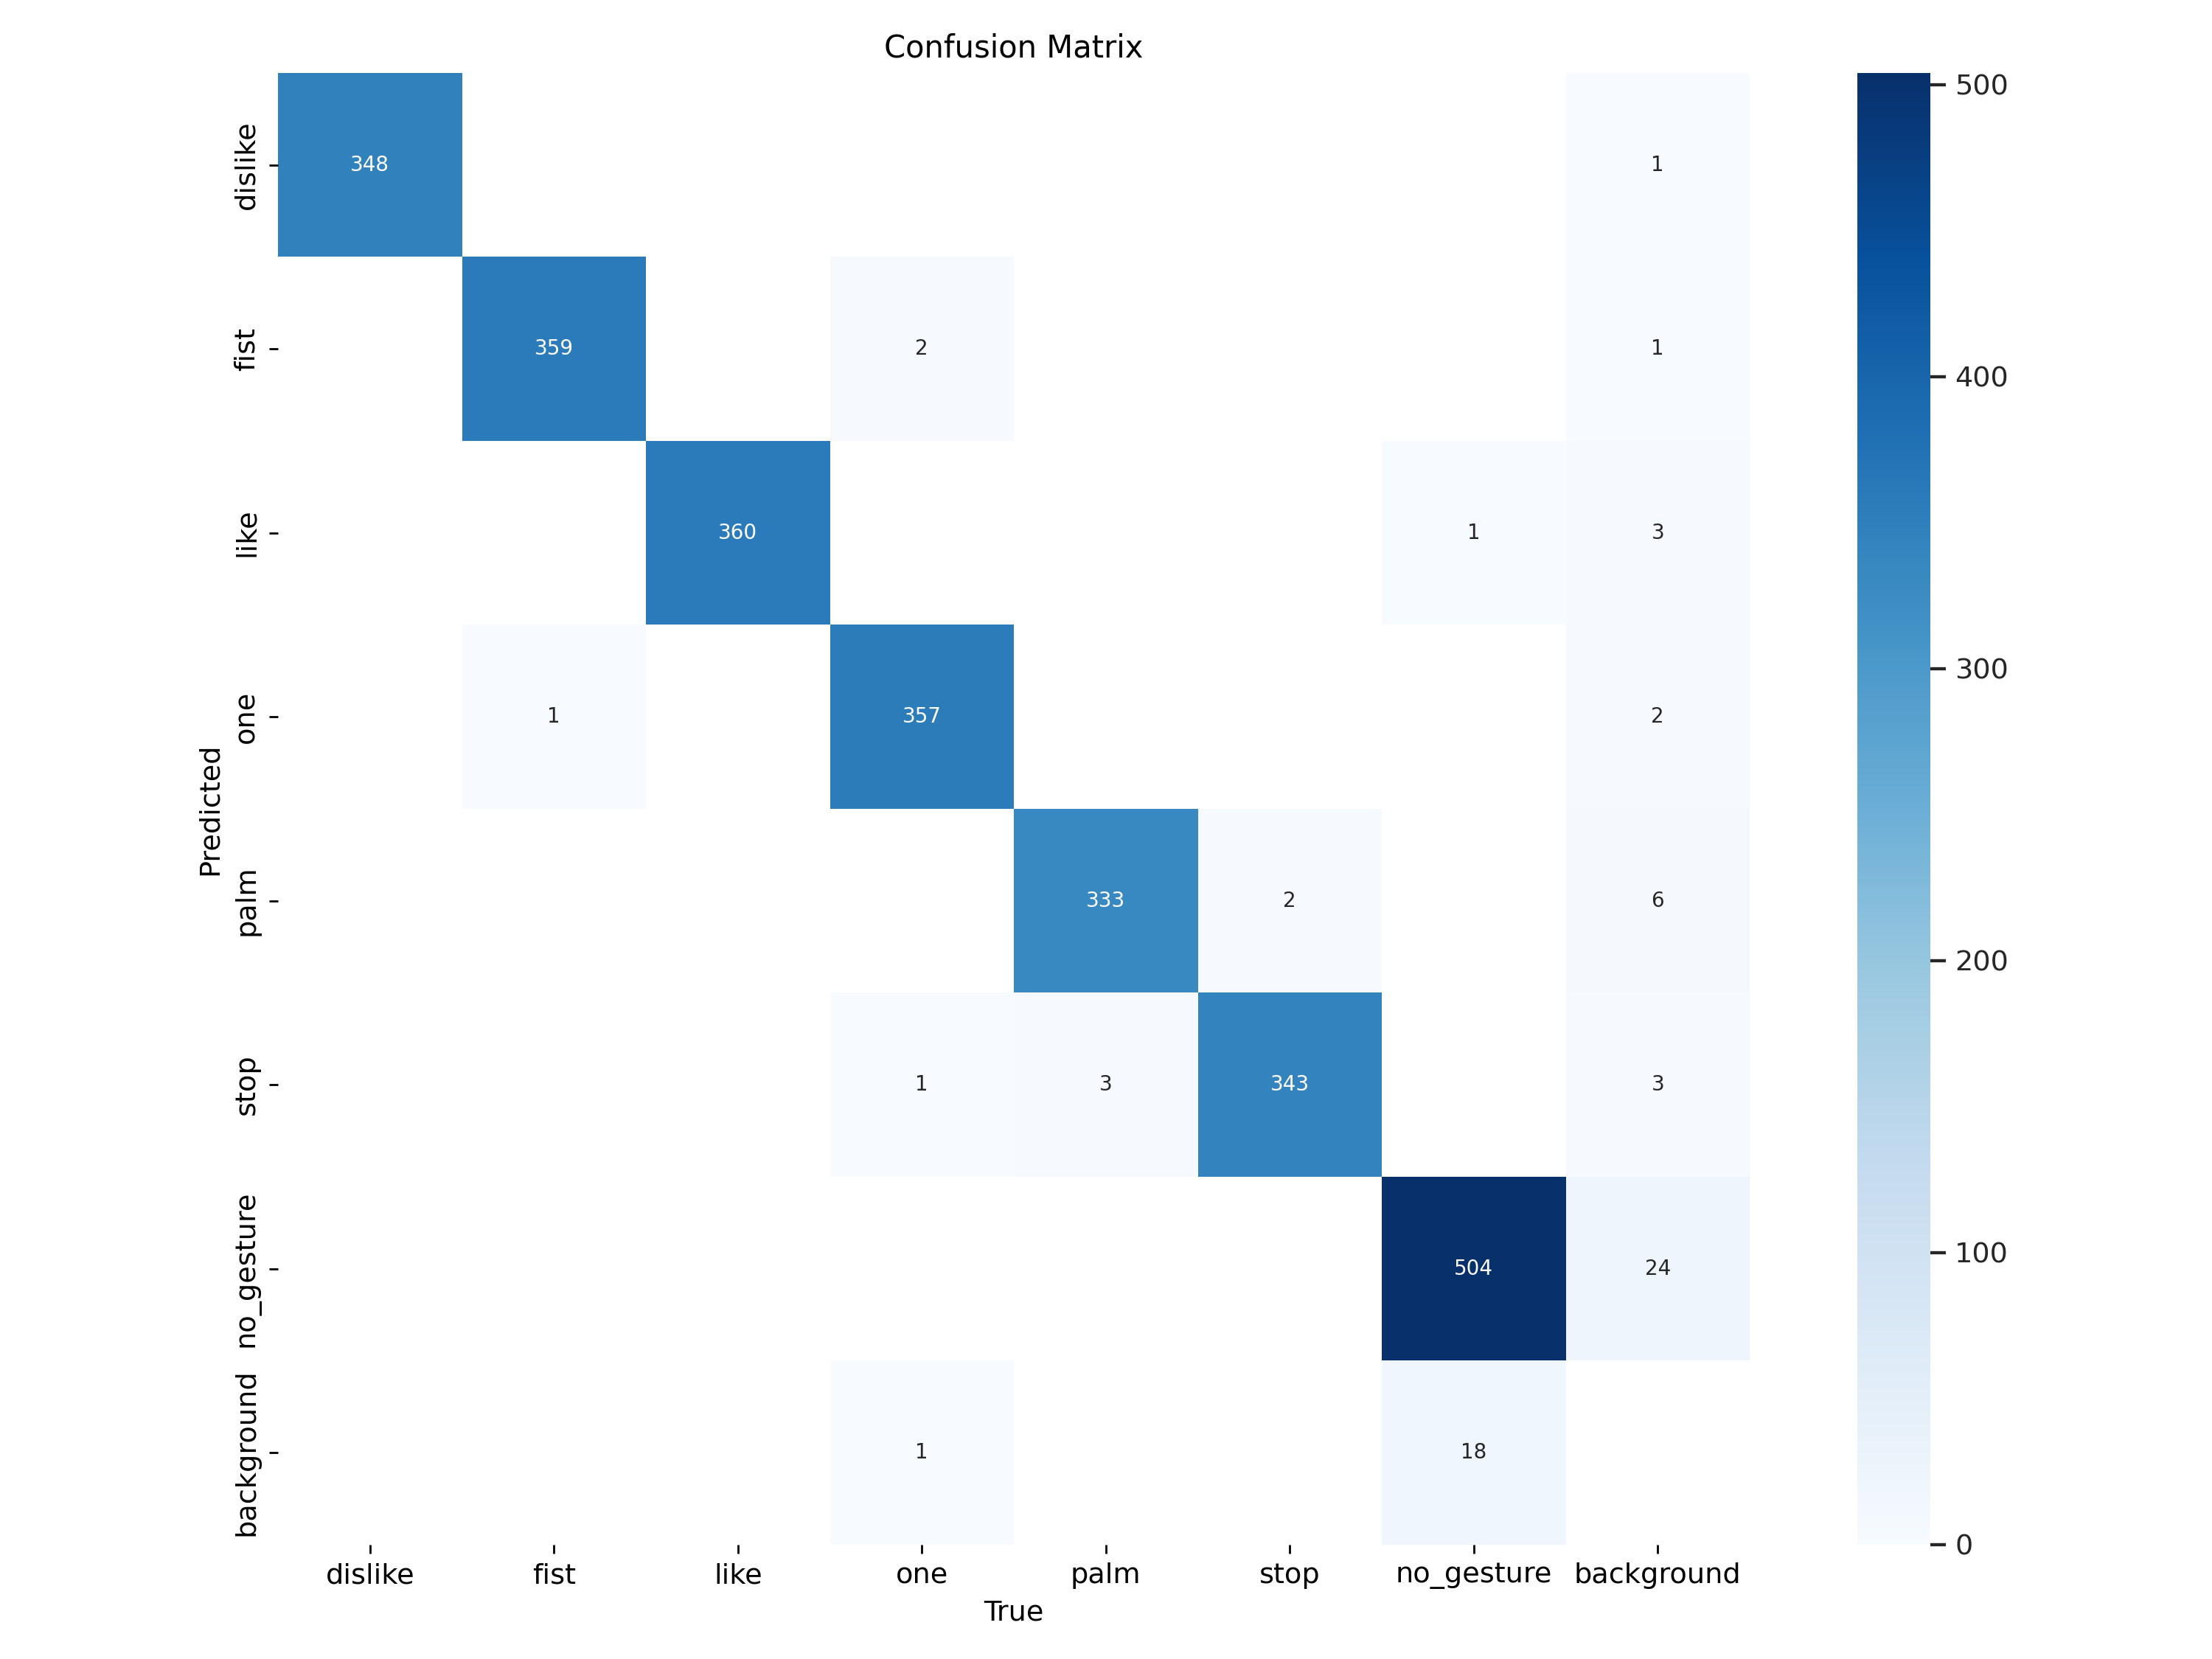
\includegraphics[width=0.475\textwidth]{./pictures/smallhands_confusion_matrix.png}
  \hspace{\fill}
  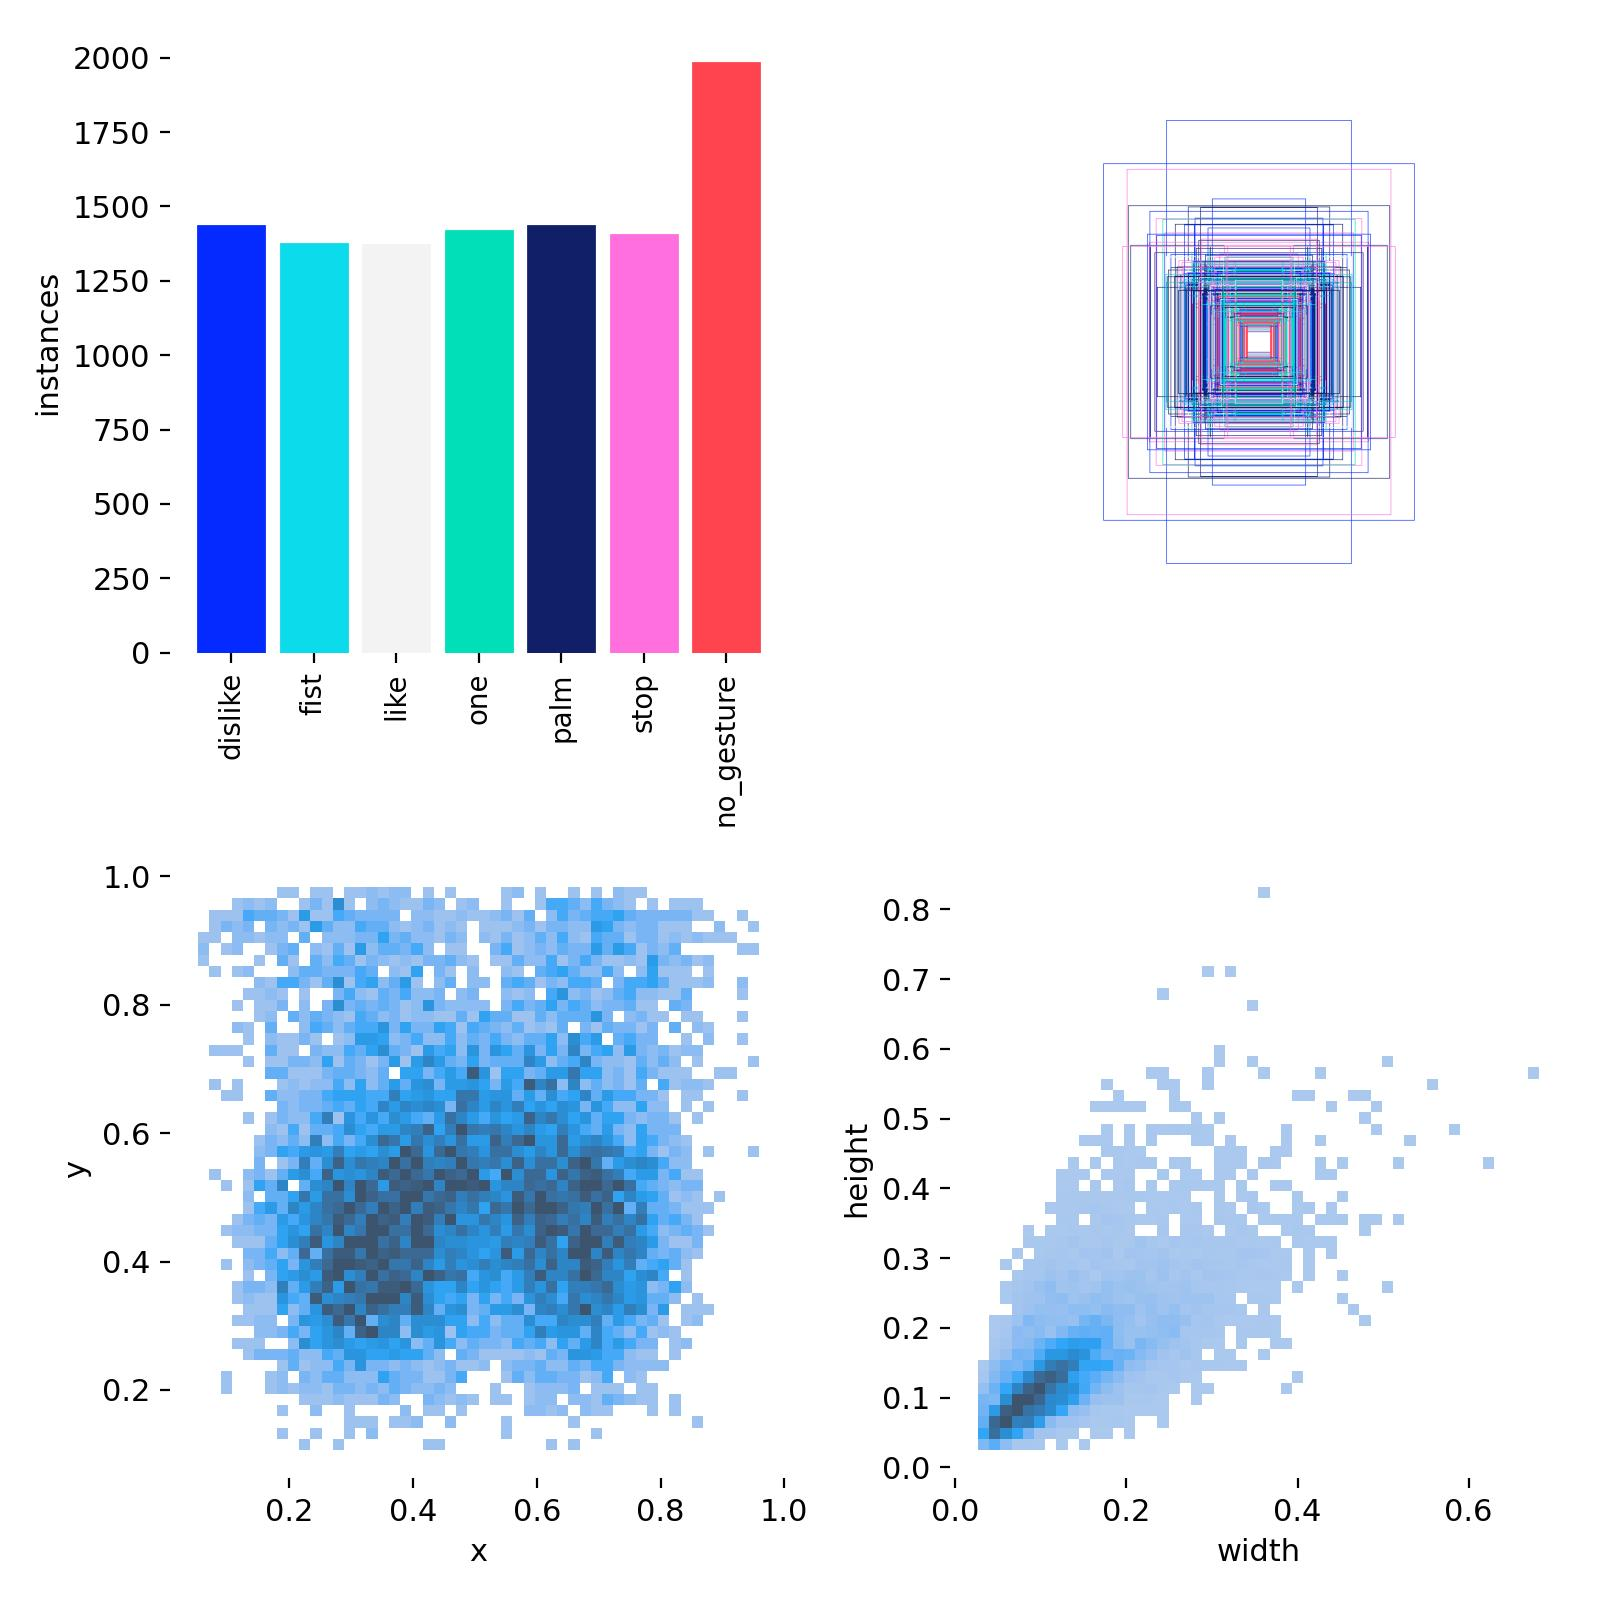
\includegraphics[width=0.475\textwidth]{./pictures/smallhands_labels.jpg}
  \caption{Confusion matrix on the left, and class distribution on the right of the HaGRID dataset. We can observe a relative balance between the classes, with the class "no\_gesture" being somewhat underrepressented. Overall, this shows that this dataset is well balanced and not prone to overfitting certain gestures over another. However, the lack of "no\_gestures" of different kinds makes it slighty prone to false positives (the dataset lacks hand gestures with two fingers up or so on, which is not supposed to trigger a detection.)}
\end{figure}

\begin{figure}[H]
  \centering
  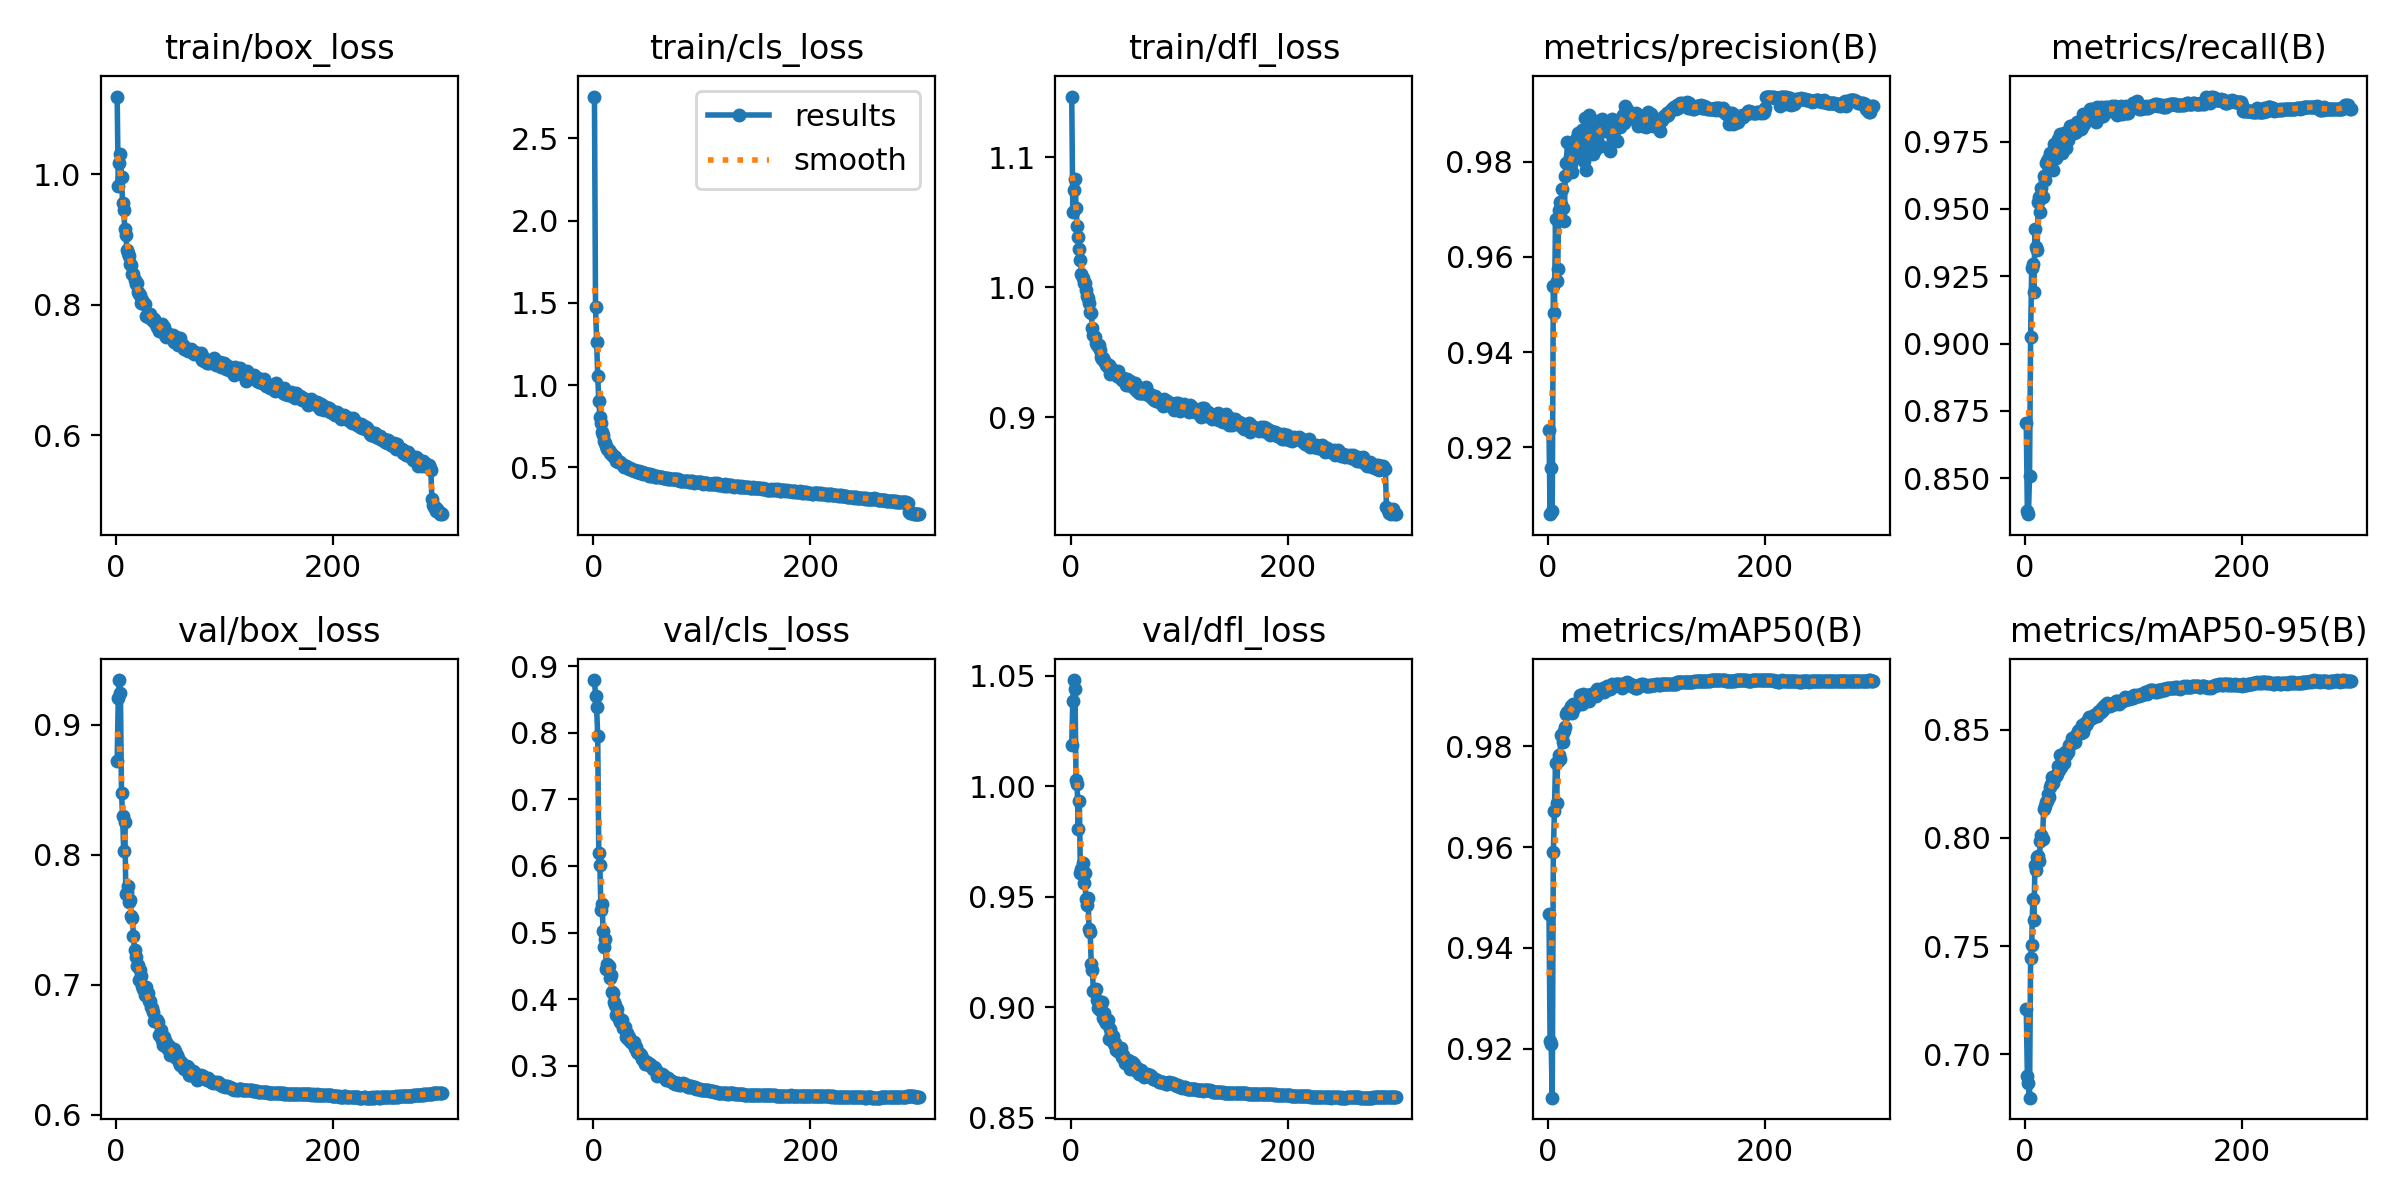
\includegraphics[width=\textwidth]{./pictures/smallhands_results.png}
  \caption{Training results ans metrics for the object detection model. The training did not stop early, as the validation loss kept decreasing over time, albeit in very small decrementations. We can also see that the metrics for this model quickly rose to above 0.99 for the mAP50 and to around 0.87 for the mAP50-95, meaning the model is extremely good and precise on the validation dataset.}
\end{figure}

\begin{figure}[H]
  \centering
  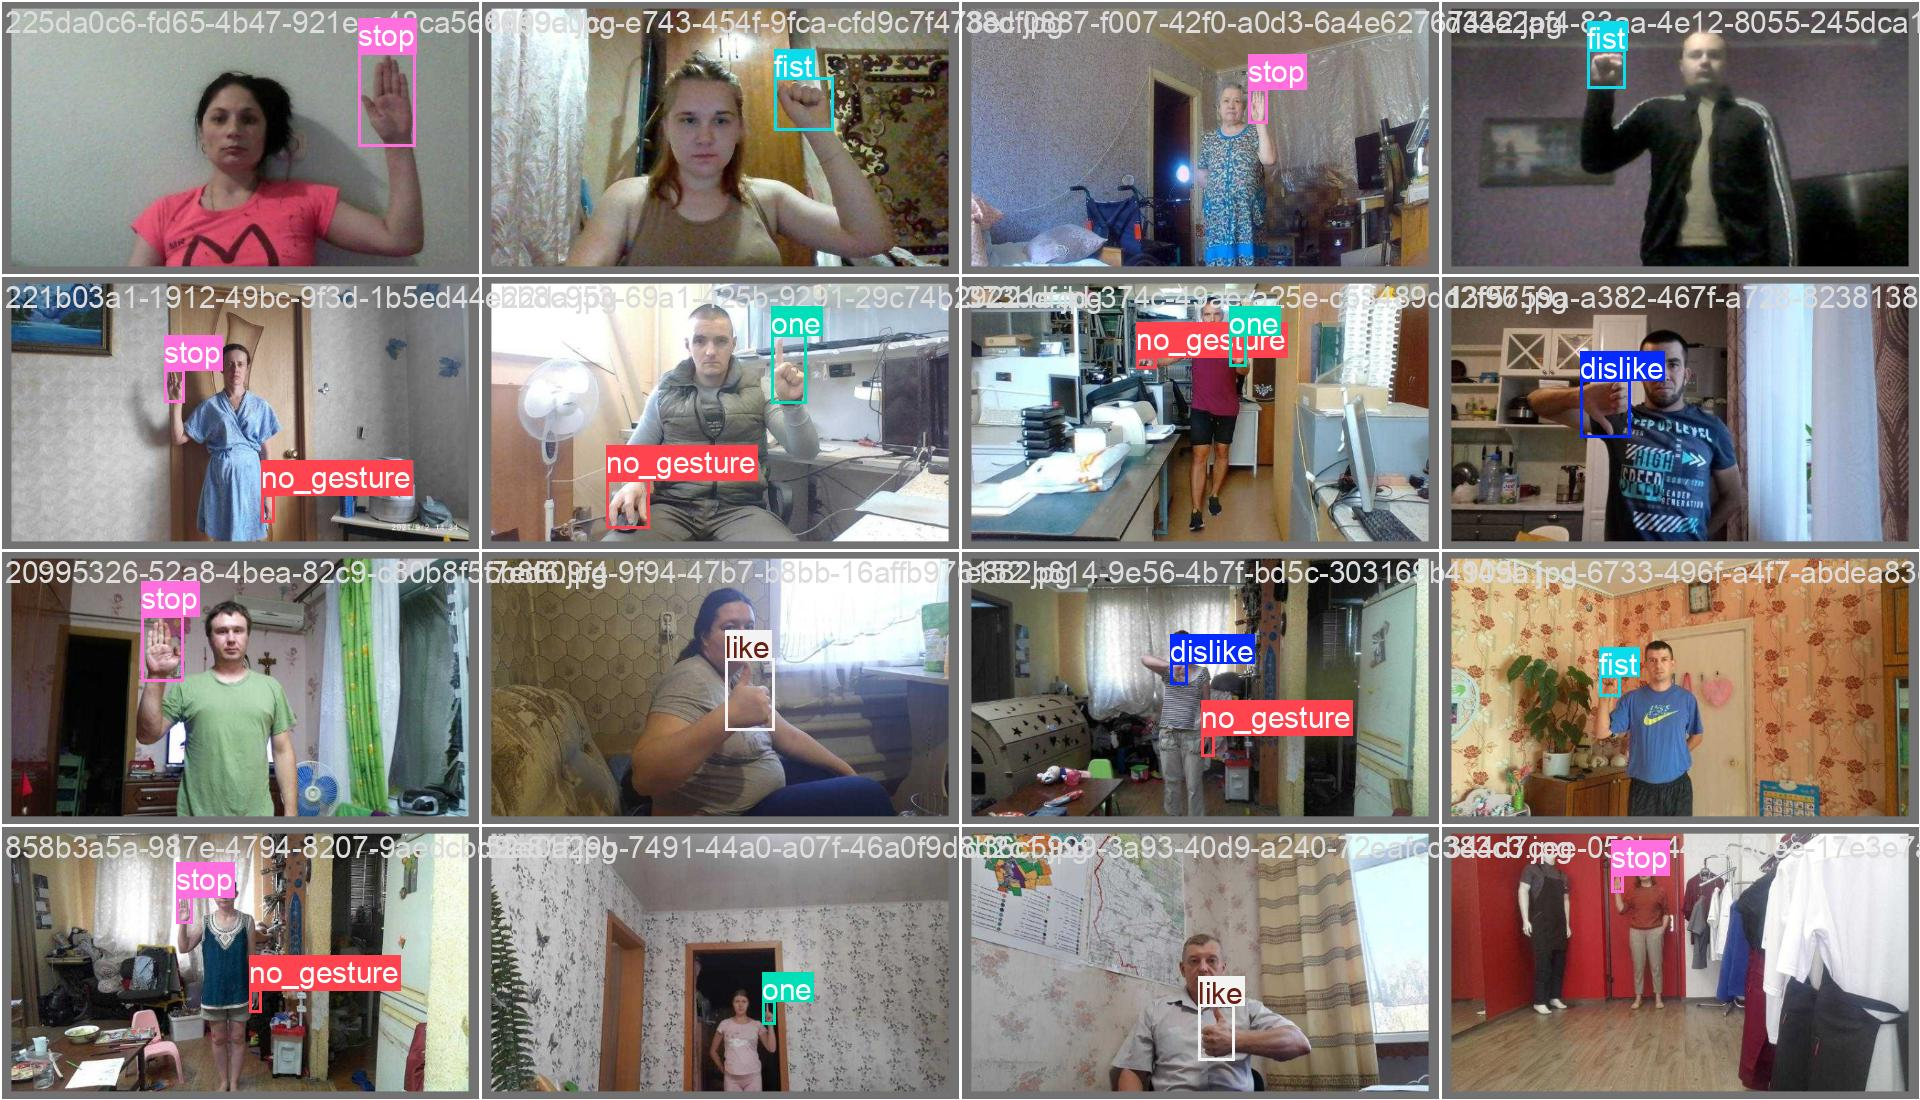
\includegraphics[width=0.475\textwidth]{./pictures/smallhands_batch_labels.jpg}
  \hspace{\fill}
  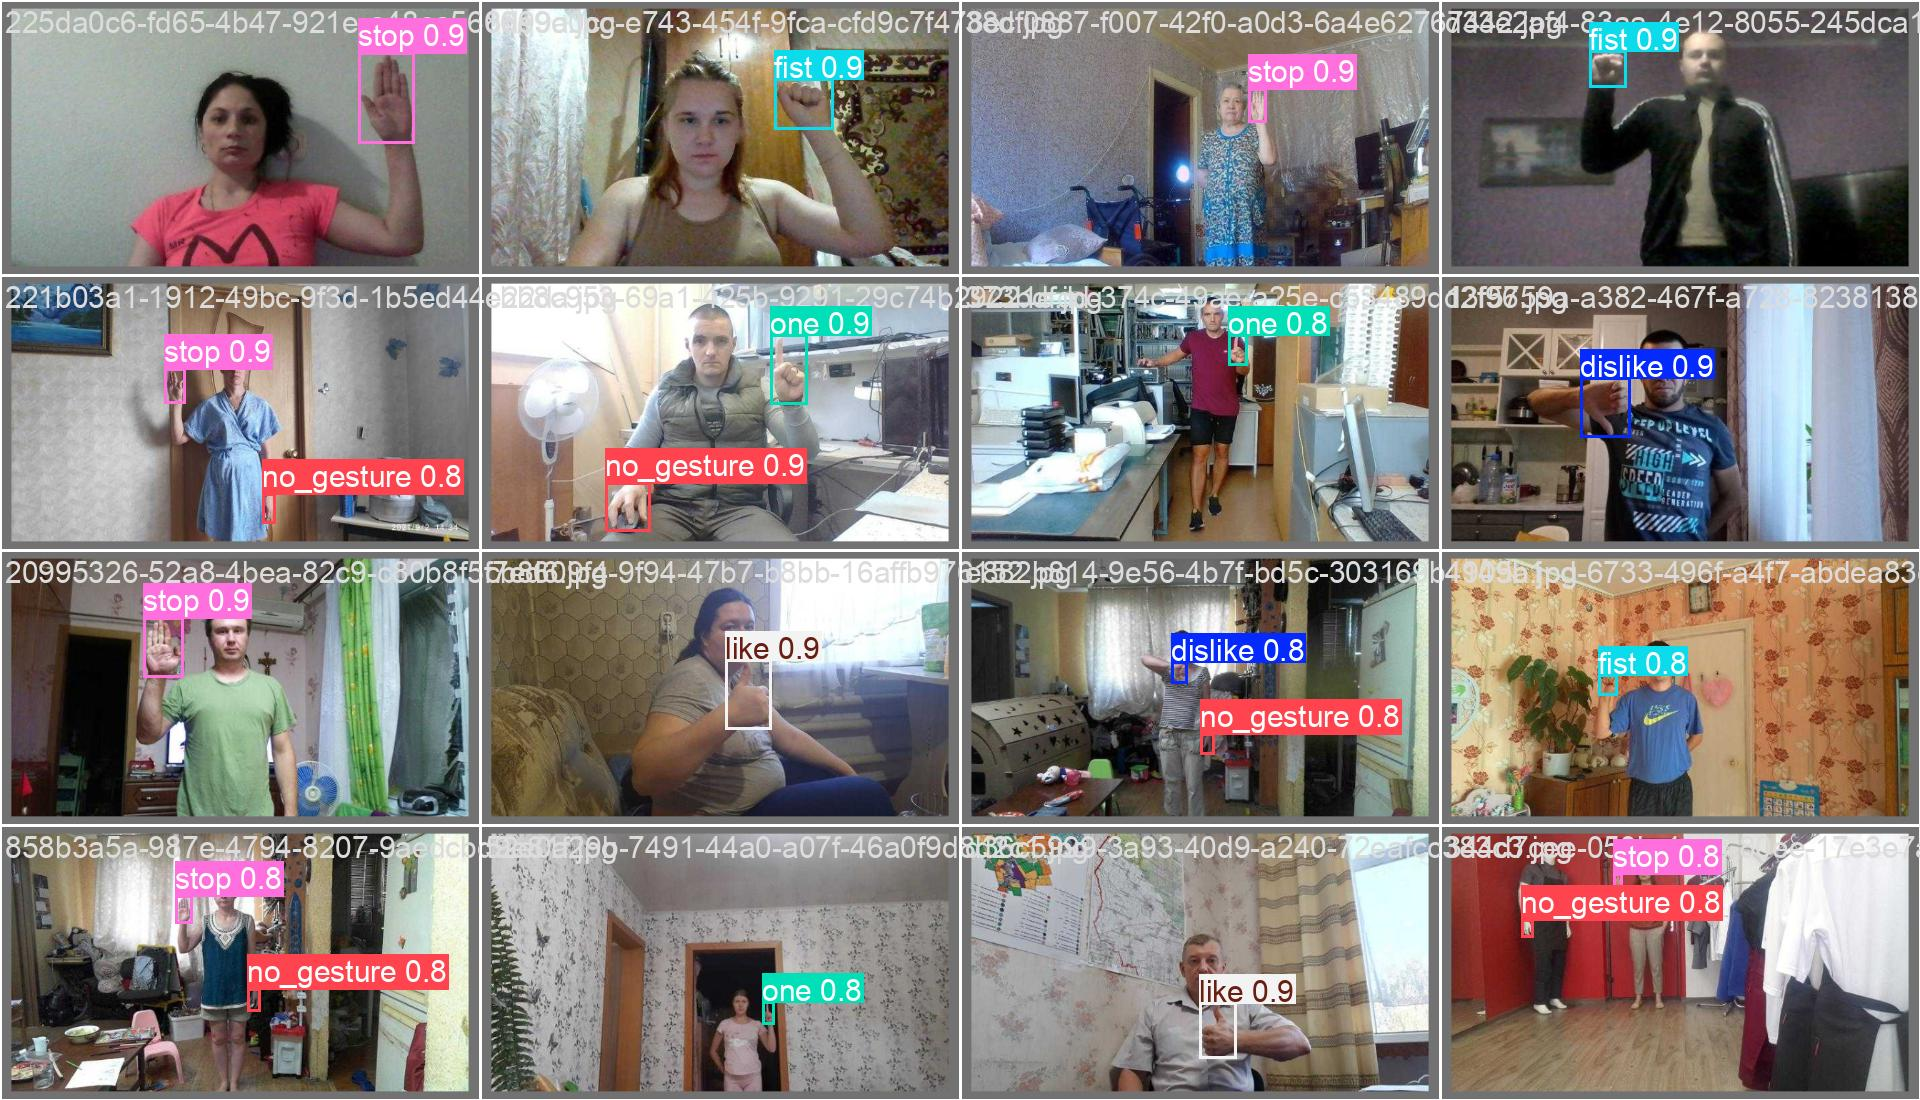
\includegraphics[width=0.475\textwidth]{./pictures/smallhands_batch_pred.jpg}
  \caption{Comparison between the ground truth values (left) and the predictions made by the fully-trained model. As we can see, this confirms the results previously obtained in the training metrics stating that the model is very precise.}\label{fig:xyz}
\end{figure}

Overall, the results for the object detection training are very promising, boasting an extremely high mAP50 and mAP50-95, which is to be expected when transfer learning on a very robust backbone model such as YOLO11. This detection technique, albeit simpler than pose estimation, should be more than enough to get accurate hand gesture readings from a video stream in real-time.

\subsubsection{Pose estimation}

\begin{figure}[H]
  \centering
  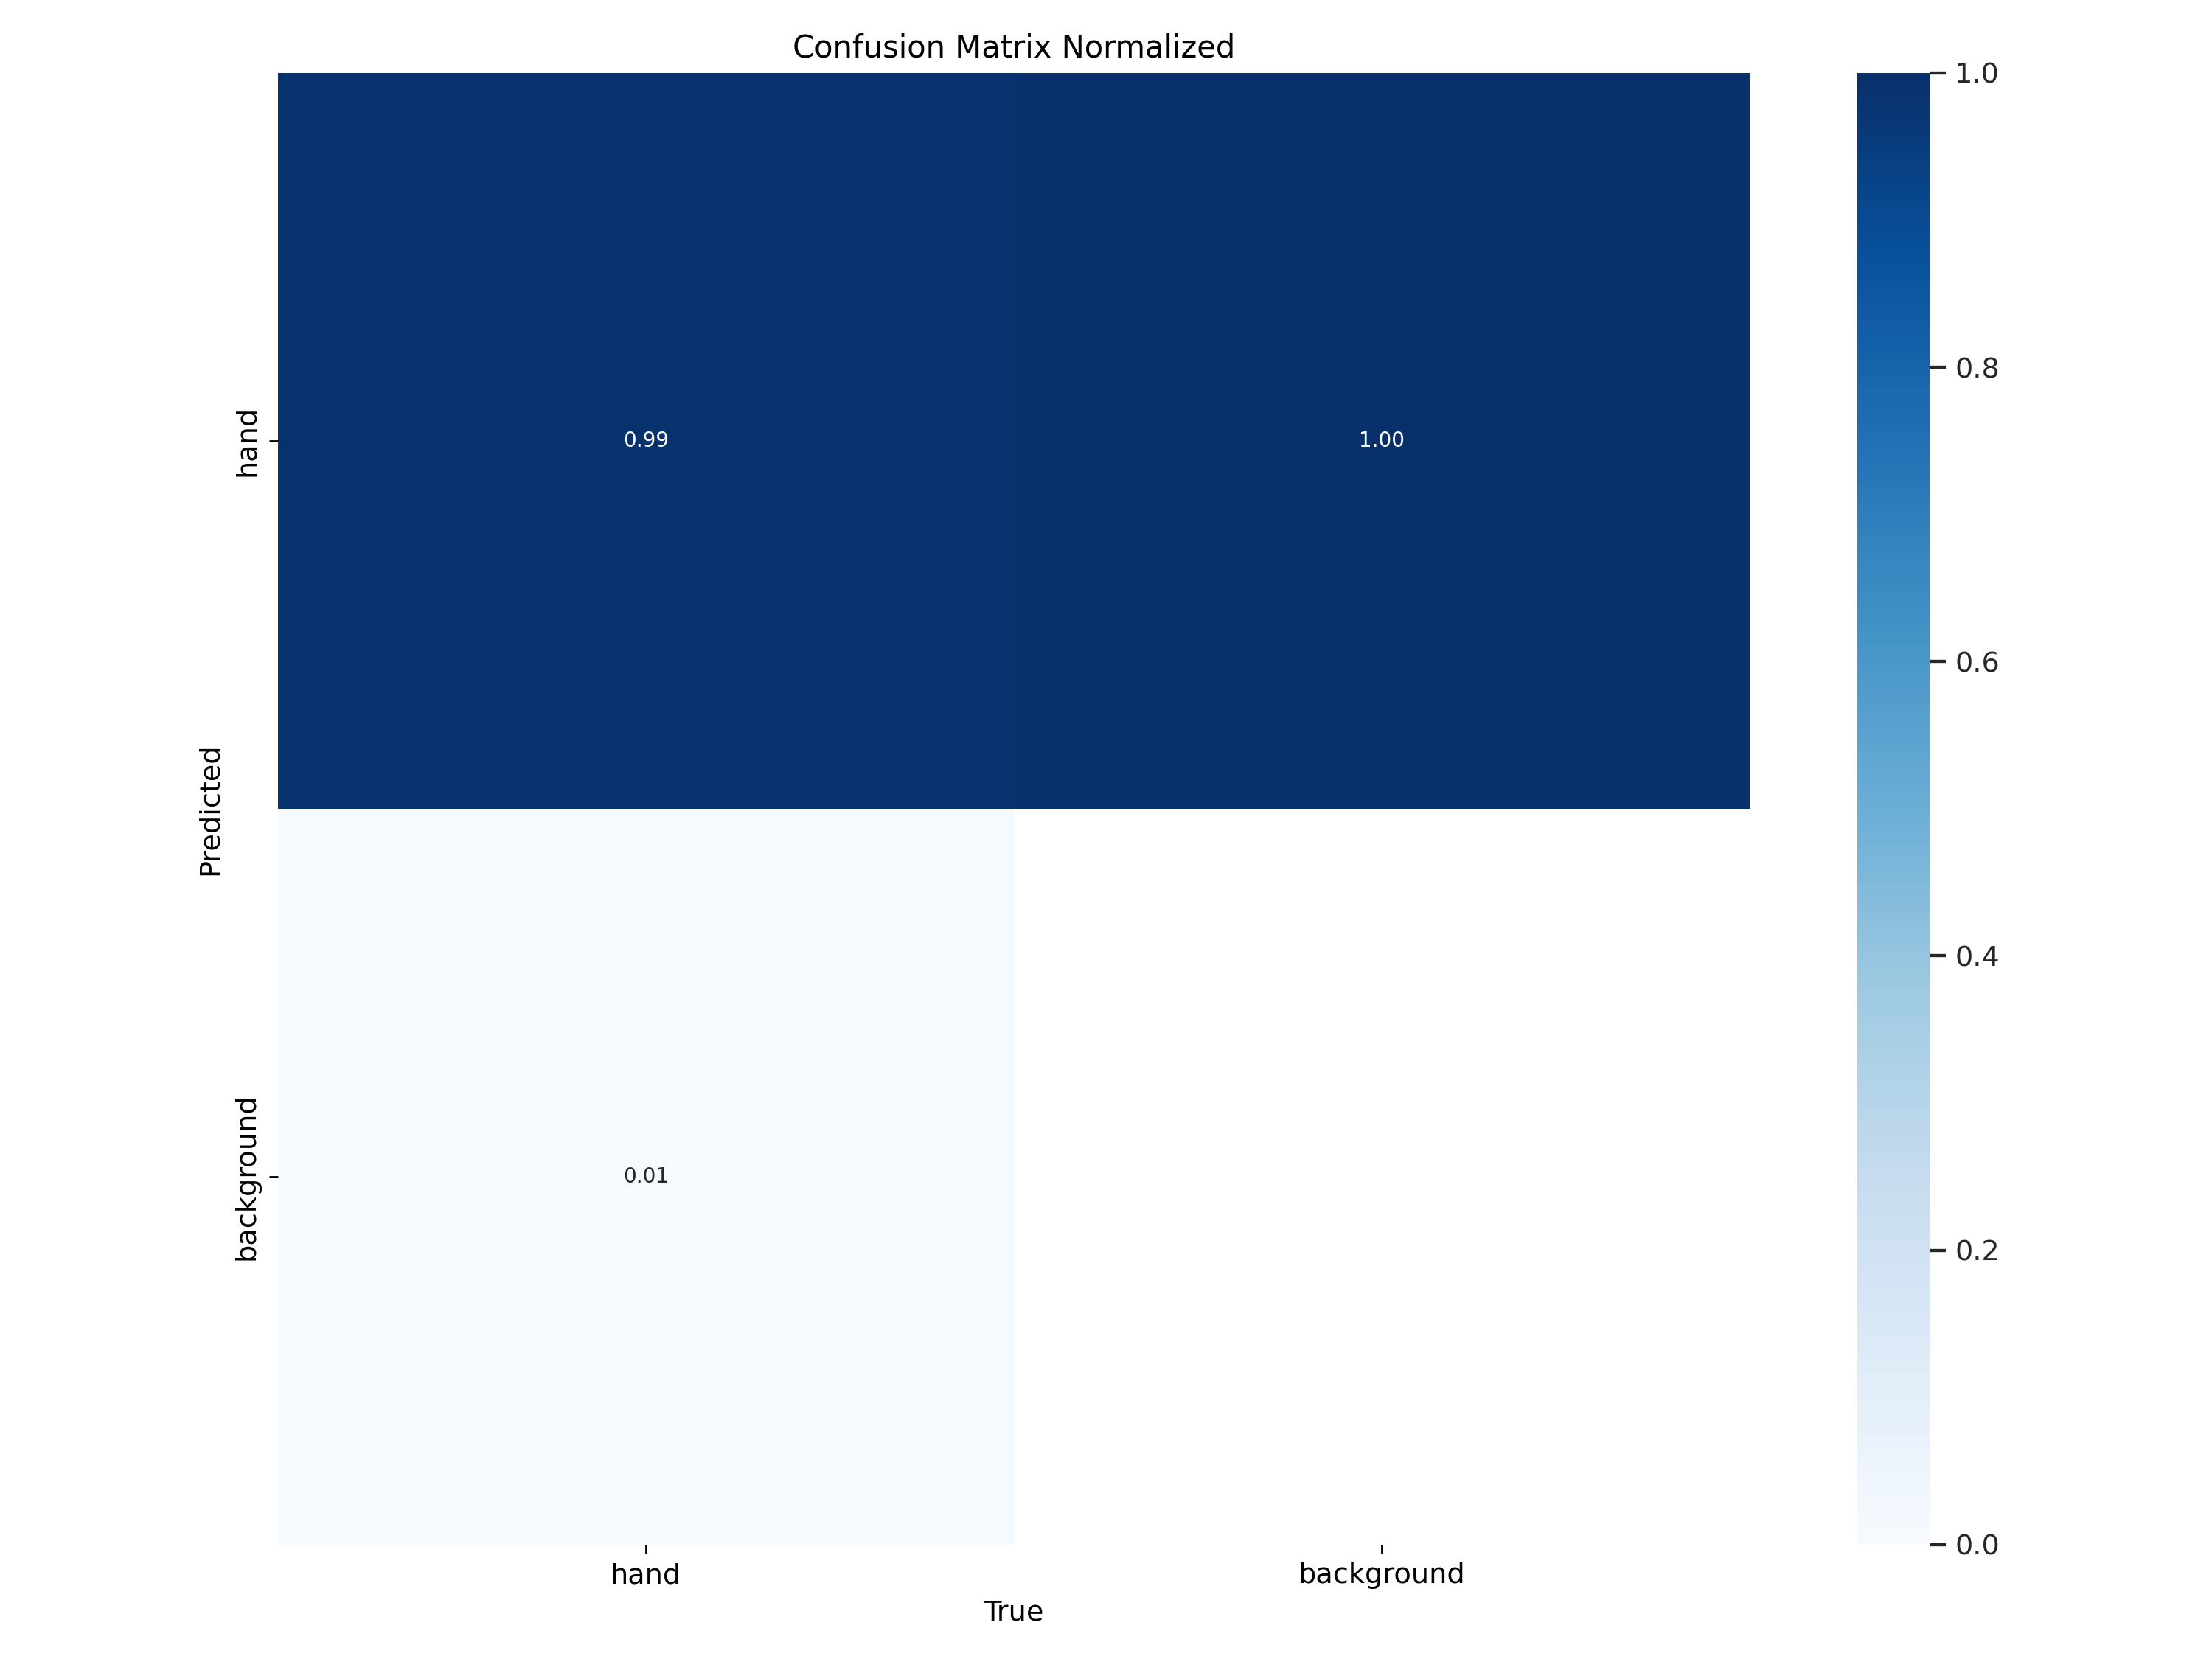
\includegraphics[width=0.475\textwidth]{./pictures/pose_confusion_matrix_normalized.png}
  \hspace{\fill}
  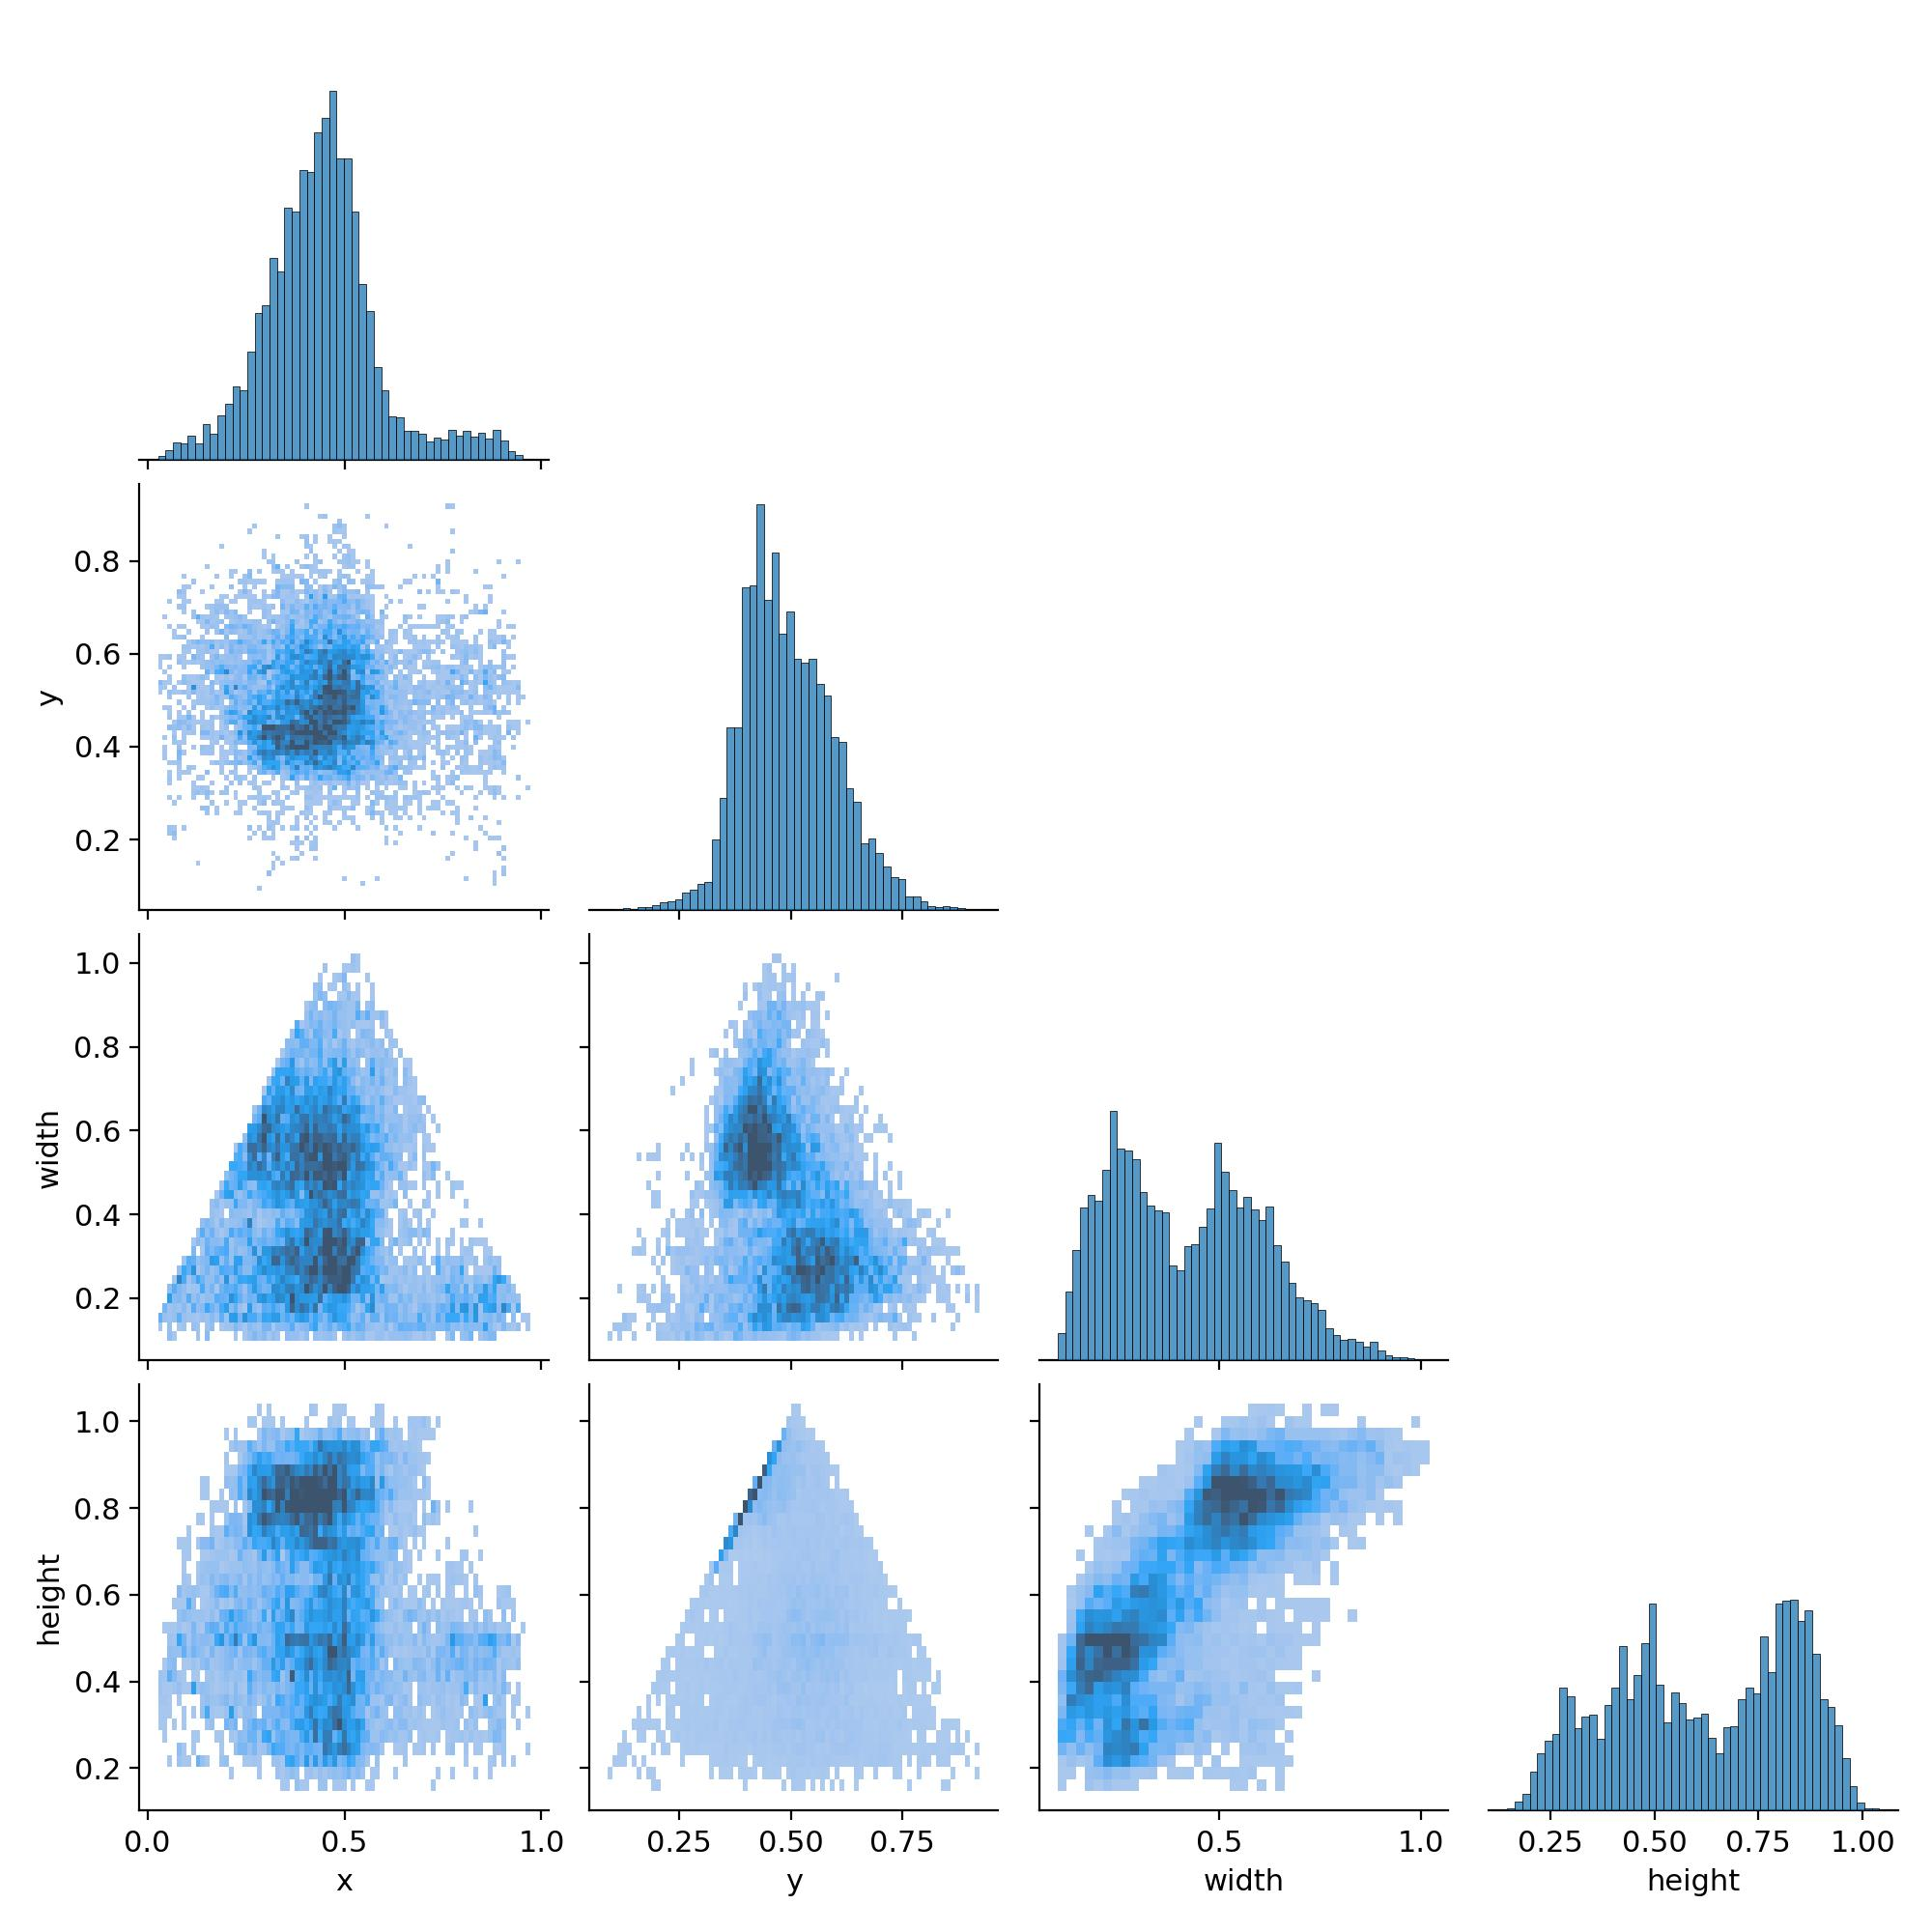
\includegraphics[width=0.475\textwidth]{./pictures/pose_labels_correlogram.jpg}
  \caption{Confusion matrix (normalized) of the pose estimation dataset (left), and the corresponding label correlalogram (right). While the confusion matrix doesn't tell much about the dataset (no particular classes and no bounding boxes, the hands are defined by 1 points), the label correlalogram tells us the position of the points is evenly distributed across the picture, showing that the dataset is diverse enough and shows hands in several different configurations.}
\end{figure}

\begin{figure}[H]
  \centering
  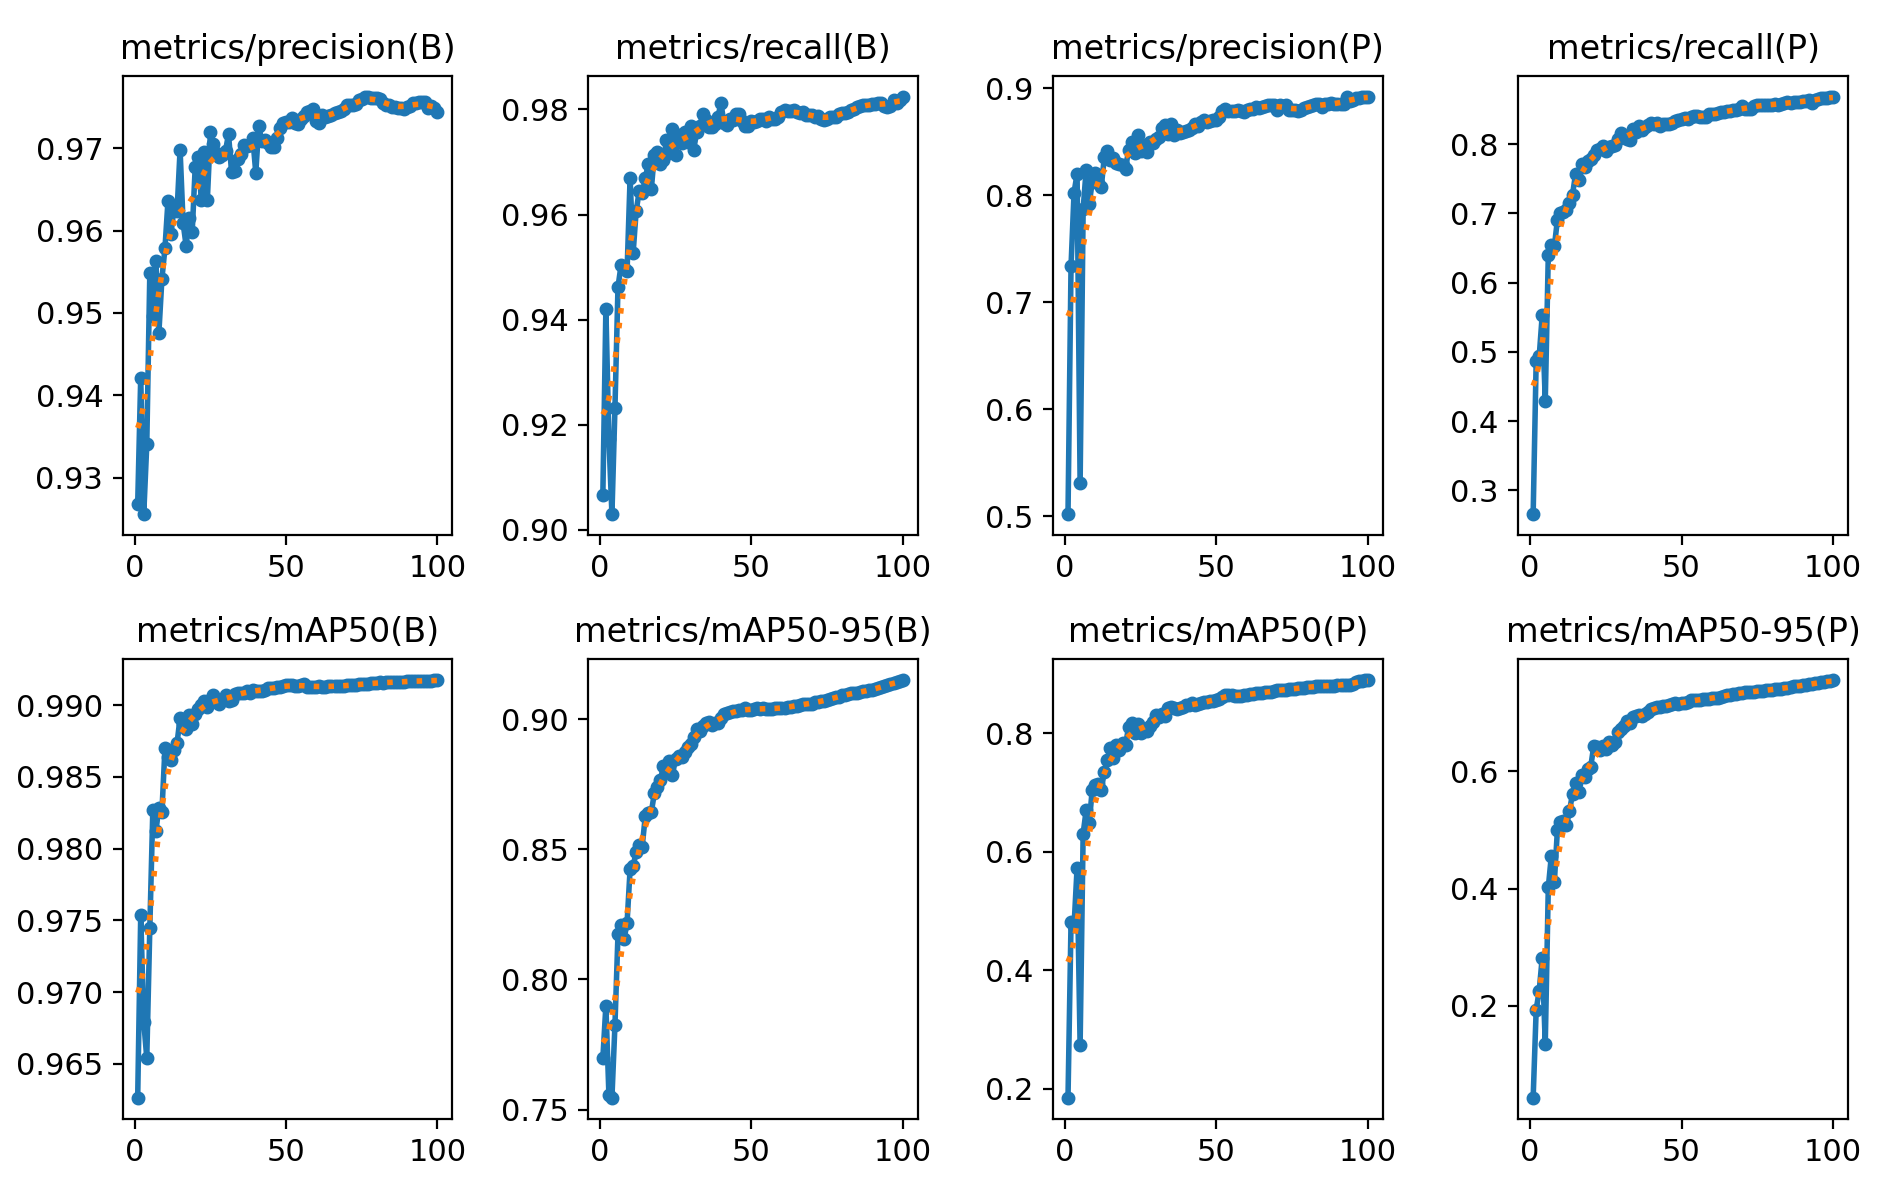
\includegraphics[width=0.7\textwidth]{./pictures/pose_results_metrics.png}
  \caption{Metrics results of the pose estimation training. Unsuprisingly, given the robustness of the YOLO backbone and the diverse dataset, the metrics kept incrementing over the epochs (with a bit of noise for the precision between the 20th and the 50th epoch). The pose estimation uses both bounding boxes and points for its metrics, the first one which is quite precise, even more so than the object detection for the mAP50-95 metric, going well above 0.90. However, since it's a more complex problem, the point metrics, which is how accurate the points placements tracking each joint is, are lower (0.8 for mAP50 and 0.75 for mAP0-95).}
\end{figure}

\begin{figure}
  \centering
  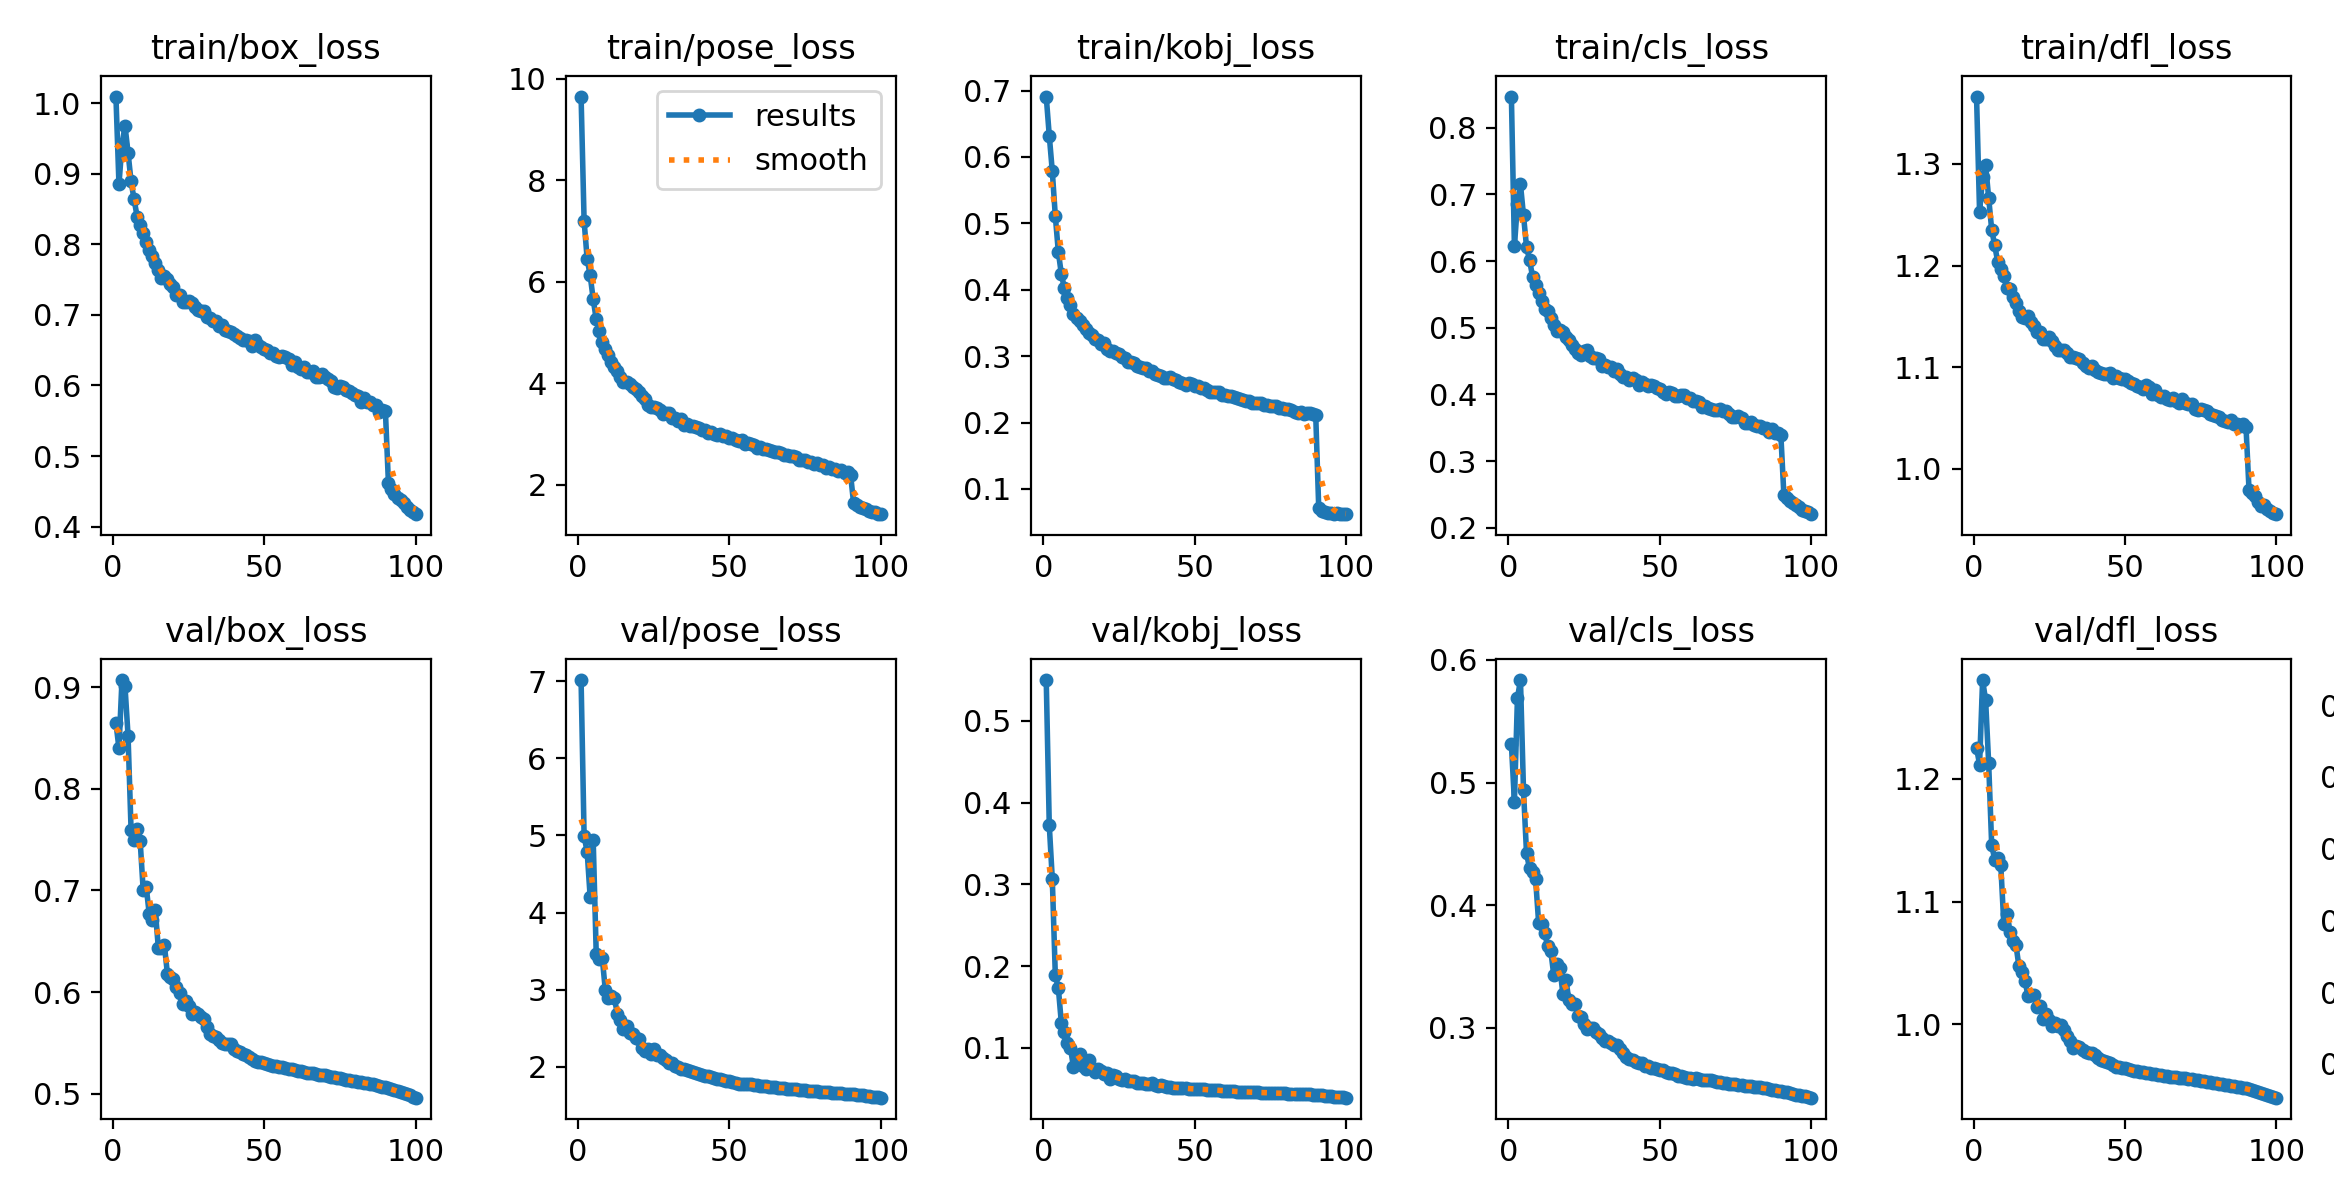
\includegraphics[width=0.7\textwidth]{./pictures/pose_results_losses.png}
  \caption{Loss results for the pose estimation training. Since the training ran its course without calling the early stopping callback, it is expected to see it gradually decrease over time. We can also notice a sharp decrease for the training losses at around the 80th epoch mark.}
\end{figure}

While the accuracy is slighty lower than the object detection technique, which is natural given the complexity of the task, the pose estimation detection model is also very robust in terms of accuracy and could also be used to detect very complex hand gestures, which shows more potential as a user interface for complex software.

\subsection{Benchmarks}

\subsubsection{Dell Latitude 7490 benchmarks results}

The tables containing the results of these benchmarks can be found on \hyperref[sec:benchmark]{Appendix 2}.

In the realm of hand gesture object detection, as we can assert on table \ref{table:oddl} at page \pageref{table:oddl} the results highlight PyTorch as the most compact format, with the smallest model size of 5.2 MB and achieving an impressive mAP50-95 of 0.8728. The inference time recorded was 84.97 ms per image, translating to a FPS of 11.77.
TorchScript, while offering a straightforward transfer from PyTorch, demonstrated an dramatic increase in model size, doubling it and reaching 10.4 MB, while decreasing marginally the mAP50-95 to 0.8688. Its inference time also worsened to 101.33 ms, yielding a lower FPS of 9.87. 
The ONNX format maintained a balance between model size and performance, with a size of 10.1 MB and identical mAP to TorchScript, but with a notable improvement in inference time of 66.71 ms leading to a higher FPS of 14.99, which is consistent with the format, whch boasts higher performance on CPU-focused environments.
OpenVINO derived the fastest inference time at 53.21 ms, achieving a peak FPS of 18.79, while aligning with other formats with a mAP50-95 at 0.8688, showing virtually no sacrifices on accuracy and precision. It was also marginally larger in terms of size, at 10.2 MB. Since the tests were ran on a Intel processor, OpenVINO achieving the best performance was expected.
PaddlePaddle showed significant shortcomings due to its large size of 20.2 MB, resulting in an extremely slow inference time of 253.86 ms and the lowest FPS of the group at 3.94.
MNN and NCNN offered comparable results in terms of mAP (both around 0.8688) and size (10.0 MB), with MNN having slightly better performance in inference time (72.77 ms for MNN and 98.61 ms for NCNN) and FPS (13.74 for MNN and 10.14 for NCNN) compared to NCNN.

Turning to the hand pose estimation results, we can see on table \ref{table:pedl} at page \pageref{table:pedl} the PyTorch format again emerged as the most compact model at 6.0 MB, but it exhibited a lower mAP of 0.7554. Inference time stood at 129.12 ms, giving it an FPS of 7.74.
Comparatively, the TorchScript format grew to 11.8 MB with a regression in mAP to 0.7398, while the inference time improved slightly to 112.90 ms, resulting in an FPS of 8.86.
The ONNX format was slightly smaller at 11.6 MB but had a similar mAP as TorchScript, with a more efficient inference time of 83.54 ms – reaching an improved FPS of 11.97.
OpenVINO again demonstrated its efficiency with the lowest inference time of 58.91 ms, yielding an outstanding FPS of 16.97 at the expense of larger model size (11.8 MB) and lower mAP (0.7398).
PaddlePaddle performed poorly in terms of FPS (3.69) and inference time (270.84 ms), despite being the largest model at 23.2 MB.
MNN and NCNN fell into a similar performance bracket; MNN had a size of 11.5 MB with slightly quicker inference performance (75.30 ms, 13.28 FPS) compared to NCNN's 11.6 MB size, 106.57 ms, and 9.38 FPS.

Overall, the OpenVINO format clearly stands out at being the fastest in inference time, without sacrificing precision and accuracy (in fact, they both remain extremely consistent overall, across every format, with a slight edge for the PyTorch format).
Both the ONNX and MNN formats did also much better than other alternatives, which is expected as they were explicitly made to perform better on CPU environments. 

The model size always staying under 12 MB, which could potentially be an issue for extremely constrained and niche situations (satellites, drones, compact tech), remains quite small, and it should not be an issue for most applications.

\subsubsection{Raspberry PI Model 4B benchmark results}

For the object detection benchmark on the Raspberry Pi, which can be found on table \ref{table:odrpi} at page \pageref{table:odrpi} PyTorch emerged as the most accurate and precise model, with an average mAP50-95 of 0.5399. The 5.2 MB model size suggests a lightweight implementation that efficiently utilizes the available memory on the Raspberry Pi. However, the inference time was relatively high at 136.20 ms per image, leading to a lower FPS of 7.34. This indicates that while PyTorch provides decent mAP performance, the latency could pose challenges for real-time applications where quick responsiveness is crucial.
TorchScript, though slightly heavier at 10.3 MB, had similar mAP performance of 0.5360. Its advantage was seen in the inference time, which dropped to 103.59 ms, allowing for a higher FPS of 9.65. This suggests improvements in speed over the standard PyTorch format, making TorchScript a viable option for cases where a slightly larger model size is acceptable in exchange for faster processing speed, which covers a lot of scenarios.
In stark contrast, the ONNX format, which is designed for interoperability, showcased an impressive reduction in inference time to 33.91 ms and achieved a commendable FPS of 29.49, despite having a model size of 9.9 MB and a mAP score of 0.5360. The ONNX format clearly stands out for its ability to combine reasonable accuracy with rapid inference capabilities, positioning it as a strong contender for real-time hand gesture detection on the Raspberry Pi.
OpenVINO, while being optimized for Intel architectures, also demonstrated superior performance with an inference time of just 27.41 ms and Fps of 36.49, maintaining the same mAP score of 0.5360 and a size of 10.2 MB. This indicates that the OpenVINO toolkit, primarily designed for edge devices, excels in optimizing the model for efficient processing, making it another excellent option for embedded systems.
On the opposite end of the performance spectrum, several formats like TensorRT, CoreML, and various TensorFlow formats (like TensorFlowSavedModel, TensorFlowGraphDef, and TensorFlowLite) failed the benchmarks, due to being GPU-focused exports formats. This is particularly notable for TensorRT and TensorFlow, which are primarily geared towards performance but fell short in this context. Their inability to yield workable models may stem from compatibility challenges with the architecture of the Raspberry Pi or the specific model used.
The results for PaddlePaddle and NCNN reveal some middle-ground performances. PaddlePaddle had a larger model size of 20.0 MB with a respectable mAP of 0.5360, but its inference time of 91.44 ms led to a lower FPS of 10.94, making it less efficient for real-time applications. On the other hand, NCNN with a 9.9 MB size and mAP of 0.5360 provided a decent inference time of 29.78 ms and an FPS of 33.58, making it suitable for applications needing a good trade-off between accuracy and inference speed.


For the pose estimation model on table \ref{table:perpi} at page \ref{table:perpi} surprisingly, the PyTorch format produced a size of 11.7 MB, with an mAP of 0.148, an inference time of 171.1 ms per image, and achieved a playback frame rate of 5.84 FPS. While functional, this model displayed the lowest accuracy among those that were successfully exported, indicating that even though it runs, its performance might not meet the demands of real-time applications.
The TorchScript format, although slightly smaller at 11.2 MB, showed a marked improvement in mAP at 0.215, yielding a reasonable inference time of 117.2 ms and getting a better FPS of 8.53. This suggests that TorchScript offers a good trade-off between compactness and performance, optimizing model responsiveness on the Raspberry Pi.
ONNX was an especially notable contender, with an almost identical size of 11.4 MB, maintaining the same mAP of 0.215, but dramatically improving the inference time to 37.9 ms and achieving an impressive FPS of 26.39. This suggests that ONNX is particularly well-optimized for the Raspberry Pi architecture, making it a viable candidate for real-time pose estimation tasks.
The OpenVINO also demonstrated commendable performance with an mAP of 0.215, a slightly higher model size (11.6 MB), and showcased excellent inference speed at 31.1 ms and 32.15 FPS, marking it as the fastest among those that successfully ran. The OpenVINO toolkit is explicitly designed for optimizing deep learning workloads on Intel hardware, which likely explains its superior efficiency on Raspberry Pi.
Moving on to TensorFlow models, the TensorFlowSavedModel was much larger at 28.8 MB, maintaining a solid mAP of 0.215; however, it had a slower inference time of 66.0 ms and 15.15 FPS, which indicates potential limitations in performing in a resource-constrained environment like Raspberry Pi.
In contrast, TensorFlowLite offers a more lightweight solution at 11.4 MB, displaying the same mAP of 0.215 and exhibiting slightly lower inference time (58.9 ms) and FPS of 16.98, making it another strong candidate for deployment. TensorFlow Lite is specifically designed to be an efficient version suited to mobile and edge devices.
The performance of models like PaddlePaddle (22.9 MB, mAP 0.215, 109.5 ms, and FPS 9.13) and both MNN (11.3 MB, mAP 0.214, 32.8 ms, FPS 30.49) and NCNN (11.3 MB, mAP 0.215, 33.5 ms, FPS 29.85) indicates a range of outcomes where MNN and NCNN match performances similar to ONNX and OpenVINO but with slightly heavier file sizes.
that prevent them from running on the Raspberry Pi environment, which is a crucial consideration when choosing a model for deployment.

In conclusion, surprisingly, the Raspberry Pi performs better than the mid-rangle laptop in terms of inference speed, while also making drastic sacrifices in accuracy. The OpenVINO seems to stand out as the most efficient export format in terms of inference speed, while not sacrificing accuracy when compared to other exports formats on the same task. The ONNX and the NCNN formats are also strong contenders, while the PyTorch format, while sometimes being marginally the most accurate, is very inefficient. In terms of storage space, the overwhelming majority of models falls under the 12MB range, and plays no role in terms of speed of accuracy, and should not hinder the deployment of such models on edge devices.

\subsection{Accuracy benchmarking}

The mAP50-95, while extremely helpful to gauge a model's effectiveness, does not tell us if a model can be used in real-world situations.

The mAP metric typically evaluates performance at a single Intersection over Union (IoU) threshold or an average across multiple thresholds. This might not reflect the model's true performance across all scenarios, as a model could still detect correctly a hand gesture while not necessarily predicting an accurate, or well-fitting, bounding box, reflecting in a low score.

On the flip side, the mAP may also not align with human interpretation of object detection accuracy, as it can yield high scores despite noticeable errors in visual quality or context.

Furthermore, the score also do not give or take into account penalties for overlapping detections. In some cases, predicted bounding boxes can overlap significantly without being penalized heavily, leading to high scores even in suboptimal situations.

In order to see in practice how accurate those models are, the object detection model and the pose estimate model will both be inferred on new data, using the OpenVINO format, as we found it to be the most promising candidate. The tests will be conducted on both the Dell Latitude and the Raspberry Pi.

Both models will be trained on two sets of data, the first one is a serie of 12 pictures of various hand gestures, taken with the Dell Latitude webcam at a small distance. The second set of data is a 30 seconds, 449 frames, 640x640 video displaying an user performing several hand gestures over the course of the video.

You may find the serie of the 12 pictures in \hyperref[sec:accuracy]{Appendix 3}, with the following :
\begin{itemize}
  \item The original dataset, on figure \ref{fig:predtest} at page \pageref{fig:predtest}.
  \item Results of the accuracy benchmark on the Dell Latitude, with the object detection benchmark on figure \ref{fig:objdell} and the pose estimation benchmark on figure \ref{fig:posedell}.
  \item Results of the accuracy benchmark on the Raspberry PI, with the object detection benchmark on figure \ref{fig:objrpi} and the pose estimation benchmark on figure \ref{fig:poserpi}.
\end{itemize}

\clearpage

\begin{table}
  \centering
  \begin{tabular}{ |p{5cm}|p{1.2cm}|p{2cm}|p{2cm}|p{2cm}|  }
    \hline
    \multicolumn{5}{|c|}{Benchmark results on the Dell Latitude} \\
    \hline
    Model&Data&Preprocess&Inference&Postprocess \\
    \hline
    Object detection&Images&2.7&47.0&0.8 \\
    Object detection&Video&3.1&46.9&1.1 \\
    Pose estimation&Images&3.7&51.5&3.0 \\
    Pose estimation&Video&3.5&57.1&1.4 \\
    \hline
  \end{tabular}
\end{table}

\begin{table}
  \centering
  \begin{tabular}{ |p{5cm}|p{1.2cm}|p{2cm}|p{2cm}|p{2cm}|  }
    \hline
    \multicolumn{5}{|c|}{Benchmark results on the Raspberry Pi} \\
    \hline
    Model&Data&Preprocess&Inference&Postprocess \\
    \hline
    Object detection&Images&9.4&312.4&2.7 \\
    Object detection&Video&10.8&307.0&2.9 \\
    Pose estimation&Images&9.7&370.3&4.0 \\
    Pose estimation&Video&10.7&360.2&4.0 \\
    \hline
  \end{tabular}
\end{table}

The benchmarking results of both the object detection and pose estimation models reveal an intriguing outcome: despite the inherent differences in processing power and hardware capabilities between a Dell laptop and a Raspberry Pi, both devices yielded identical predictions for both the video and the testing dataset, as seen in \hyperref[sec:accuracy]{Appendix 3}, which seems to contradict the performance metrics observed in the previous benchmark. This suggests that the models themselves are robust enough to perform consistently across varying hardware architectures, this also could be explained that these models were tested on the same export format, which was determined to be the most efficient in the previous benchmark : the OpenVINO export format.

For the tests performed on the Raspberry Pi, the inference time was significantly higher than expected. The inference time performace for the Dell Latitude was between 47ms and 57ms on average for the models on the Dell Latitude, which seems consistent to the results obtained for the OpenVINO in the previous benchmark. However, for the Raspberry Pi, the inference time performance average at 300ms, which is around ten times more than previously observed.

While the inference time is ten times worse than previously expected, the accuracy is the same as the models ran on the mid-range Dell Latitude laptop. The massive difference in inference time performance might be explainable by several factors.

Changes in lighting conditions, backgrounds, noise or object variations in the new data might cause a domain shift, and  can significantly impact performance. While the new data was of poor quality on purpose, it does not differ much from the training or validation data, so this is somewhat unlikely.

In some cases, running inference in a certain way (like batching inputs) might affect performance metrics. Testing the model on new data differently compared to how it was evaluated on validation data might affect both inference time and accuracy. Running the model on a single image might take longer if the model is optimized for batch processing where multiple images can be fed simultaneously.

In any case, those results seem to align more with reality and are therefore more suited to answer the research objective. But is a 300ms inference time fast enough for real-time application?

Real-time systems often operate under the criteria of being responsive enough for a user to interact with the system without noticeable delay/In most interactive systems, a response time of under 100ms is considered ideal for seamless interaction, such as gaming, full-body motion capture or remote control of IoT devices.

An inference time of 300ms means that there's a delay of three-tenths of a second before the system responds to a user's gesture. For applications like gaming, virtual reality (VR), or motion capture, this can feel sluggish, potentially ruining the user experience as users expect instantaneous feedback.

Some techniques exist in order to alleviate this, such as predictive algorithms that allow the system to anticipate user actions based on past gestures. However, this would also be more computationally intensive, which might harm the system more than it helps it.

Frame skipping, or only inferring on a few images a second instead of a video feed, might improve drastically the performance of the model. 

While a 300ms inference time is technically feasible for some simple applications, like interacting with basic software such as a media player, it is generally considered too slow for real-time hand gesture detection in intensive interactive settings. User expectations for responsiveness are typically much higher, especially in environments where immediate feedback is critical. For optimal performance, aiming for an inference time below 200ms or even below 100ms is advisable. 

\section{Discussion}

When assessing the performance of the same model across different hardware platforms, such as a mid-range Intel laptop and a Raspberry Pi, we observe notable discrepancies in accuracy. Specifically, the object detection model exhibited a significant decrease in accuracy of approximately 37.21\% when benchmarked on the Raspberry Pi, compared to its performance on the more powerful laptop. Even more striking was the pose estimation model, which showed a staggering accuracy decline of 70.95\%. Interestingly, despite these substantial drops in accuracy, the inference time on the Raspberry Pi was marginally faster than on the Dell Latitude laptop.

Several factors contribute to this phenomenon, primarily rooted in differences in the hardware capabilities of the two devices. One major consideration is thermal and power throttling; the Raspberry Pi tends to reduce its performance if it overheats or operates near its power limits. This can lead to slower processing times and a less effective utilization of computational resources, ultimately impacting the model's performance.

For these benchmarks, which were very CPU-intensive and ran for several hours, the Raspberry Pi reached criticals temperatures between 90-100 degrees Celsius, which might have hampered performance.

Furthermore, model compatibility plays a crucial role; models that perform optimally when trained on more powerful machines may struggle to adapt to the limited capabilities of the Raspberry Pi. Complex models, such as full YOLO or SSD architectures, may require simplification, including quantization or pruning, to run adequately on the Raspberry Pi, which often results in reduced accuracy.

Optimizations and quantization strategies also come into play. While employing lower precision formats, such as float16 or int8 in place of float32, can enhance inference speed on devices like the Raspberry Pi, this shift can compromise accuracy. The resolution of the input images fed into the model further complicates matters; if the Raspberry Pi handles resized or differently preprocessed images compared to the laptop, it can lead to diminished detection performance. Additionally, the chosen batch size during model evaluation significantly influences performance metrics. The Raspberry Pi may process images one at a time, contrasting with potentially larger batch sizes utilized on the laptop, thereby yielding different benchmarks.

Other considerations include the use of speed optimization techniques. These approaches, such as implementing early exit strategies in models or aggressive pruning, aim to speed up inference times on the Raspberry Pi but may inadvertently compromise the model's object detection accuracy by discarding essential features. In scenarios where the model is integrated into real-time or near-real-time applications on the Raspberry Pi, there is often a tendency to prioritize speed and responsiveness over accuracy, sometimes resulting in lower detection confidence thresholds to maintain quicker processing rates.

The significant differences in accuracy and inference times observed when comparing a Raspberry Pi to a laptop stem from a multitude of factors related to hardware limitations, model configurations, software variations, and processing efficiency. Achieving optimal performance on edge devices necessitates a careful balancing act between speed and accuracy, which may involve employing different model architectures or preprocessing strategies customized for the constraints of the Raspberry Pi. To enhance performance in such environments, it is advisable to consider utilizing lighter models specifically designed for edge computing, applying quantization techniques judiciously, and conducting comprehensive testing under controlled conditions to ascertain the models' effectiveness.

\section{Conclusion}

Deep learning has emerged as a highly promising approach for hand gesture recognition, significantly outperforming traditional techniques. With its ability to automatically learn complex patterns from large datasets, deep learning models, especially robust convolutional neural networks (CNNs) such as YOLO11, excel at processing visual information and extracting nuanced features. Unlike classical methods that often rely on handcrafted features and simplistic models, deep learning leverages the vast amounts of data available in the form of images and videos, allowing for more robust and accurate gesture recognition. This capability is particularly beneficial in dynamic environments, where variations in lighting, orientation, and background can pose challenges. Additionally, deep learning methods can adapt to new gestures through transfer learning, reducing the need for extensive retraining. The superior performance of deep learning in recognizing subtle distinctions between gestures and its scalability makes it an invaluable tool in applications ranging from human-computer interaction to sign language translation and virtual reality. Overall, the advancements in deep learning technology signal a transformative shift in hand gesture recognition, setting a new standard that outmatches traditional techniques.

When it comes to real-time hand gesture recognition on edge devices, the choice between object detection and pose estimation is critical, particularly considering the constraints of computational resources and the need for rapid processing. Object detection is often favored because it is typically less computationally intensive and can quickly identify and classify gestures by recognizing the overall shape and location of the hand within a specific frame. With current advancements as demonstrated by YOLO11 by Ultralytics, object detection systems can provide efficient and accurate results with lower latency, making them suitable for devices with limited processing power. 

On the other hand, pose estimation, which involves analyzing the precise positions of hand joints and their spatial relations, requires more intensive computation and a higher level of detail. While pose estimation offers improved accuracy for complex gestures, its demand for intricate calculations may lead to delays, potentially compromising the real-time responsiveness essential in interactive applications. Given that edge devices often operate in dynamic environments with variable lighting and occlusions, the robustness and efficiency of object detection make it a more viable choice for seamless hand gesture recognition, enabling users to interact intuitively without experiencing noticeable lag. This strategic selection underscores the importance of balancing accuracy, responsiveness, and the specific capabilities of edge computing when developing gesture recognition systems.

Batch processing in vision-based deep learning hand gesture recognition can offer significant speed advantages during the training phase, as it allows for the simultaneous processing of multiple input images or video frames. This method takes advantage of vectorized operations (which is even more efficient on GPU-focused environments) leading to more efficient use of computational resources and reduced training times. However, when it comes to real-time applications, batch processing is inherently ill-suited due to its fundamental operational structure. In real-time scenarios, immediate feedback and responsiveness are critical; users expect instantaneous gesture recognition without any perceptible delay. Batch processing, by nature, involves collecting and processing inputs in groups, which introduces latency as the system waits to accumulate sufficient data before performing analysis. This batching delay can disrupt the fluidity of interactions, leading to a disjointed user experience where gestures may be recognized too late to be relevant. Moreover, the variability in how gestures are performed, each individual may have subtle differences in speed and style, can further complicate the batch processing approach, making it less adaptable in dynamic environments. Consequently, although batch processing excels in training scenarios for speed and efficiency, its inherent latency and inflexible handling of input data make it unsuitable for the real-time requirements of hand gesture recognition systems.

Deep learning hand gesture recognition models can indeed achieve performance suitable for simple software applications when running on devices like the Raspberry Pi 4B, averaging around 300 milliseconds per inference. This relatively low latency can enable basic gesture control functionalities, such as interacting with smart home devices or navigating user interfaces on simple applications. However, while frame skipping strategies—where the model processes only a subset of input frames, allowing it to maintain a perceived real-time interaction—can enhance the responsiveness of the application, the Raspberry Pi 4B may struggle under more demanding conditions. Applications requiring a higher frame rate or lower latency, such as real-time video gaming, augmented reality, or complex robotic control, would find the 300ms performance inadequate. In contrast, alternative low-power devices such as NVIDIA Jetson Nano or Google Coral Dev Board often feature more powerful GPUs and TPUs, respectively, which are tailored for accelerated deep learning tasks. These devices can handle more intensive computational loads and provide faster inference times, making them better suited for robust, real-time gesture recognition applications that involve higher frame rates or more complex model architectures. As the demand for more responsive systems increases, developers might opt for these alternatives to achieve the necessary performance for advanced interactive experiences.

\subsection{Recommendations}

Further research into the relationship between the distance between the user and the camera and image resolution in the context of vision-based deep learning hand gesture recognition is essential for optimizing system performance and practicality. As image resolution increases, the detail captured within the frame also increases, potentially enhancing the accuracy of gesture recognition algorithms; however, larger imagery may introduce challenges such as increased computational load and latency, which could negatively impact real-time performance. Conversely, capturing gestures from a greater distance may allow users to interact with smart home devices more comfortably, promoting accessibility and user experience. This research could explore the trade-offs between image quality and the operational distance, examining how different resolutions at varying distances impact classification accuracy, processing times, and overall system usability. Understanding these dynamics holds promise for developing robust hand gesture recognition systems that seamlessly integrate into smart environments, thus paving the way for more intuitive and user-friendly technological interactions.

Researchers and developers should consider exploring more powerful edge devices beyond the Raspberry Pi 4, such as the Google Colab Dev Board and the NVIDIA Jetson series. These devices offer enhanced computational capabilities and specialized hardware optimizations that can significantly improve the efficiency and accuracy of gesture recognition models. The Google Colab Dev Board provides an easy-to-use environment with scalable resources, which can facilitate rapid prototyping and testing of various model architectures. Meanwhile, the NVIDIA Jetson platform, equipped with powerful GPUs, enables real-time processing and the ability to handle complex neural networks that are essential for high-performance gesture recognition tasks. Furthermore, investigating the potential of Tensor Processing Units (TPUs) could prove to be particularly interesting, as these specialized hardware accelerators are designed for high-throughput and low-latency inferencing, making them ideal for machine learning applications. Implementing studies that test these advanced edge devices could lead to significant advancements in the efficiency and applicability of hand gesture recognition systems across various domains, including robotics, augmented reality, and human-computer interaction. This line of research not only promises to enhance the performance metrics of gesture recognition systems but also to broaden their accessibility and deployment in real-world environments, paving the way for more intuitive and responsive user interfaces.

Overall, future research should focus on benchmarking more deep learning detection models on several devices, instead of focusing on accuracy score. As the inference time is crucial for edge devices for real-time applications, the lack of data on these subjects is concerning and it would greatly benefit developers and help them explore new ventures in human-computer interfaces.

\clearpage

\section{Appendix 1 : Hardware specifications}

\subsection{Dell Latitude 7490}

Processor : Intel® Core™ i5-8350U Processor, with four cores and 8 threads, running at a maximum frequency of 3.60 Ghz and at an average of 1.70 GHZ, with a TDP of 15 watts.

Memory : 8 GB

Graphics : Intel UHD Graphics 620

Webcam : Integrated full HD webcam

\subsection{Raspberry PI 4B}

Processor : Broadcom BCM2711, Cortex-A72 64Bit SoC, running at 1.80 GHz, with a TDP of 3A@5V

Memory : 4 GB

Graphics : Videocore VI at 500Mhz

Webcam : Raspberry PI 5MP sensor board, with a native resolution of 5 megapixels, and has a fixed focus lens onboard. In terms of still images, the camera is capable of pictures with a resolution of 2592 x 1944 pixels, and also supports 1080p30, 720p60 and 640x480p60/90 video.

\clearpage

\section{Appendix 2 : Benchmark results}
\label{sec:benchmark}

\begin{table}[H]
  \centering
  \begin{tabular}{ |p{3cm}|p{2cm}|p{2cm}|p{3cm}|p{2cm}|  }
    \hline
    \multicolumn{5}{|c|}{Object detection on Dell Latitude 7490} \\
    \hline
    Format& Size(MB) &mAP50-95(Box) &Time (ms/instance) &FPS\\
    \hline
    PyTorch&5.2&0.8728&84.97&11.77 \\
    TorchScript&10.4&0.8688&101.33&9.87 \\
    ONNX&10.1&0.8688&66.71&14.99 \\
    OpenVINO&10.2&0.8688&53.21&18.79 \\
    TensorRT&0.0&NaN&NaN&NaN \\
    CoreML&0.0&NaN&NaN&NaN \\
    TensorFlow SavedModel&0.0&NaN&NaN&NaN \\
    TensorFlow GraphDef&0.0&NaN&NaN&NaN \\
    TensorFlow Lite&0.0&NaN&NaN&NaN \\
    TensorFlow Edge TPU&0.0&NaN&NaN&NaN \\
    TensorFlow.js&0.0&NaN&NaN&NaN \\
    PaddlePaddle&20.2&0.8688&253.86&3.94 \\
    MNN&10.0&0.8689&72.77&13.74 \\
    NCNN&10.0&0.8688&98.61&10.14 \\
    IMX&0.0&NaN&NaN&NaN \\
    \hline
  \end{tabular}
  \caption{Results of the Ultralytics benchmark command of the object detection model on the Dell Latitude laptop}
  \label{table:oddl}
\end{table}

\begin{table}[H]
  \centering
  \begin{tabular}{ |p{3cm}|p{2cm}|p{2cm}|p{3cm}|p{2cm}|  }
    \hline
    \multicolumn{5}{|c|}{Pose estimation on Dell Latitude 7490} \\
    \hline
    Format& Size(MB) &mAP50-95(Pose) &Time (ms/instance) &FPS\\
    \hline
    PyTorch & 6.0  &  0.7554 & 129.12 & 7.74 \\
    TorchScript & 11.8 & 0.7398 & 112.90 & 8.86 \\
    ONNX & 11.6 & 0.7398 & 83.54 & 11.97 \\
    OpenVINO & 11.8 & 0.7398 & 58.91 & 16.97 \\
    TensorRT & 0.0 & NaN & NaN & NaN \\
    CoreML & 0.0 & NaN & NaN & NaN \\
    TensorFlow SavedModel & 0.0 & NaN & NaN & NaN \\
    TensorFlow GraphDef & 0.0 & NaN & NaN & NaN \\
    TensorFlow Lite & 0.0 & NaN & NaN & NaN \\
    TensorFlow Edge TPU & 0.0 & NaN & NaN & NaN \\
    TensorFlow.js & 0.0 & NaN & NaN & NaN \\
    PaddlePaddle & 23.2 & 0.7398 & 270.84 & 3.69 \\
    MNN & 11.5 & 0.7398 & 75.30 & 13.28 \\
    NCNN & 11.6 & 0.7398 & 106.57 & 9.38 \\
    IMX & 0.0 & NaN & NaN & NaN \\
    \hline
  \end{tabular}
  \caption{Results of the Ultralytics benchmark command of the pose estimation model on the Dell Latitude laptop}
  \label{table:pedl}
\end{table}

\begin{table}[H]
  \centering
  \begin{tabular}{ |p{3cm}|p{2cm}|p{2cm}|p{3cm}|p{2cm}|  }
    \hline
    \multicolumn{5}{|c|}{Object detection on Raspberry PI Model 4B} \\
    \hline
    Format& Size(MB) &mAP50-95(Box) &Time (ms/instance) &FPS\\
    \hline
    PyTorch&5.2&0.5399&136.20&7.34 \\
    TorchScript&10.3&0.5360&103.59&9.65 \\
    ONNX&9.9&0.5360&33.91&29.49 \\
    OpenVINO&10.2&0.5360&27.41&36.49 \\
    TensorRT&0.0&NaN&NaN&NaN \\
    CoreML&0.0&NaN&NaN&NaN \\
    TensorFlow SavedModel&0.0&NaN&NaN&NaN \\
    TensorFlow GraphDef&0.0&NaN&NaN&NaN \\
    TensorFlow Lite&0.0&NaN&NaN&NaN \\
    TensorFlow Edge TPU&0.0&NaN&NaN&NaN \\
    TensorFlow.js&0.0&NaN&NaN&NaN \\
    PaddlePaddle&20.0&0.5360&91.44&10.94 \\
    MNN&0.0&NaN&NaN&NaN \\
    NCNN&9.9&0.5360&29.78&33.58 \\
    IMX&0.0&NaN&NaN&NaN \\
    \hline
  \end{tabular}
  \caption{Results of the Ultralytics benchmark command of the object detection model on the Raspberry PI 4B}
  \label{table:odrpi}
\end{table}

\begin{table}[H]
  \centering
  \begin{tabular}{ |p{3cm}|p{2cm}|p{2cm}|p{3cm}|p{2cm}|  }
    \hline
    \multicolumn{5}{|c|}{Pose estimation on Raspberry Pi Model 4B} \\
    \hline
    Format& Size(MB) &mAP50-95(Pose) &Time (ms/instance) &FPS\\
    \hline
    PyTorch&11.7&0.148&171.1&5.84 \\
    TorchScript&11.2&0.215&117.2&8.53 \\
    ONNX&11.4&0.215&37.9&26.39 \\
    OpenVINO&11.6&0.215&31.1&32.15 \\
    TensorRT&0.0&NaN&NaN&NaN \\
    CoreML&0.0&NaN&NaN&NaN \\
    TensorFlow SavedModel&28.8&0.215&66.0&15.15 \\
    TensorFlow GraphDef&0.0&NaN&NaN&NaN \\
    TensorFlow Lite&11.4&0.215&58.9&16.98 \\
    TensorFlow Edge TPU&0.0&NaN&NaN&NaN \\
    TensorFlow.js&0.0&NaN&NaN&NaN \\
    PaddlePaddle&22.9&0.215&109.5&9.13 \\
    MNN&11.3&0.214&32.8&30.49 \\
    NCNN&11.3&0.215&33.5&29.85 \\
    IMX&0.0&NaN&NaN&NaN \\
    \hline
  \end{tabular}
  \caption{Results of the Ultralytics benchmark command of the pose estimation model on the Raspberry PI 4B}
  \label{table:perpi}
\end{table}

\clearpage

\section{Appendix 3 : Accuracy benchmarks results}
\label{sec:accuracy}

\begin{figure}[H]
  \centering
  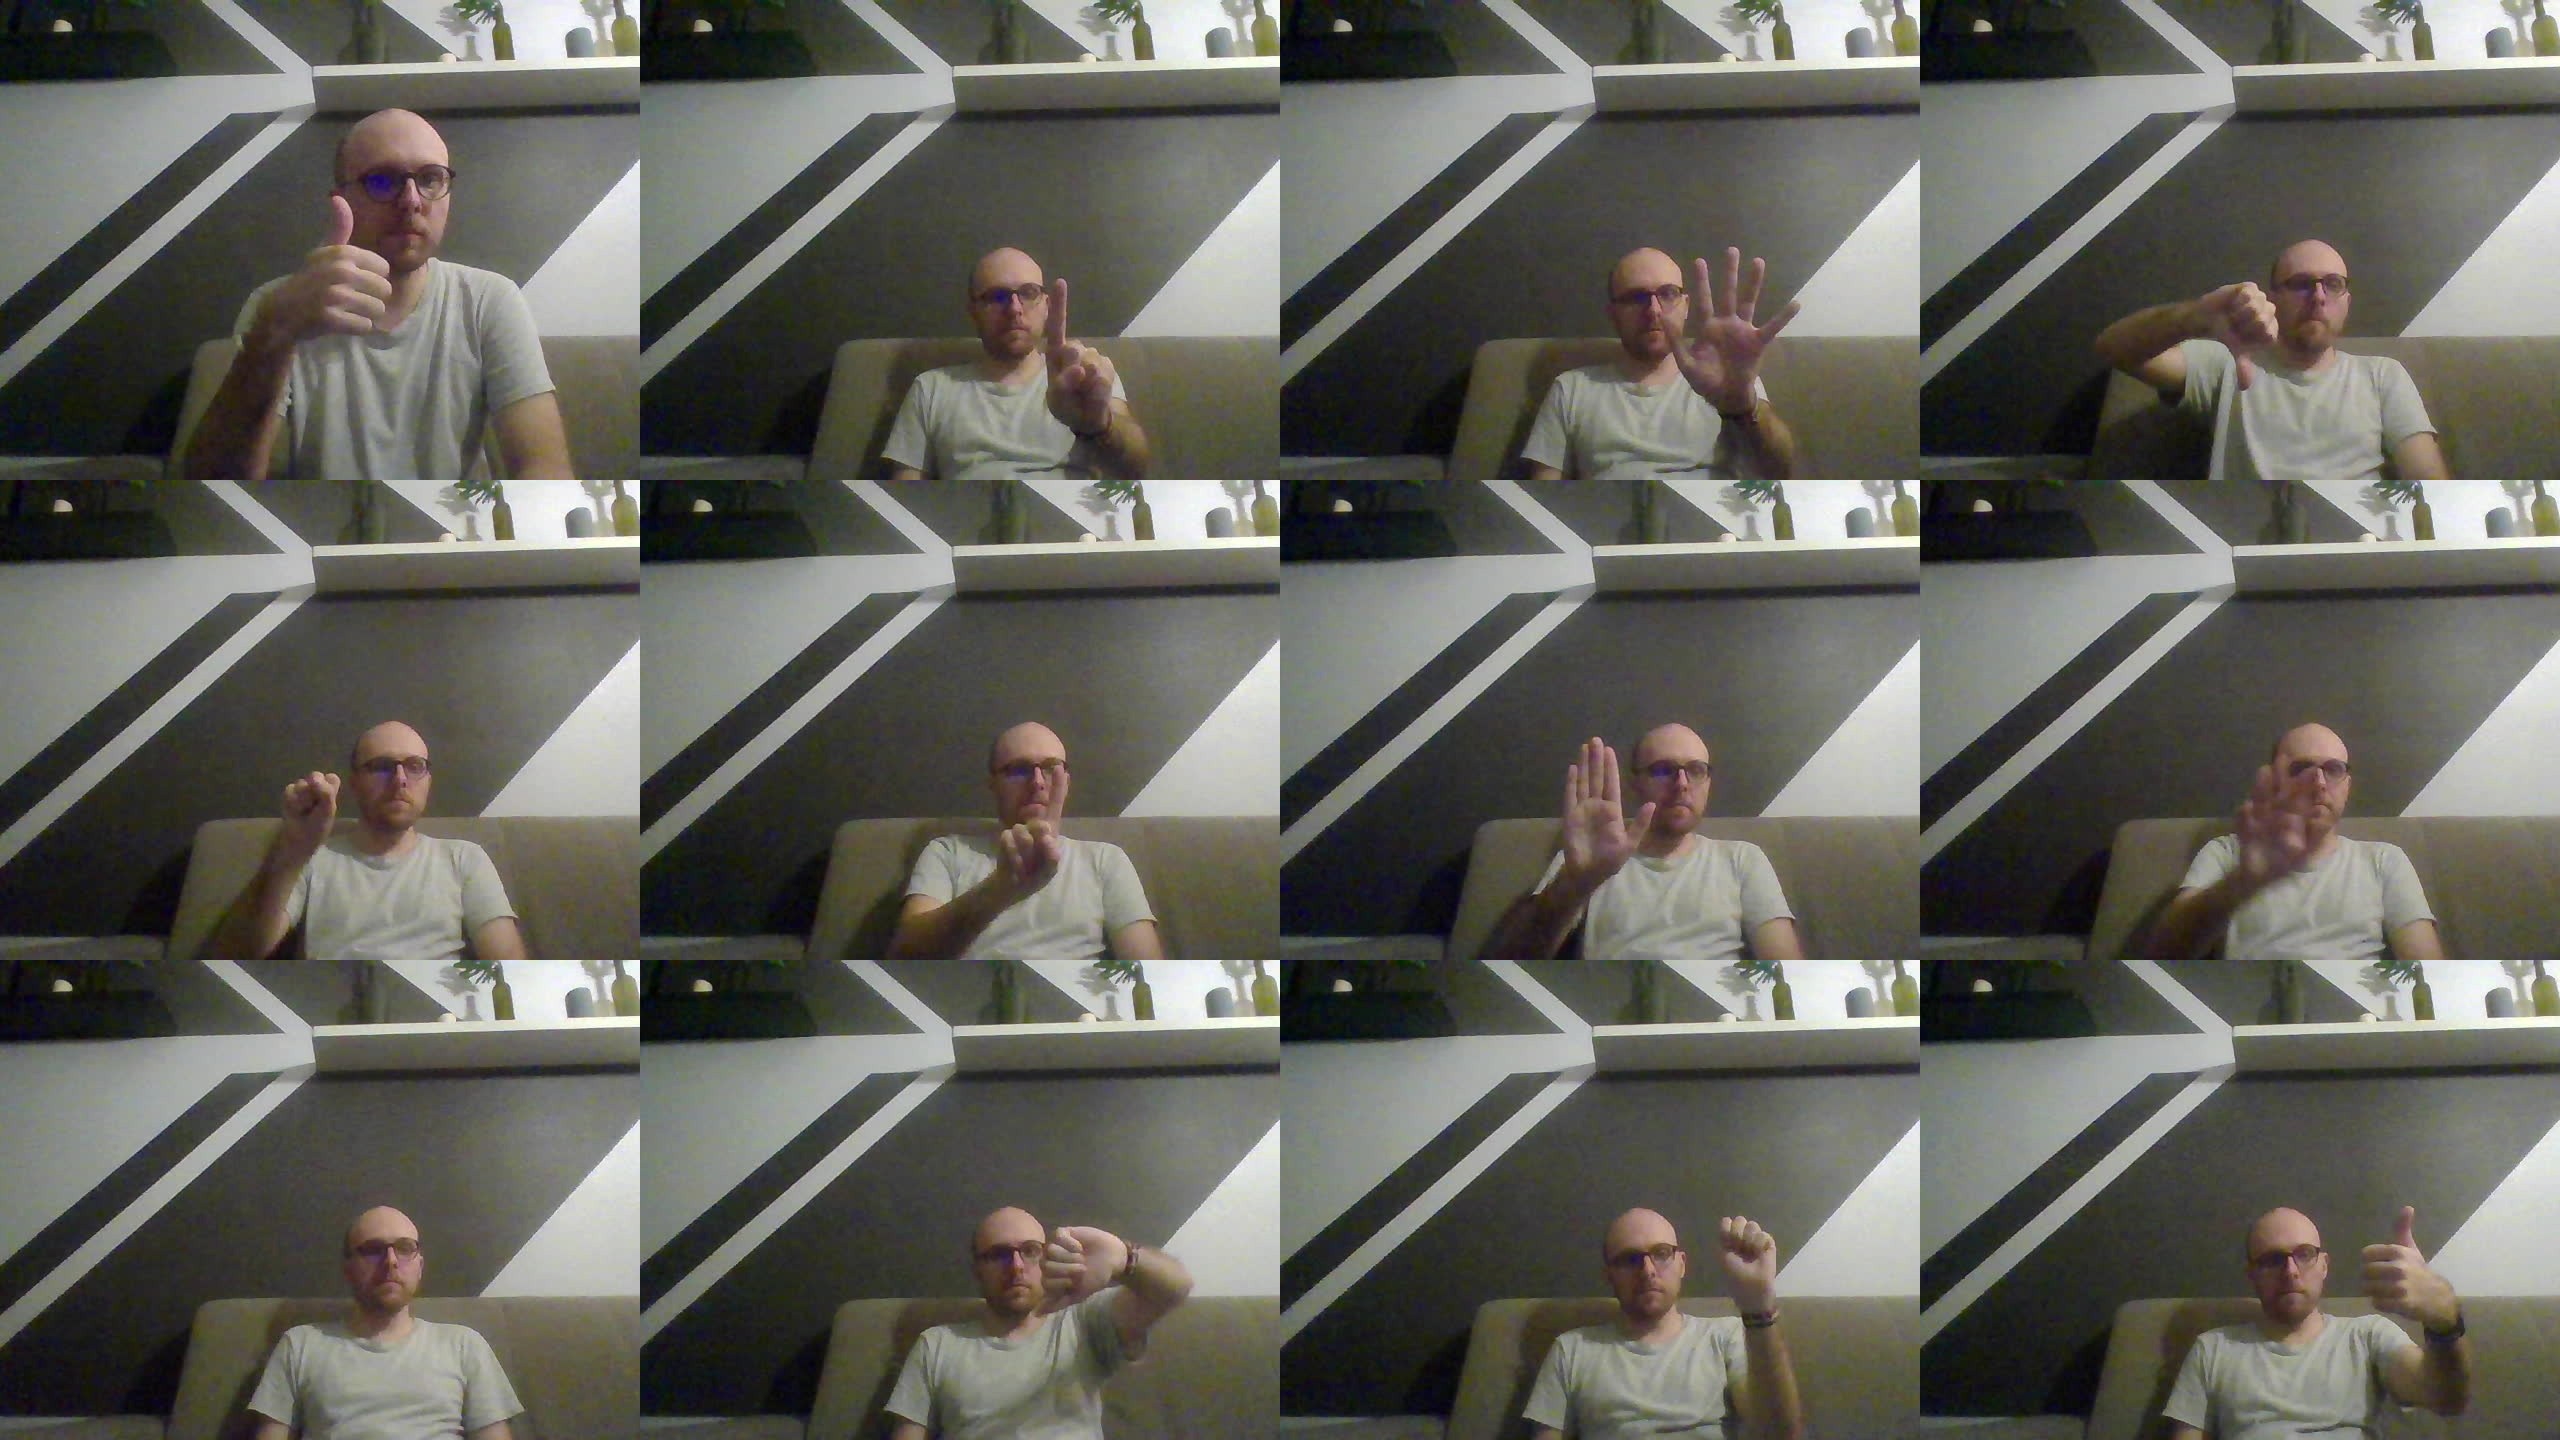
\includegraphics[width=\textwidth]{./pictures/pred_test.jpg}
  \caption{A simple dataset of 12 pictures showing a user doing different hand gestures. Poor quality footage, with a decent amount of noise, less-than-optimal luminosity and vague hand gestures were used in order to challange the models.}
  \label{fig:predtest}
\end{figure}

\begin{figure}[H]
  \centering
  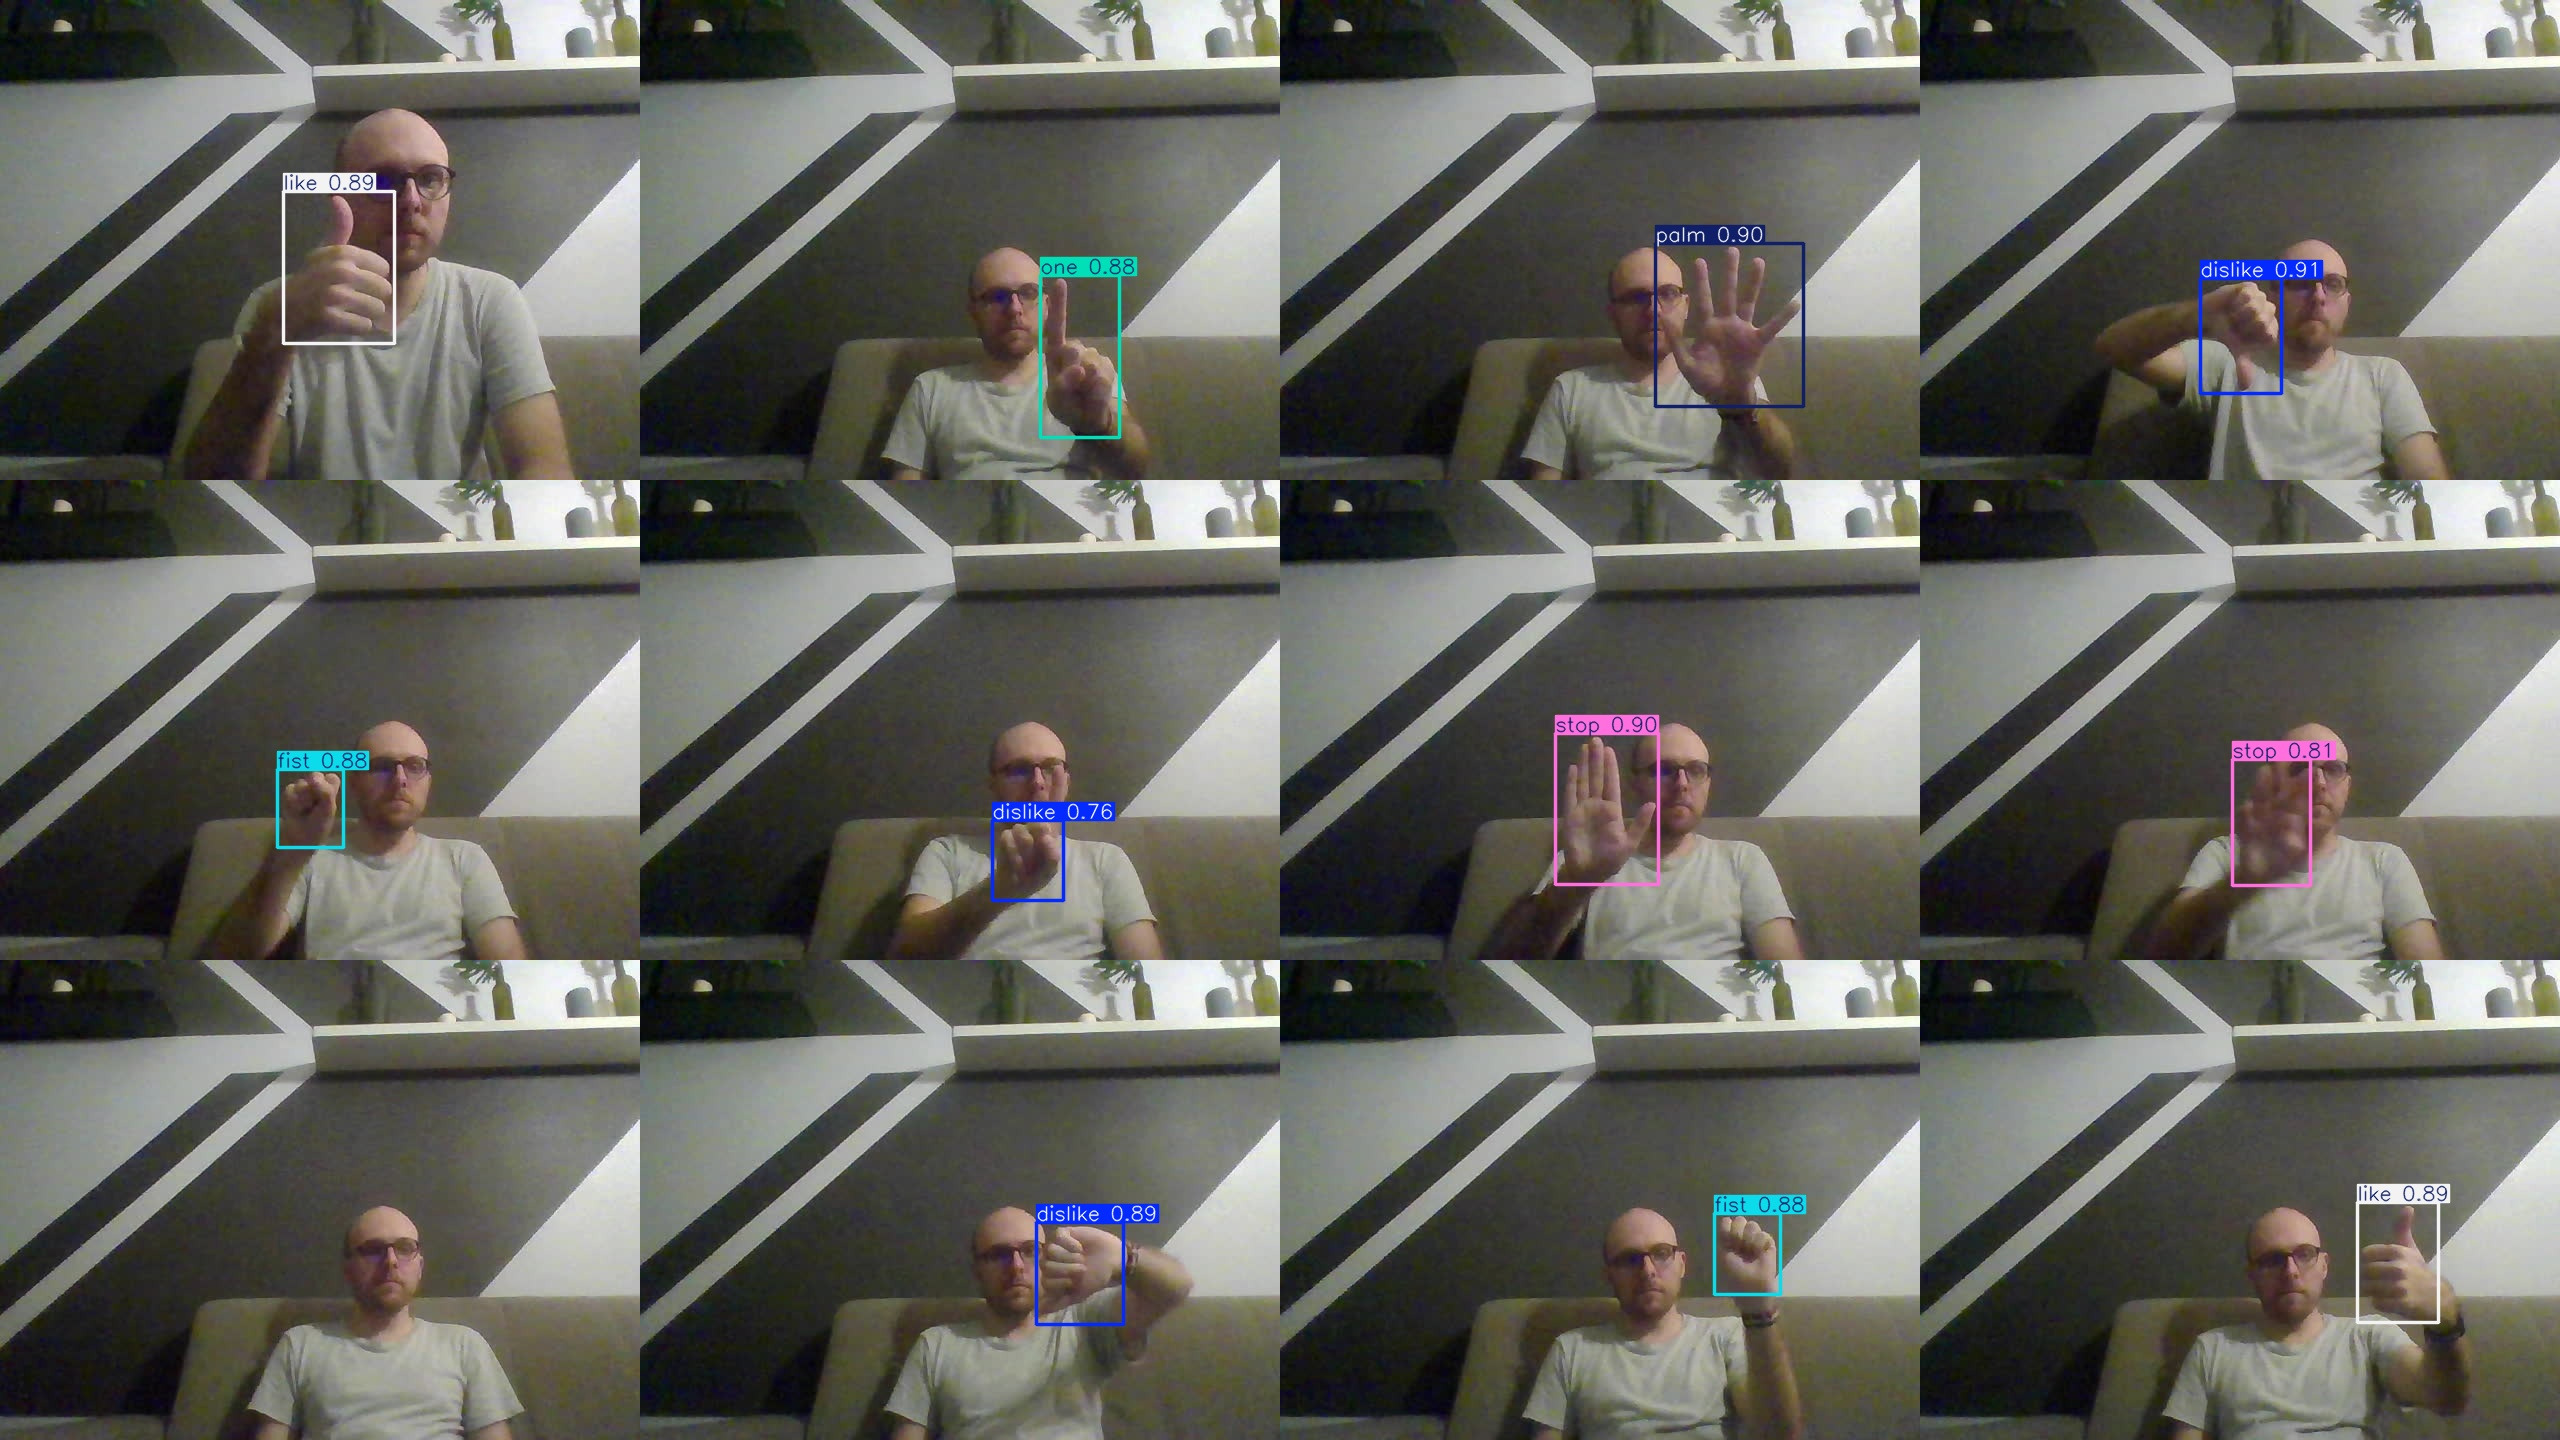
\includegraphics[width=\textwidth]{./pictures/smallhands_dell.jpg}
  \caption{ Predictions using the object detection model on the Dell Latitude laptop.}
  \label{fig:objdell}
\end{figure}

\begin{figure}[H]
  \centering
  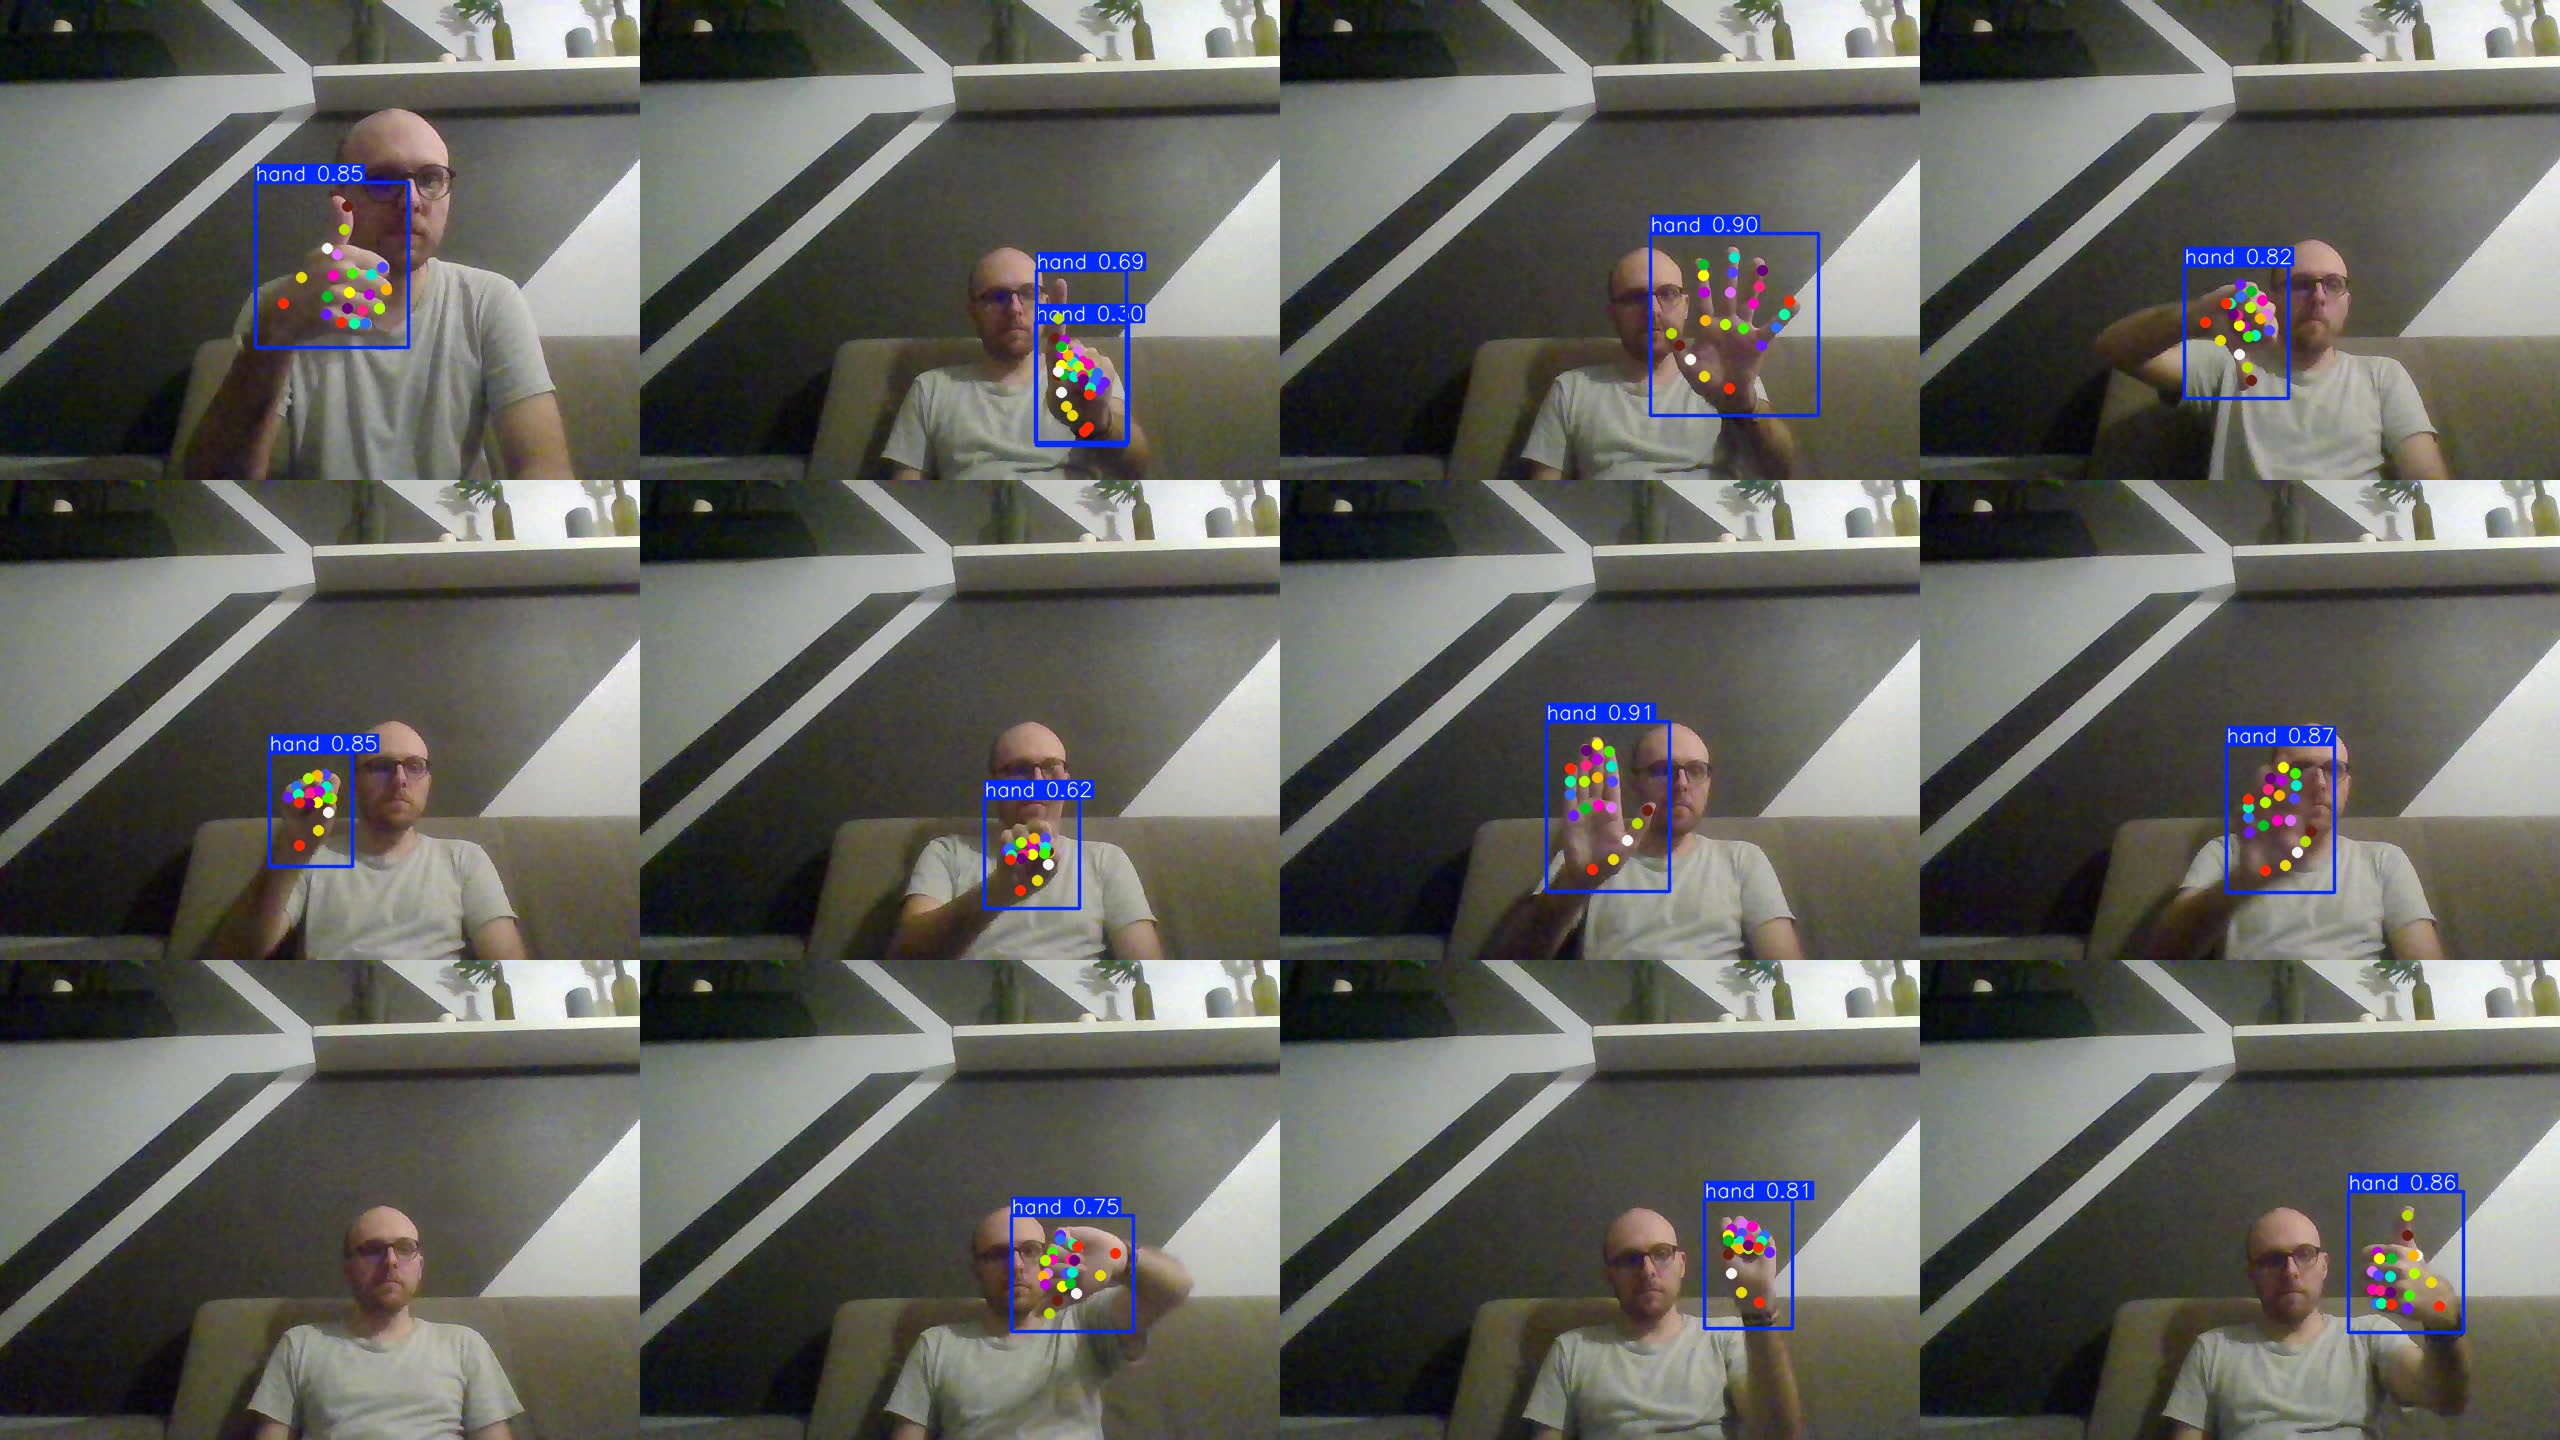
\includegraphics[width=\textwidth]{./pictures/pose_dell.jpg}
  \caption{Predictions using the pose estimation model on the Dell Latitude laptop.}
  \label{fig:posedell}
\end{figure}

\begin{figure}[H]
  \centering
  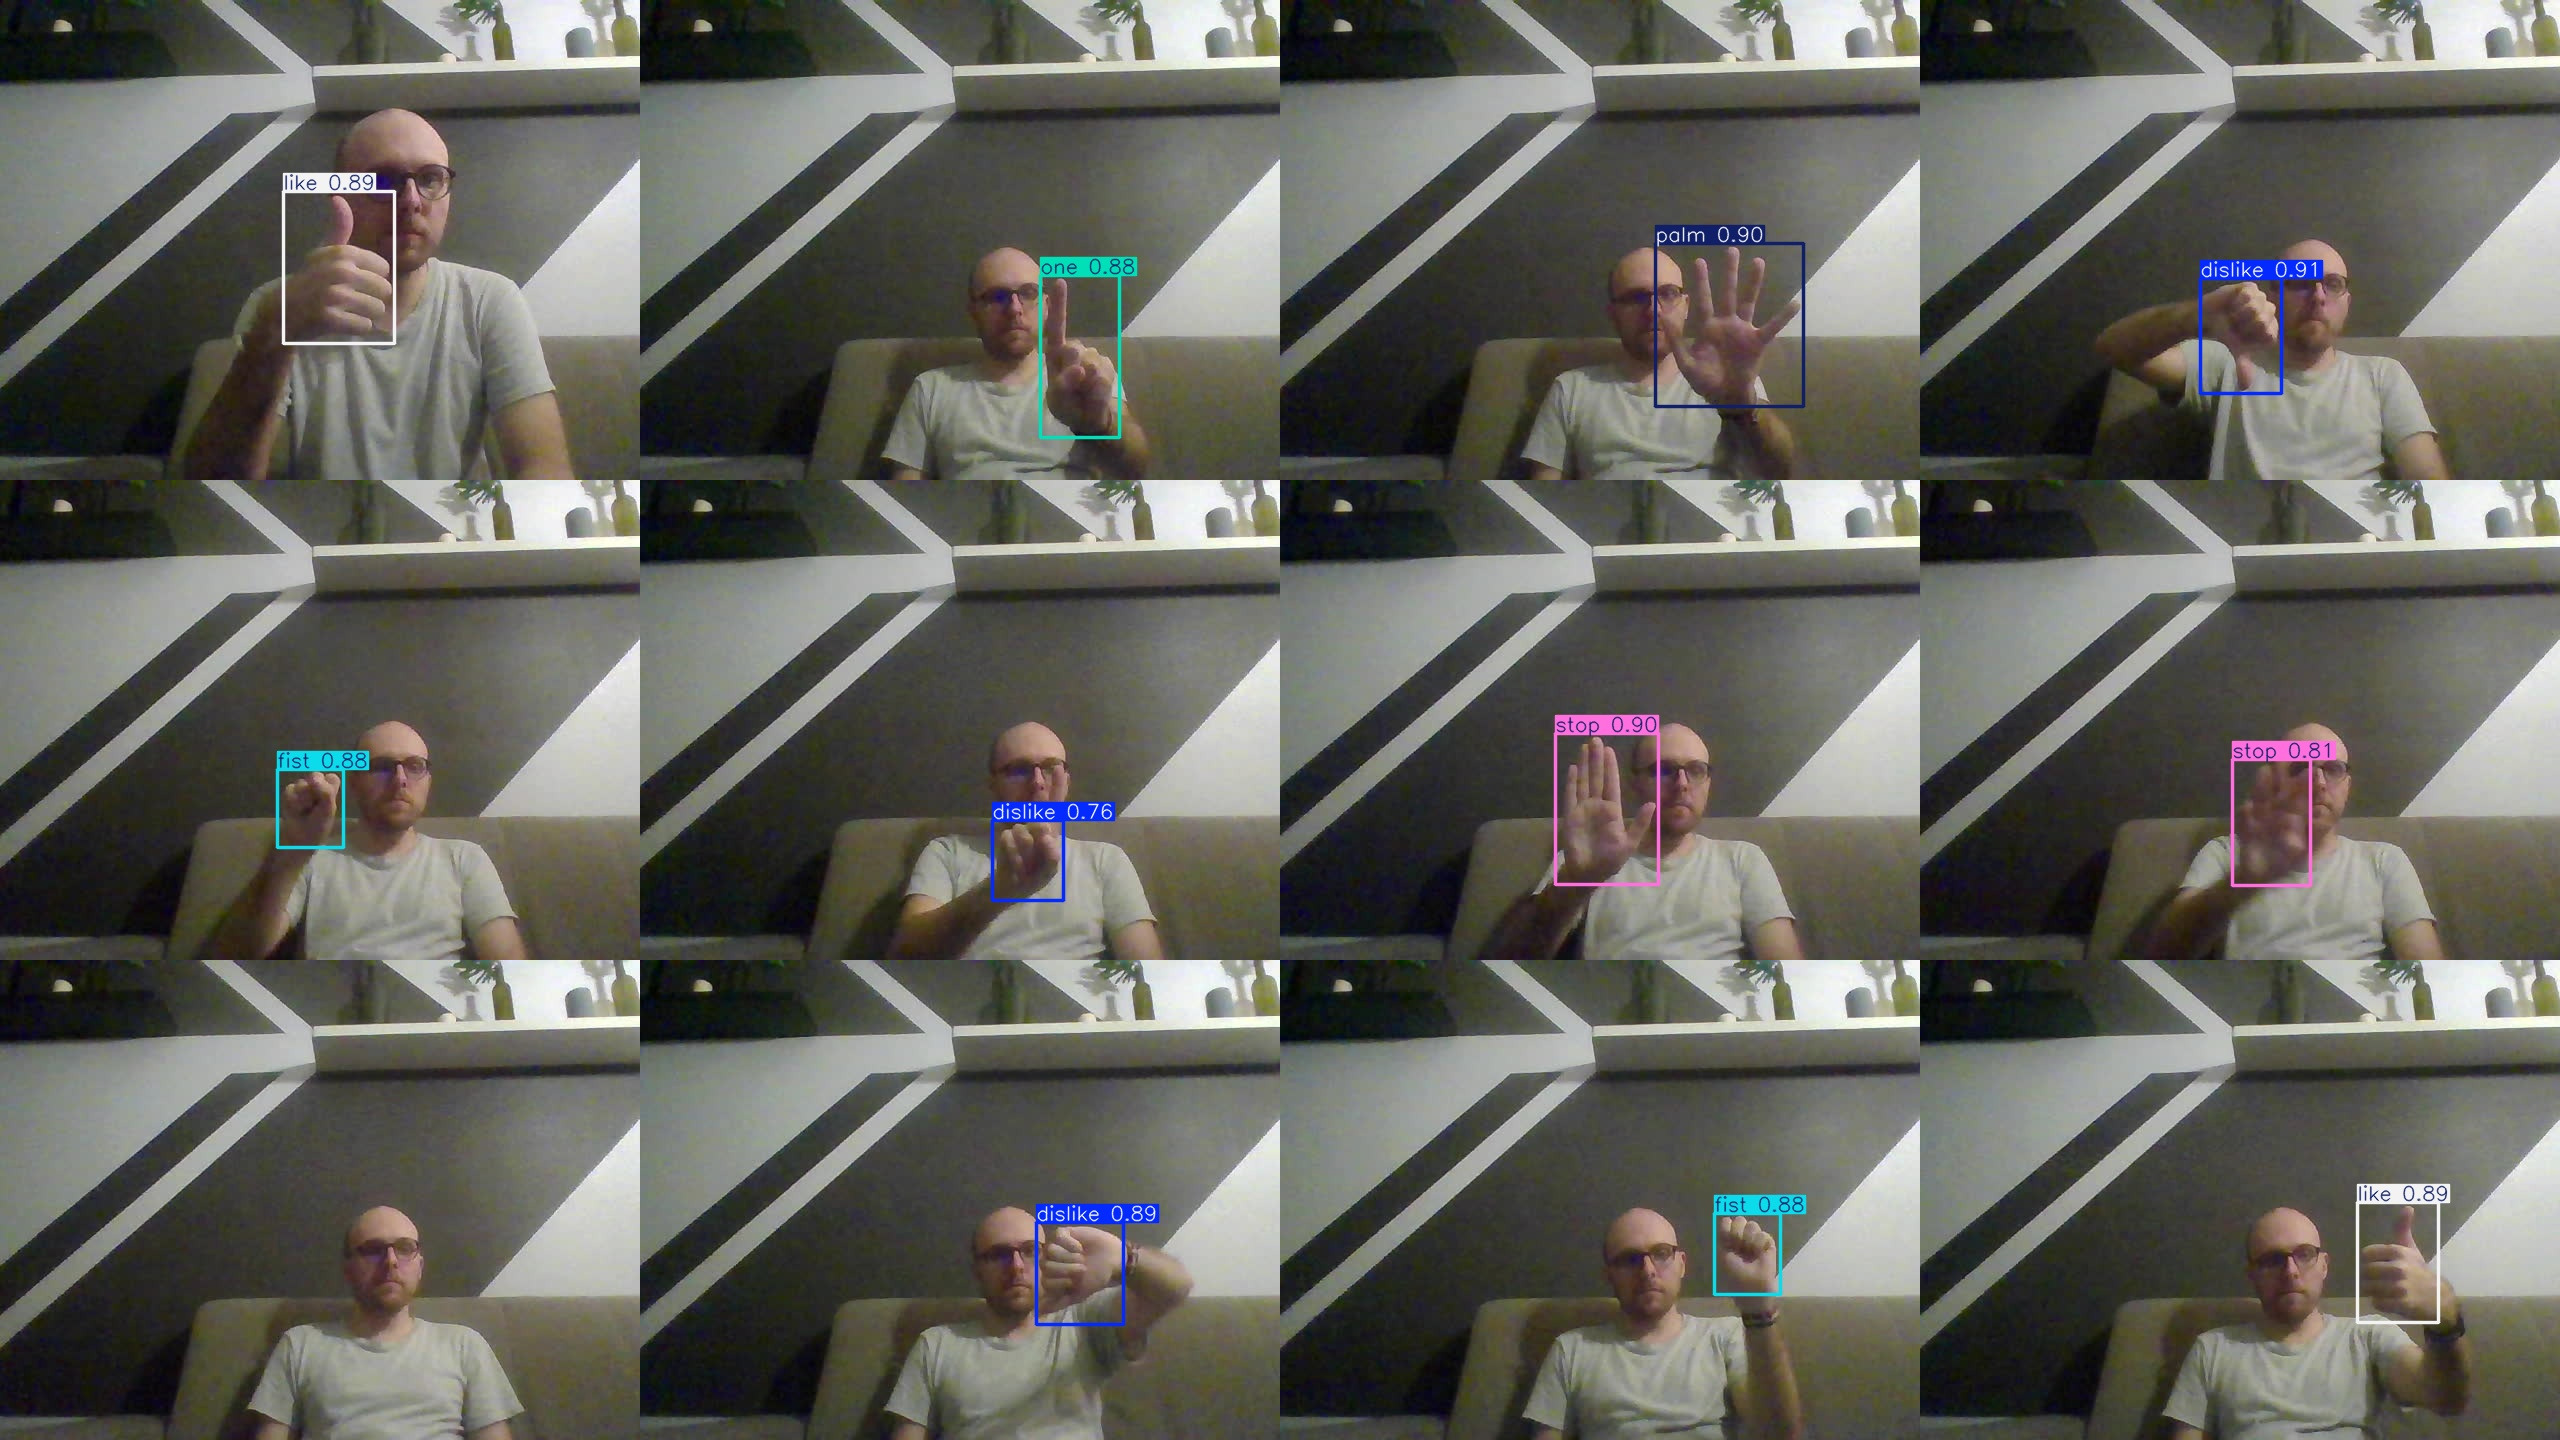
\includegraphics[width=\textwidth]{./pictures/smallhands_rpi.jpg}
  \caption{Predictions using the object detection model on the Raspberry PI.}
  \label{fig:objrpi}
\end{figure}

\begin{figure}[H]
  \centering
  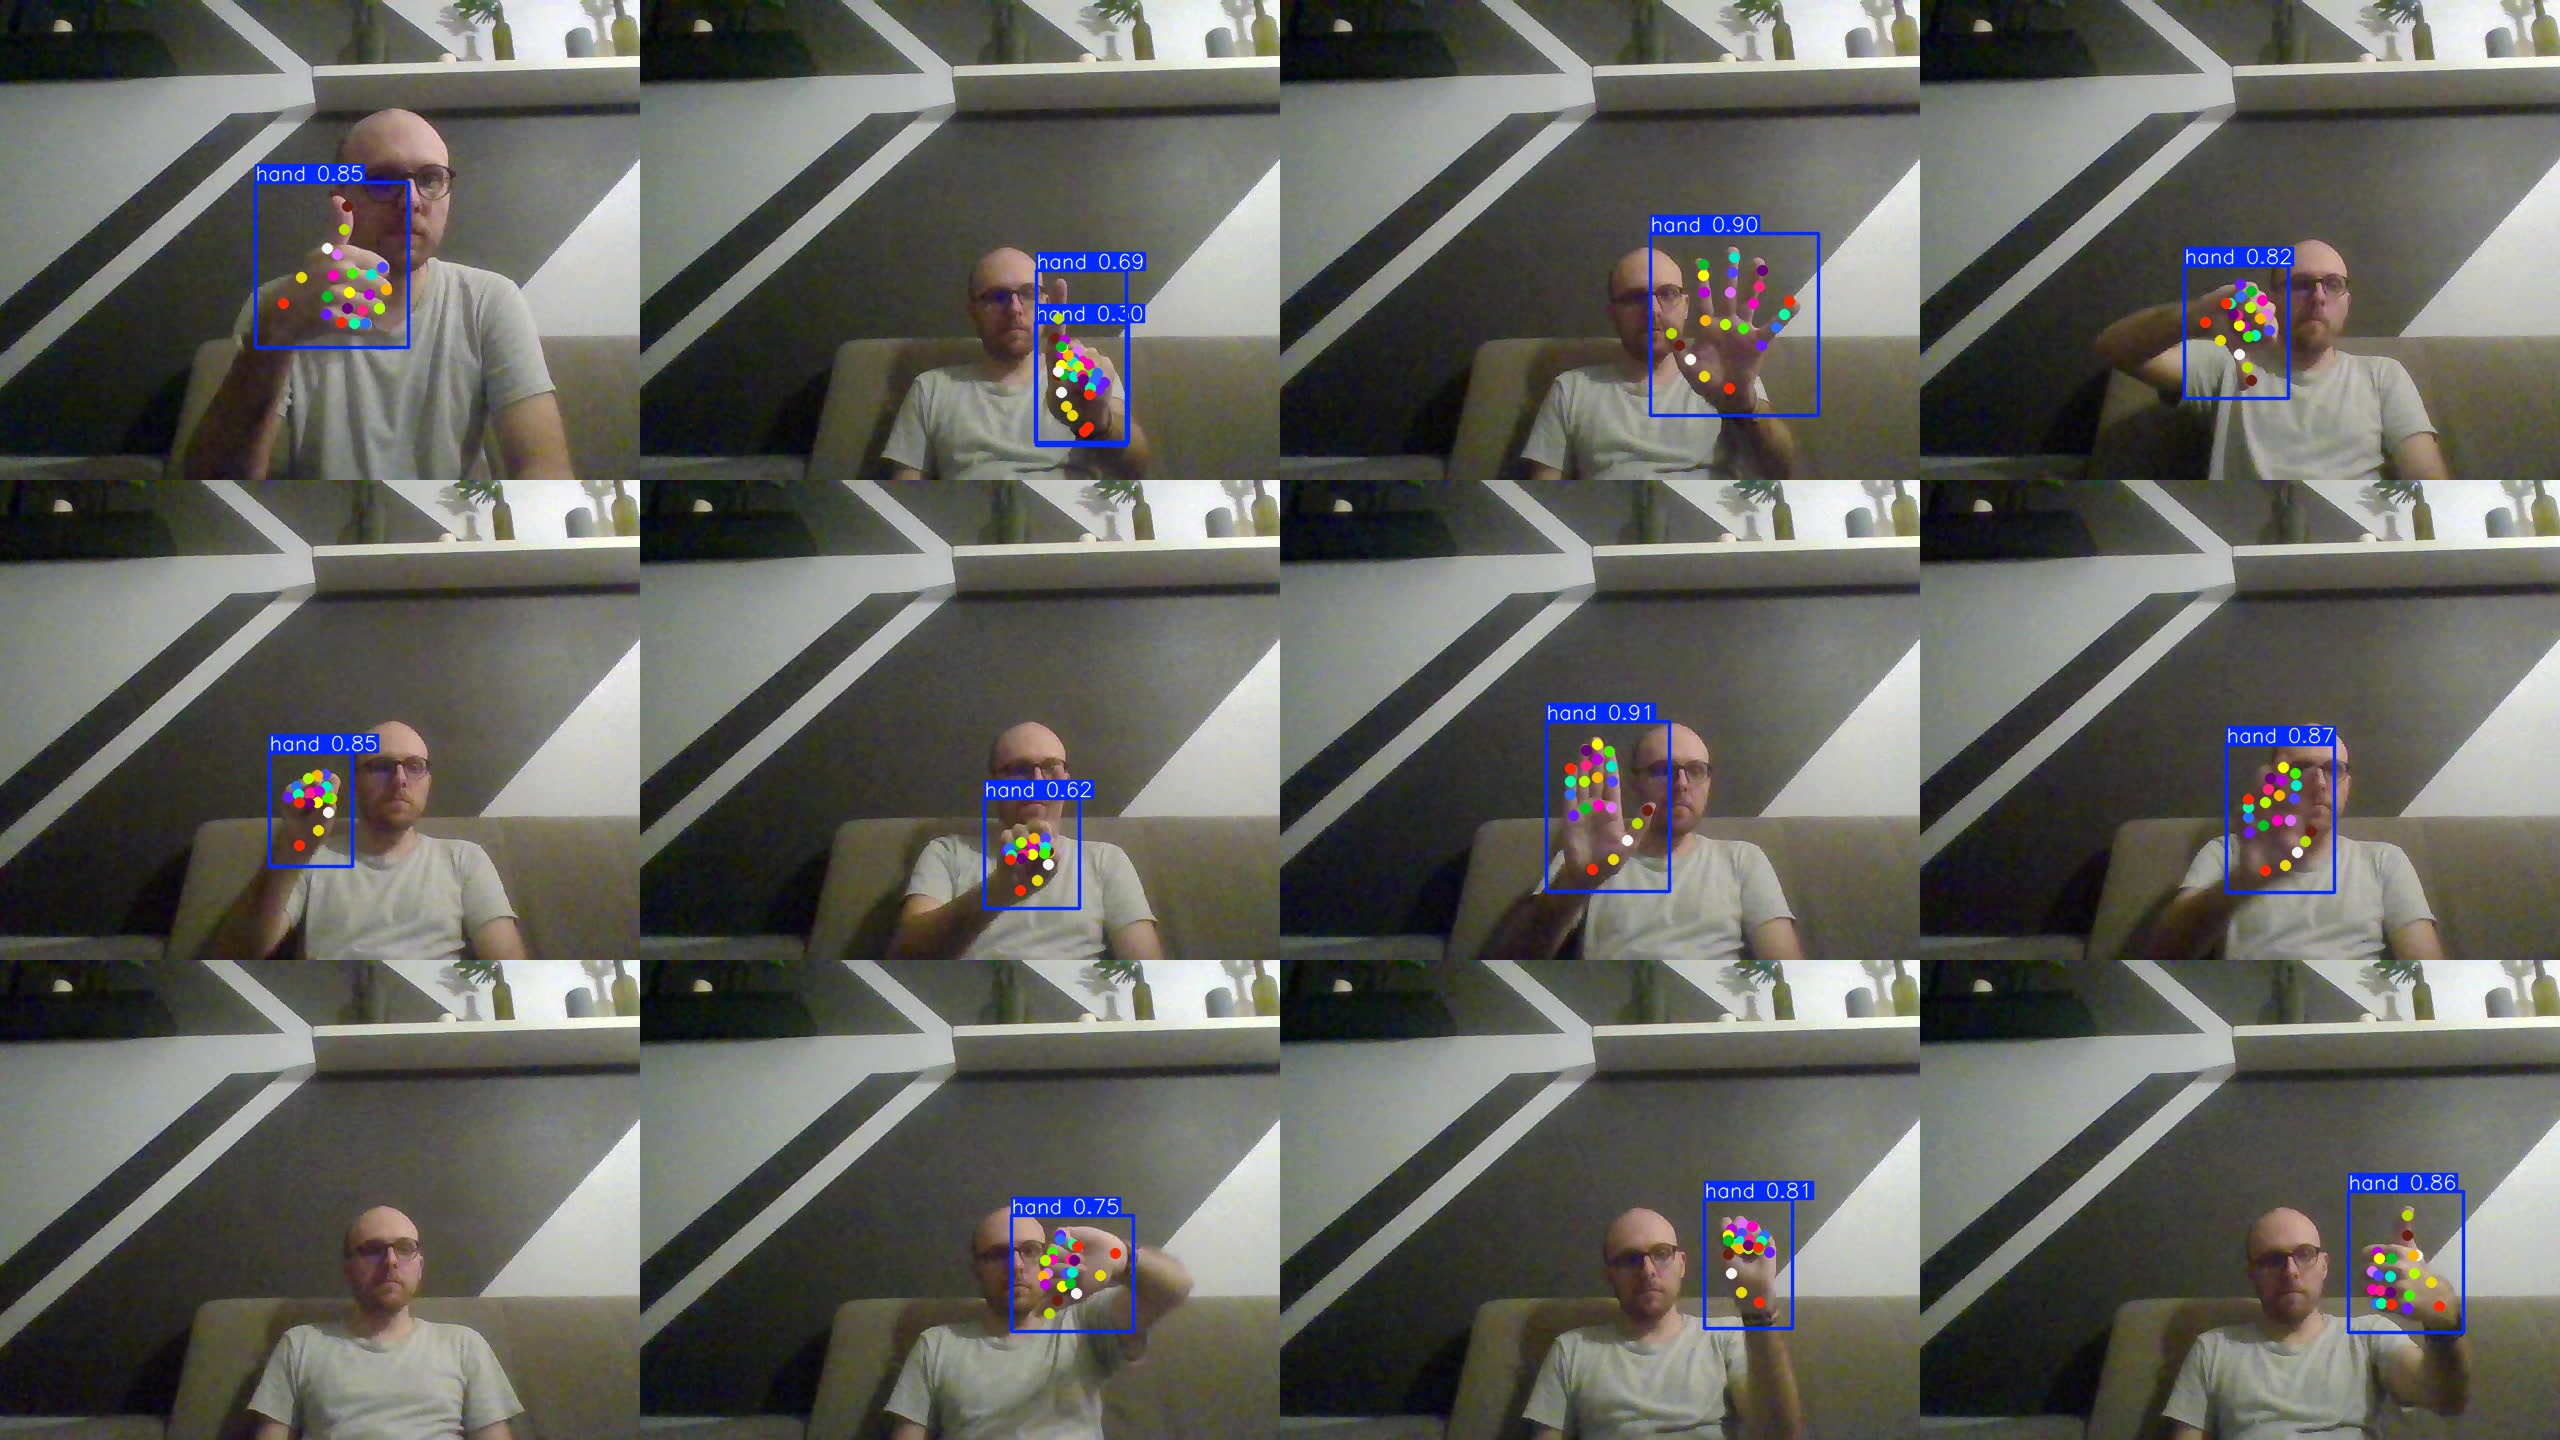
\includegraphics[width=\textwidth]{./pictures/pose_rpi.jpg}
  \caption{Predictions using the pose estimation model on the Raspberry PI.}
  \label{fig:poserpi}
\end{figure}

\section{References}
\bibliography{references}
\bibliographystyle{plain}

\end{document}

